% Document Preamble
\documentclass[aspectratio=169]{beamer}
\usetheme{metropolis}
\usepackage{blowup}
\blowUp{target=x3} % Makes the PDF a reasonable size frfr
\usepackage{hyperref}

\title{GE Silicone Sealants $^{222}$Rn Emanation Measurement}
\author[H. R. Glayzer]{H. Ryott Glayzer}
\institute[SDSMT]
{Lab Assistant\\
    SD Mines}
\date[2024]{February 2024}
\logo{
\includegraphics[height=1cm]{assets/SD_Mines_Logo.png}}

\begin{document}

\frame{\titlepage}

\begin{frame}{Overview of Emanation}
    Two samples were emanated throughout the latter half of 2023
    \begin{itemize}
        \item GE All-Purpose Silicone Sealant was emanated four times\\
            with a total of 465 hours of usable assay data.
        \item GE Advanced Silicone Sealant was emanated three times\\
            with a total of 895 hours of usable assay data.
    \end{itemize}
\end{frame}

\begin{frame}{Overview of GE All-Purpose Silicone Sealant Emanation}
    A sample of GE All-Purpose Silicone Sealant was emanated six times throughout Summer 2023.
        \begin{itemize}
            \item However, only four of those runs contained useful assay data,\@
                resulting in 465 hours of data available to analyze.
            \item The sample emanated had a surface area of approximately 200 cm$^{2}$
            \item Overall, the sample was determined to emanate at a rate of 0.00$^{+0.02}_{-0.00}$ mBq
            \begin{itemize}
                \item The uncertainties in this figure were calculated separately for top\@
                    and bottom errors in order to provide a more conservative estimate.
            \end{itemize}
        \end{itemize}
    This sample has an emanation rate sufficiently low for use in SuperCDMS
\end{frame}

\begin{frame}{GE All-Purpose Silicone Sealant}
    \begin{figure}
         \centering
        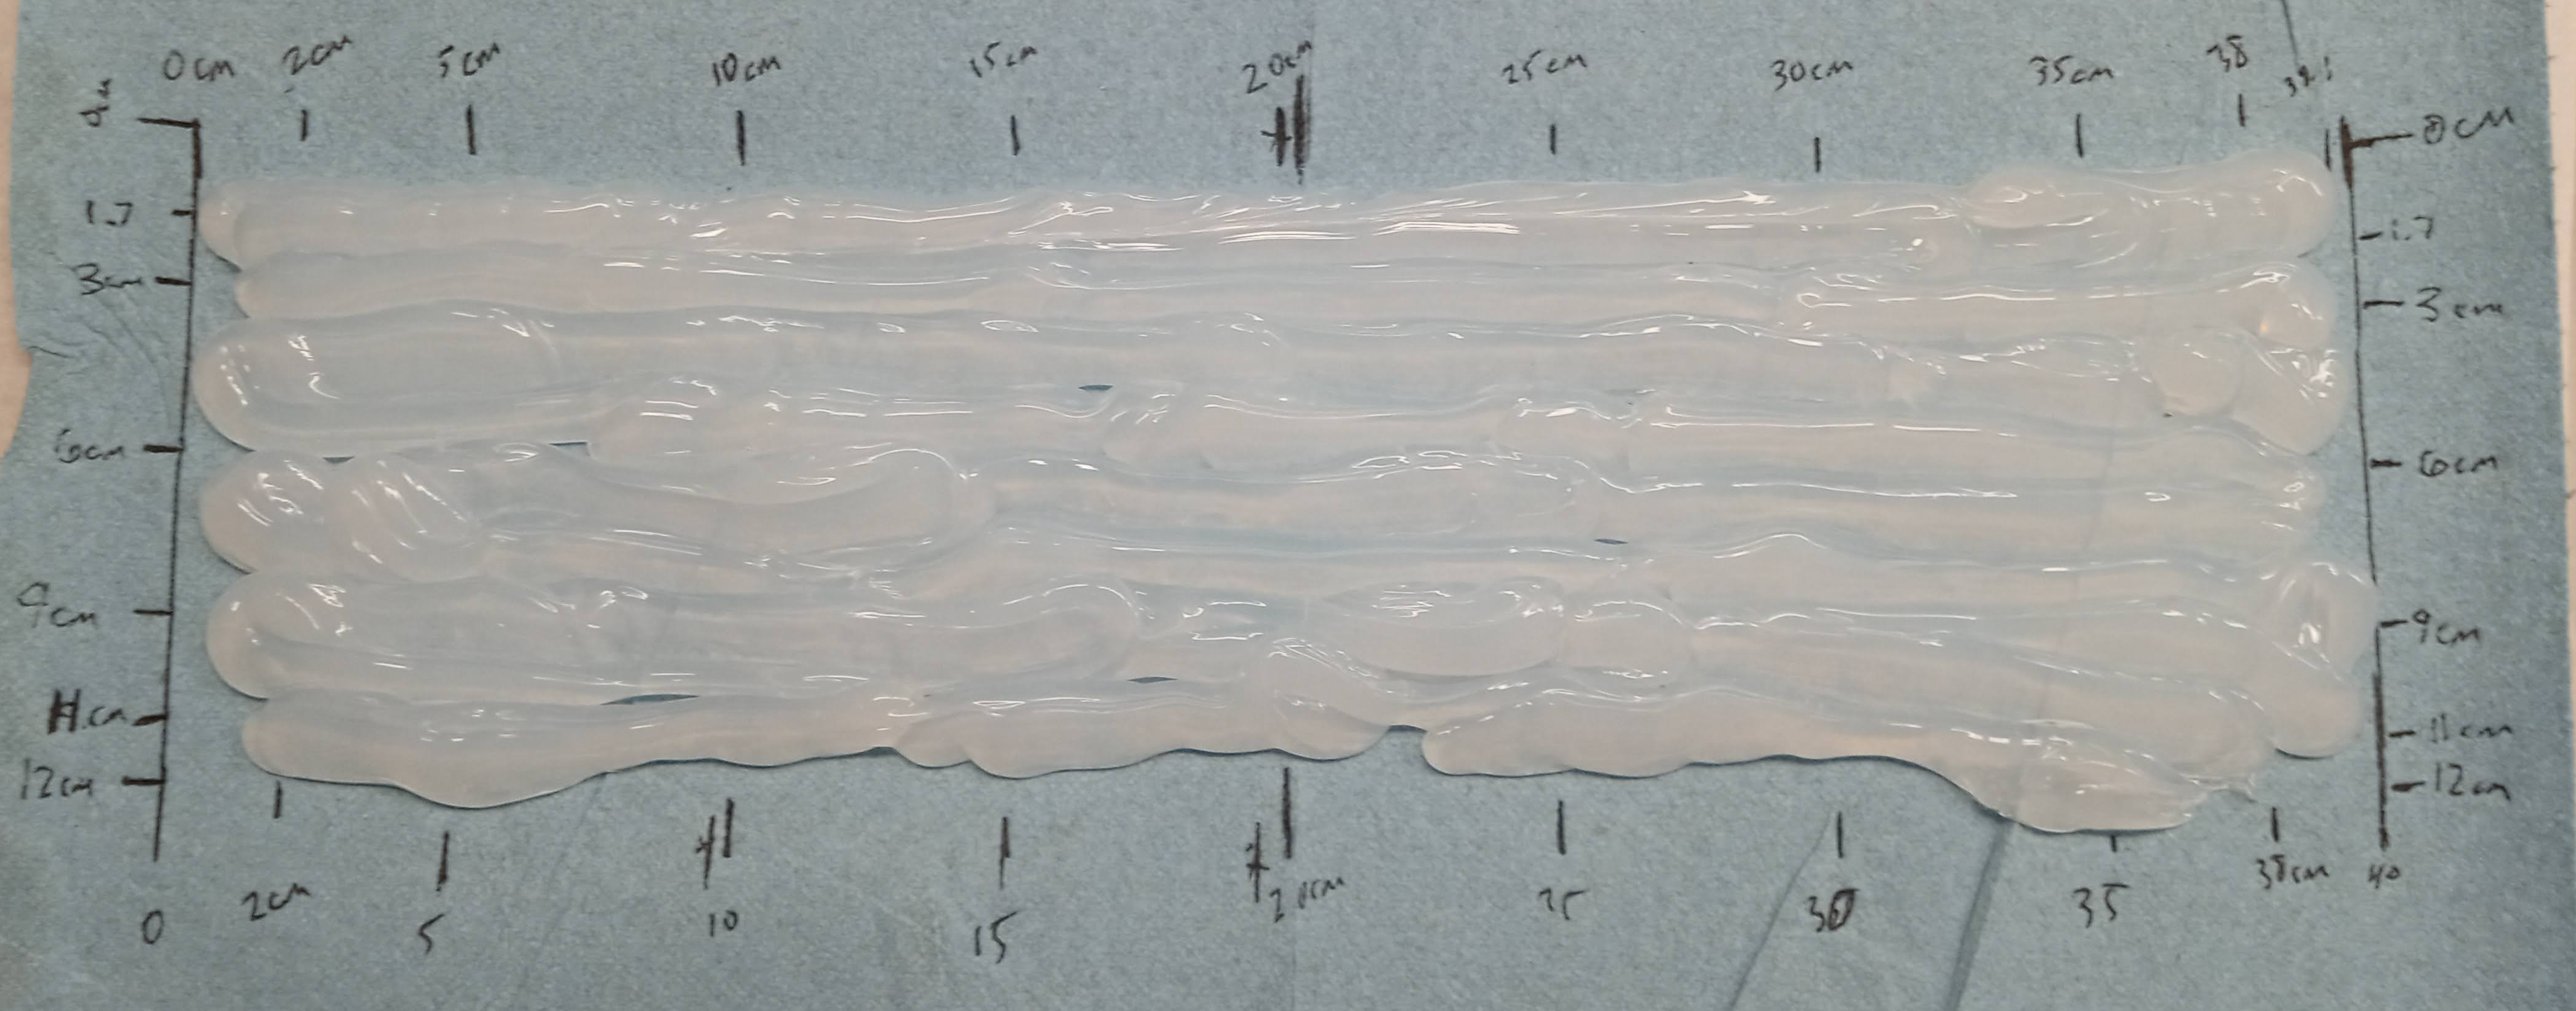
\includegraphics[width=0.85\textwidth]{assets/all-purpose-sample.png}
        \caption{GE All-Purpose Silicone Sealant}
    \end{figure}
\end{frame}

\begin{frame}{Run 717 Analysis}
    Run 717 occurred in June 2023.
    \begin{itemize}
        \item Emanation Rate was determined to be 0.00 $^{+0.03}_{-0.00}$ mBq.
        \item This determination was based on the observed emanation rate of $^{214}$Po.
        \item The $^{218}$Po rate wasn't used as poor resolution between the peaks of \@
            $^{218}$Po and $^{210}$Po likely caused $^{210}$Po events to spill over\@
            into the $^{218}$Po ROI
    \end{itemize}
    The Rate vs. Time plot for Run 717 follows.
   
    \hyperlink{717_Backup}{\beamerbutton{See backup slides for Run 717}}
\end{frame}

\begin{frame}{Rate vs. Time, Run 717}
\label{RvT_717}
    \begin{figure}
        \begin{center}
            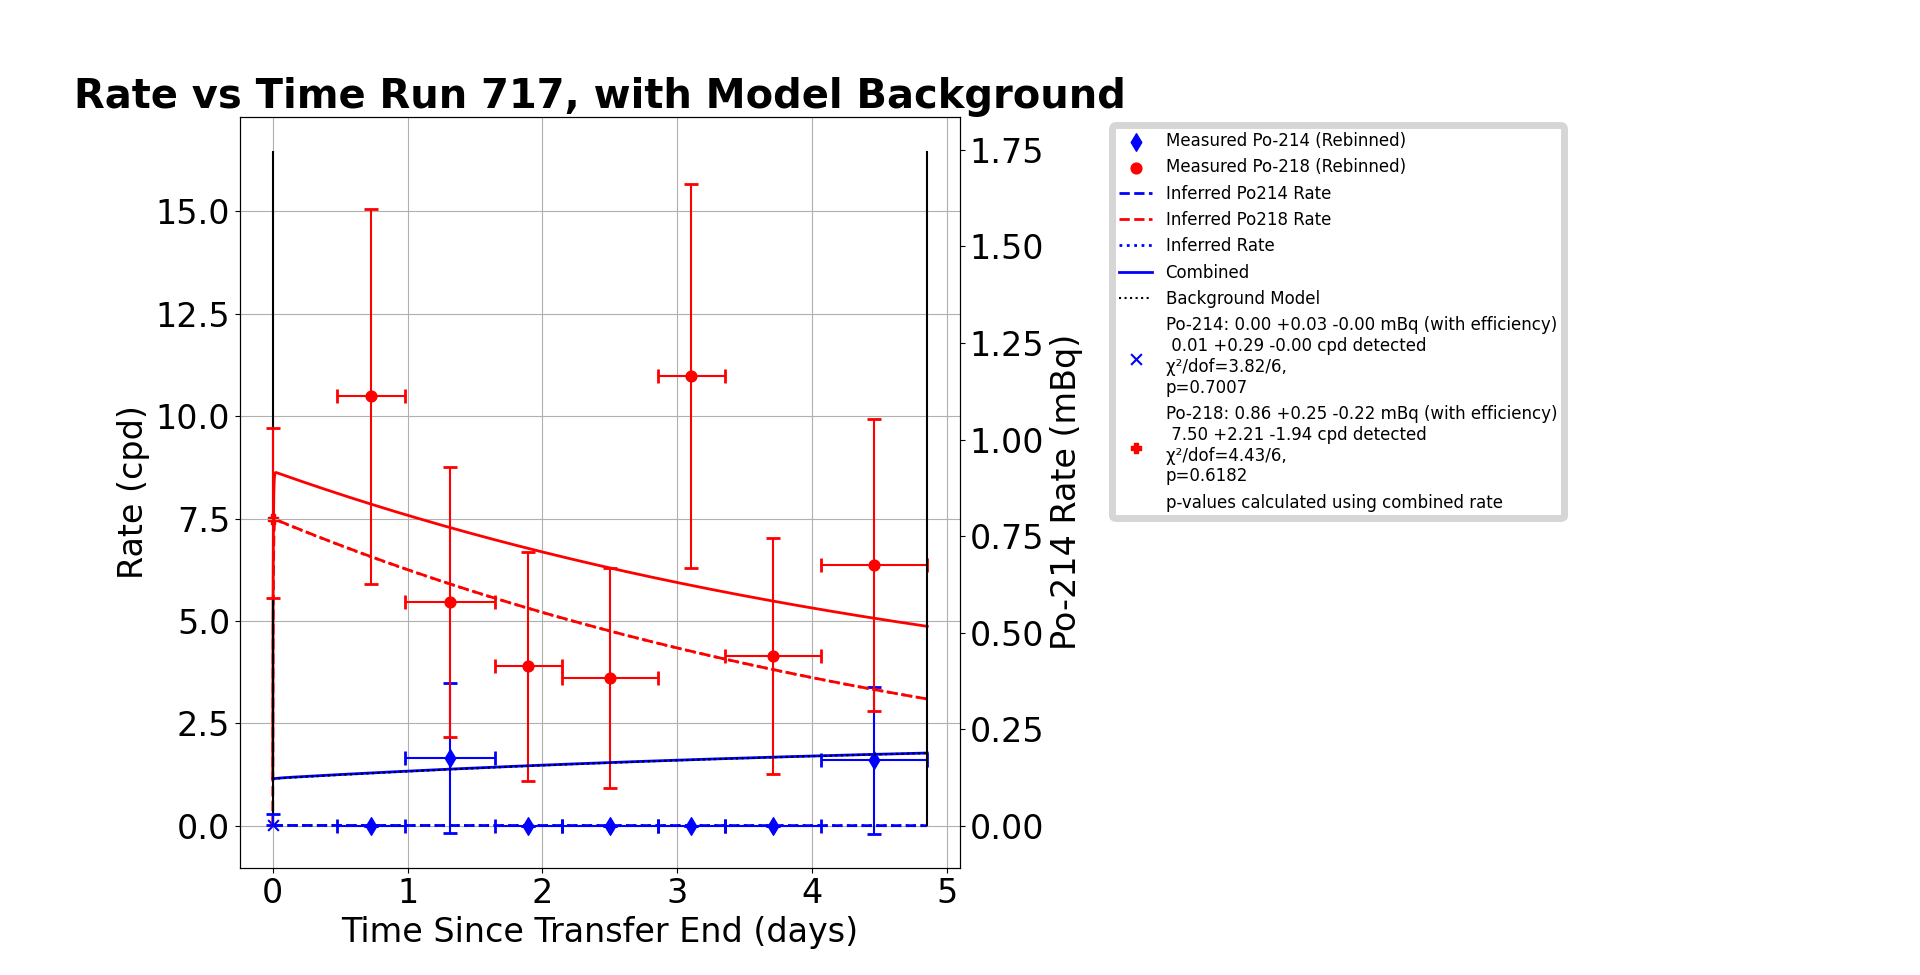
\includegraphics[width=0.9\textwidth]
            {assets/717/RvT.png}
            \caption{$^{222}$Rn Emanation Rate: 
            \textbf{0.00$^{+0.03}_{-0.00}$ mBq} (from $^{214}$Po Rate)}
        \end{center}
    \end{figure}  
\end{frame}

\begin{frame}{Run 720 Analysis}
    Run 720 occurred in June and July 2023.
    \begin{itemize}
        \item Emanation Rate was determined to be \textbf{0.00 $^{+0.54}_{-0.00}$ mBq}.
        \item This determination was based on the observed emanation rate of $^{214}$Po.
        \item The $^{218}$Po rate wasn't used as poor resolution between the peaks of \@
            $^{218}$Po and $^{210}$Po likely caused $^{210}$Po events to spill over\@
            into the $^{218}$Po ROI
    \end{itemize}

    \hyperlink{720_Backup}{\beamerbutton{See Backup Slides for Run 720}}
\end{frame}

\begin{frame}{Rate vs. Time, Run 720}
\label{RvT_720}
    \begin{figure}
        \begin{center}
            \includegraphics[width=0.9\textwidth]
            {assets/720/RvT.png}
            \caption{$^{222}$Rn Emanation Rate: 
            \textbf{0.00$^{+0.54}_{-0.00}$ mBq} (from $^{214}$Po rate)}
        \end{center}
    \end{figure}    
\end{frame}

\begin{frame}{Run 721 Analysis}
    \begin{itemize}
        \item Emanation Rate was determined to be \textbf{0.00 $^{+0.02}_{-0.00}$ mBq}.
        \item This determination was based on the observed emanation rate of $^{214}$Po.
        \item The $^{218}$Po rate wasn't used as poor resolution between the peaks of \@
            $^{218}$Po and $^{210}$Po likely caused $^{210}$Po events to spill over\@
            into the $^{218}$Po ROI
    \end{itemize}

    \hyperlink{721_Backup}{\beamerbutton{See Backup Slides for Run 721}}
\end{frame}

\begin{frame}{Rate vs. Time, Run 721}
\label{RvT_721}
    \begin{figure}
        \begin{center}
            \includegraphics[width=0.9\textwidth]
            {assets/721/RvT.png}
            \caption{$^{222}$Rn Emanation Rate: 
            \textbf{0.00$^{+0.02}_{-0.00}$ mBq} (from $^{214}$Po rate)}
        \end{center}
    \end{figure}    
\end{frame}

\begin{frame}{Run 722 Analysis}
    \begin{itemize}
        \item Emanation Rate was determined to be \textbf{0.177 $^{+0.096}_{-0.081}$ mBq}.
        \item This determination was based on the combined rates $^{214}$Po and $^{218}$Po.
    \end{itemize}

    \hyperlink{722_Backup}{\beamerbutton{See Backup Slides for Run 722}}
\end{frame}

\begin{frame}{Rate vs. Time, Run 722}
\label{RvT_722}
    \begin{figure}
        \begin{center}
            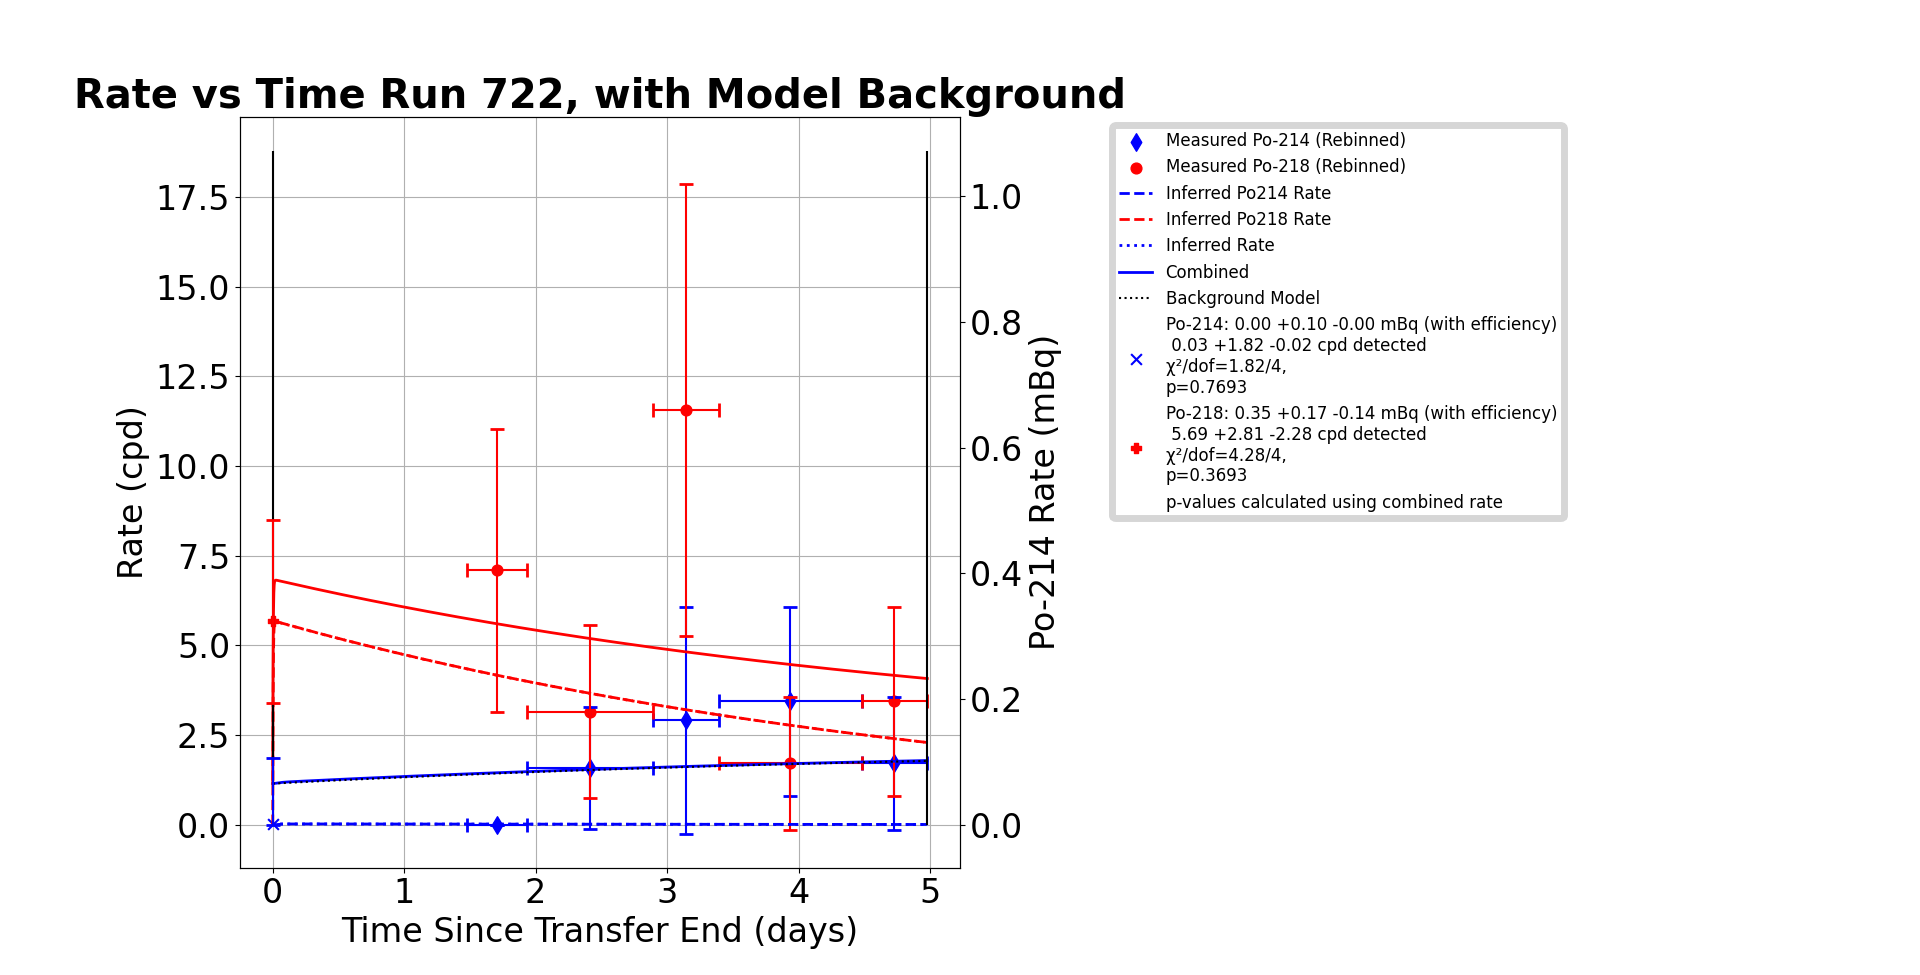
\includegraphics[width=0.9\textwidth]
            {assets/722/RvT.png}
            \caption{$^{222}$Rn Emanation Rate: 
            \textbf{0.177$^{+0.096}_{-0.081}$ mBq} (from combined rate)}
        \end{center}
    \end{figure}    
\end{frame}

\begin{frame}{Overview of GE Advanced Silicone Sealant Emanation}
    A sample of GE Advanced Silicone Sealant was emanated four times throughout late 2023.
    \begin{itemize}
        \item These rhns resulted in a total of 895 Hours of useful assay data
    \end{itemize}
    These runs resulted in a total of 895 Hours of useful assay data.
   
    Overall, the GE Advanced Silicone Sealant was measured

\end{frame}

\begin{frame}{Run 730 Analysis}
    \begin{itemize}
        \item Emanation Rate was determined to be \textbf{0.001 $^{+0.013}_{-0.000}$ mBq}.
        \item This determination was based on the combined rates $^{214}$Po and $^{218}$Po.
    \end{itemize}
    This run exhibited fair resolution between $^{21x}$Po event peaks.

    \hyperlink{730_Backup}{\beamerbutton{See Backup Slides for Run 730}}
\end{frame}

\begin{frame}{Rate vs. Time, Run 730}
\label{RvT_730}
    \begin{figure}
        \begin{center}
            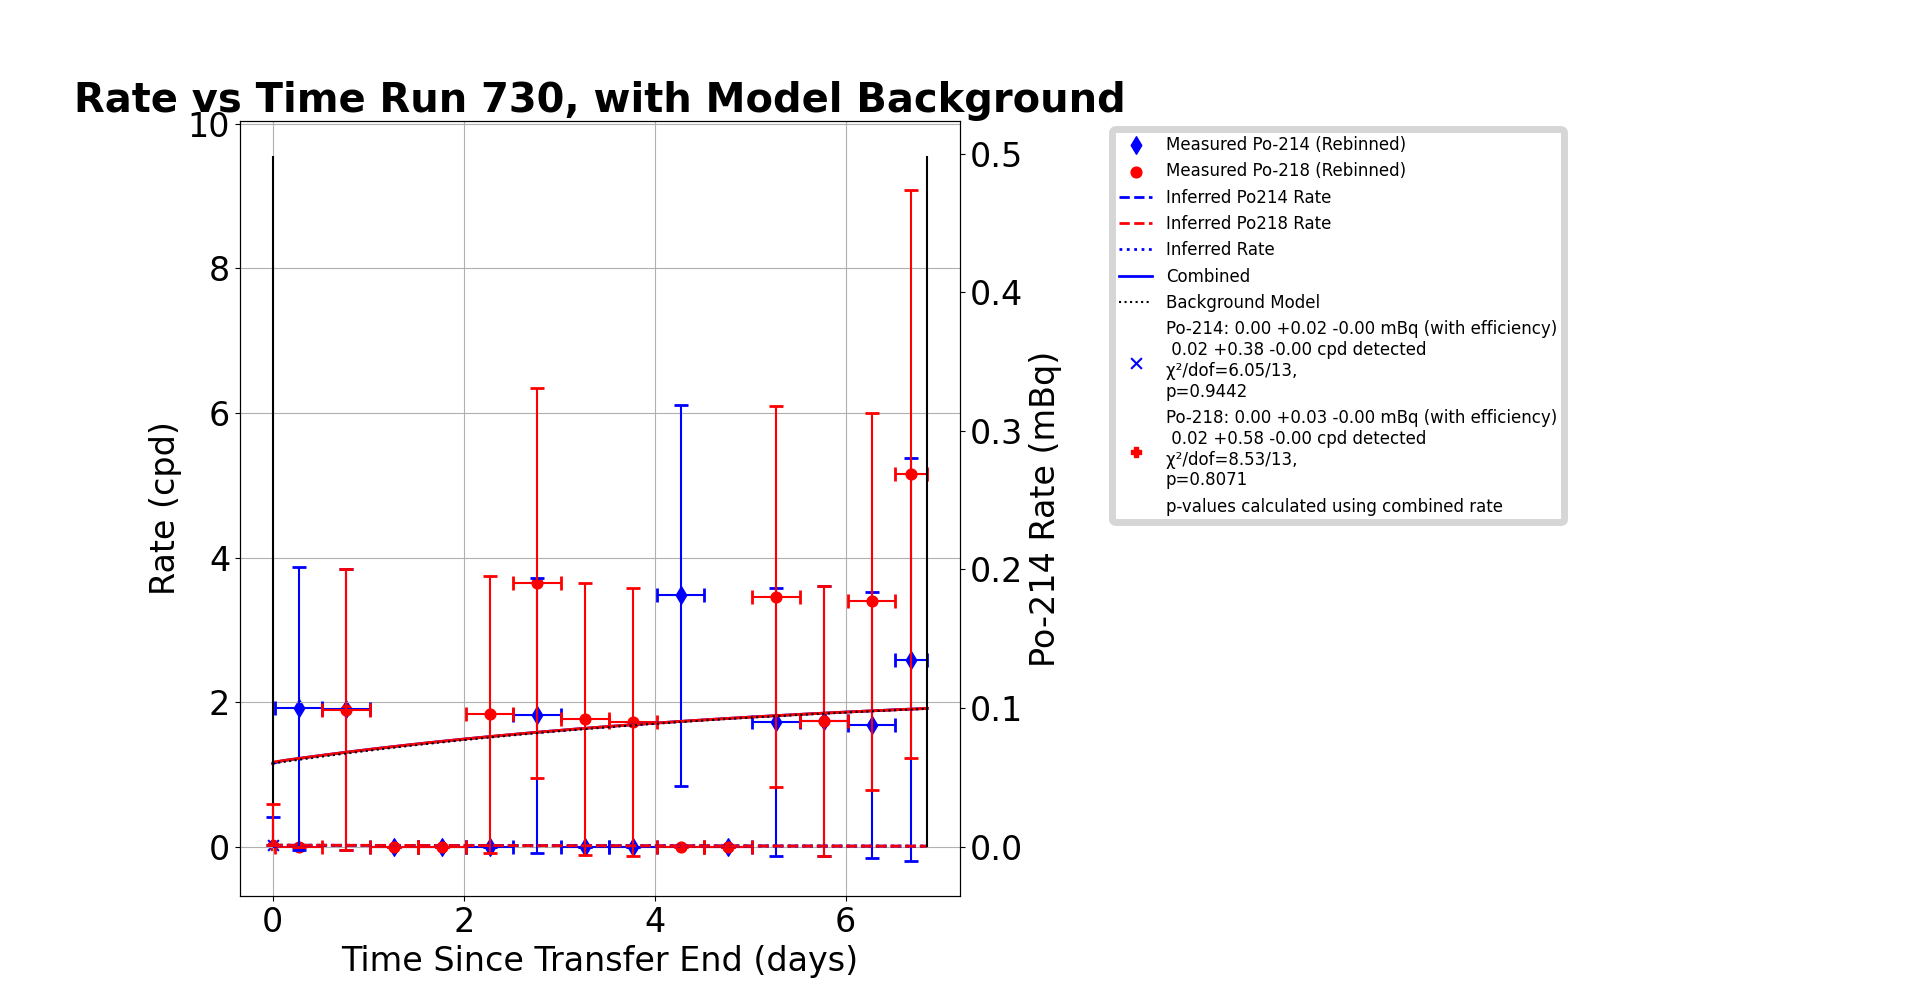
\includegraphics[width=0.9\textwidth]
            {assets/730/RvT.png}
            \caption{$^{222}$Rn Emanation Rate: 
            \textbf{0.001$^{+0.013}_{-0.000}$ mBq} (from combined rate)}
        \end{center}
    \end{figure}    
\end{frame}

\begin{frame}{Backup Slides}
    Backup Slides contain additional data and information that may be helpful
    to provide context if questions come up.
\end{frame}

\begin{frame}{Run 717 Backup Slides}
\label{717_Backup}
    The following slides contain additional data and information regarding Run 717.
\end{frame}

\begin{frame}{Raw Data, Run 717}
    \begin{figure}
        \begin{center}
            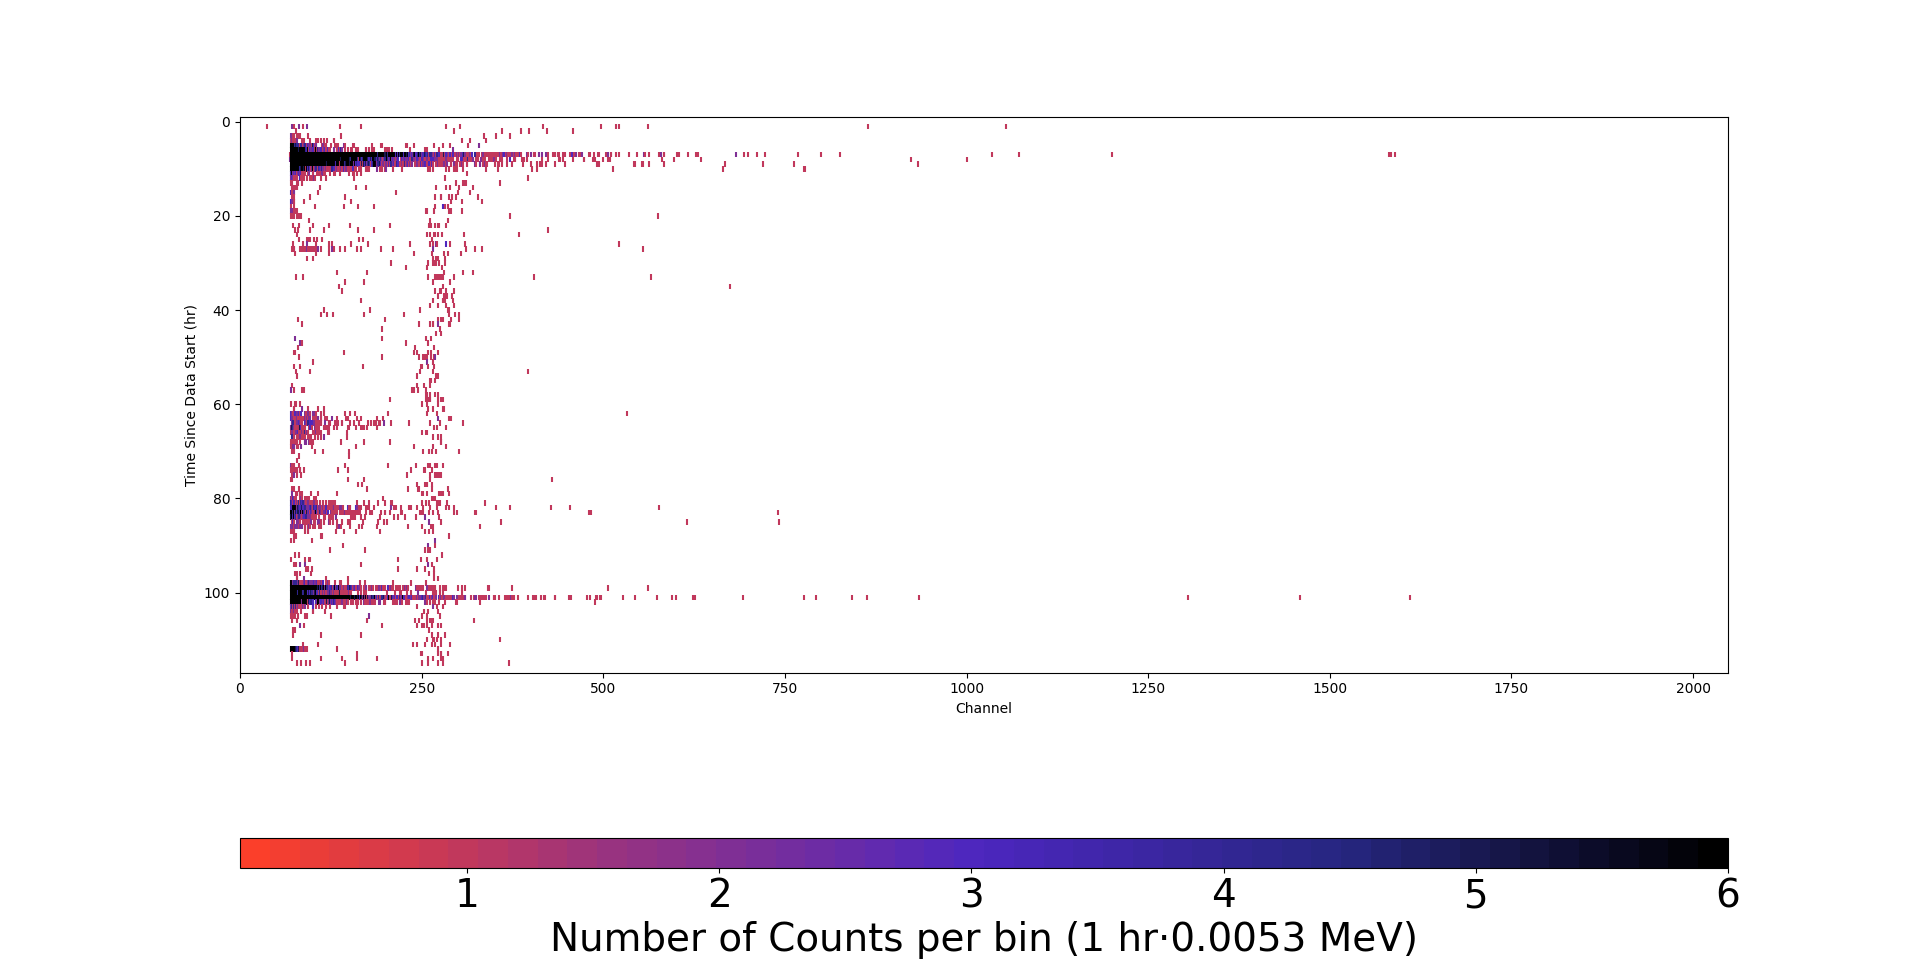
\includegraphics[width=0.9\textwidth]
            {assets/717/RD.png}
            \caption{Large regions of noisy data had to be removed}
        \end{center}
    \end{figure}
\end{frame}

\begin{frame}{Raw Data after Removing Bad Intervals, Run 717}
    \begin{figure}
        \begin{center}
            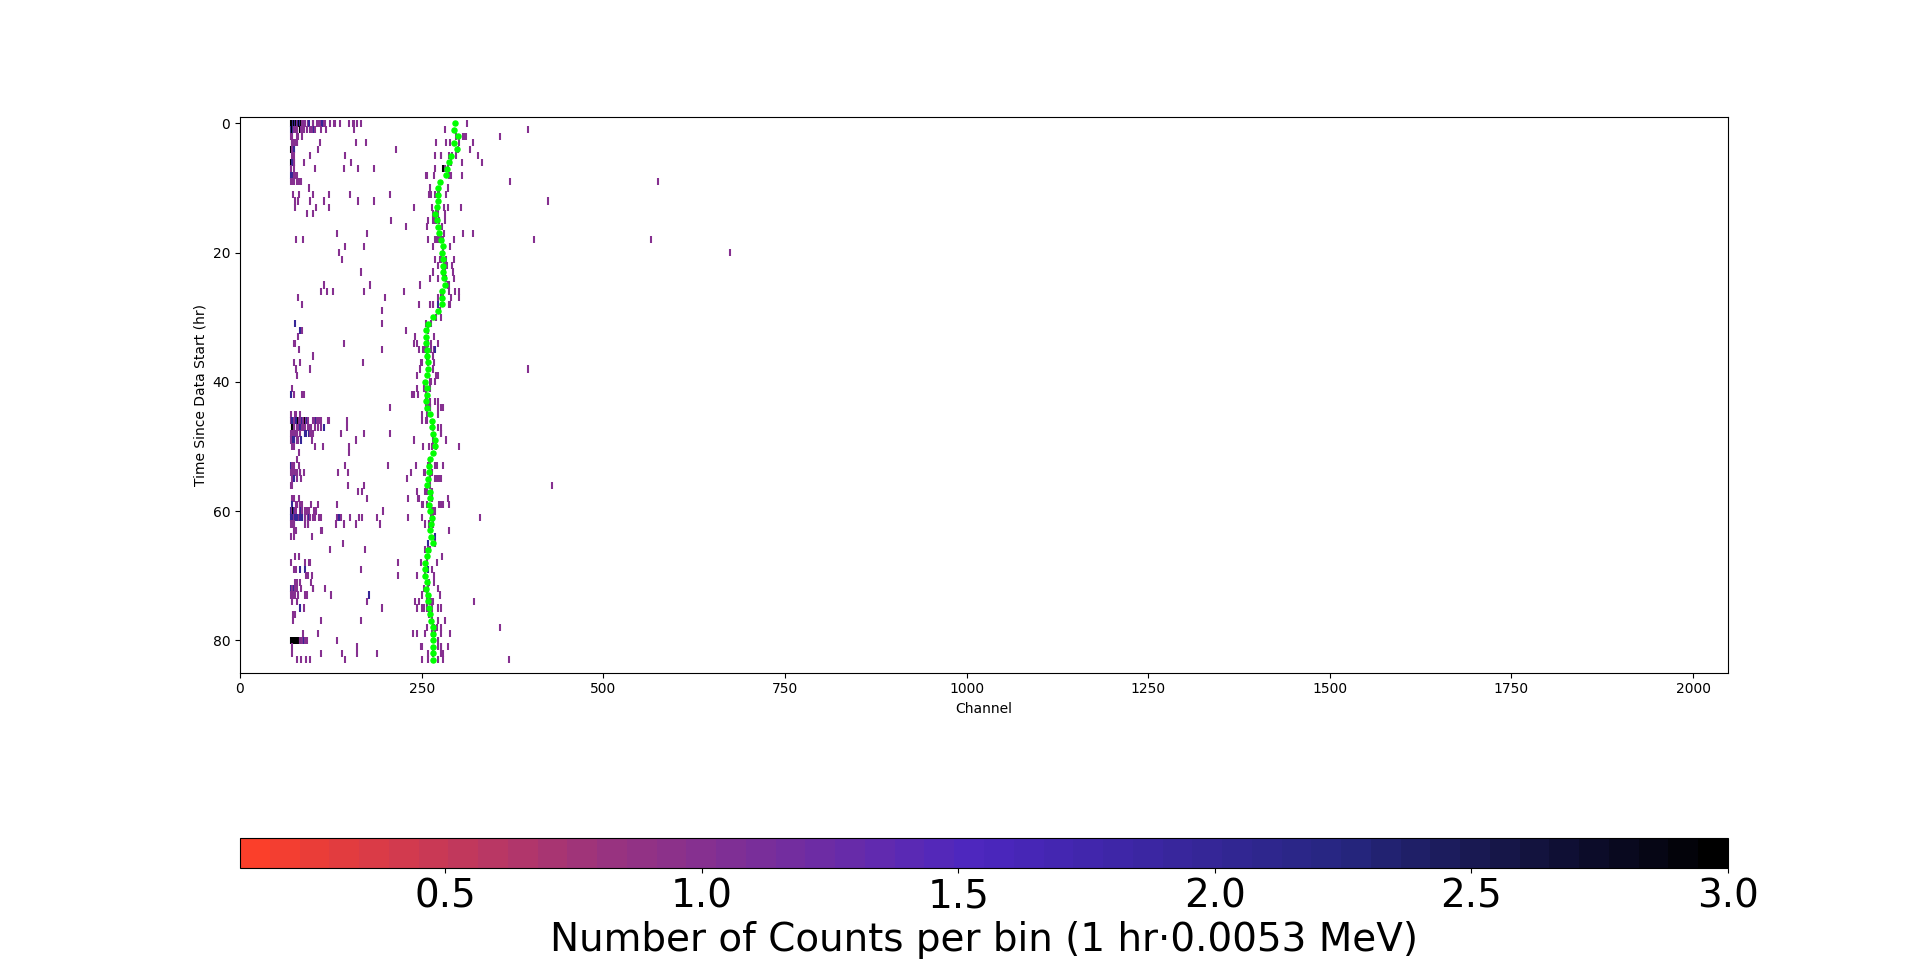
\includegraphics[width=0.9\textwidth]
            {assets/717/RDP.png}
            \caption{Gain is extremely low, resulting in poor data resolution}
        \end{center}
    \end{figure}
\end{frame}

\begin{frame}{Gain-Corrected Data, Run 717}
    \begin{figure}
        \begin{center}
            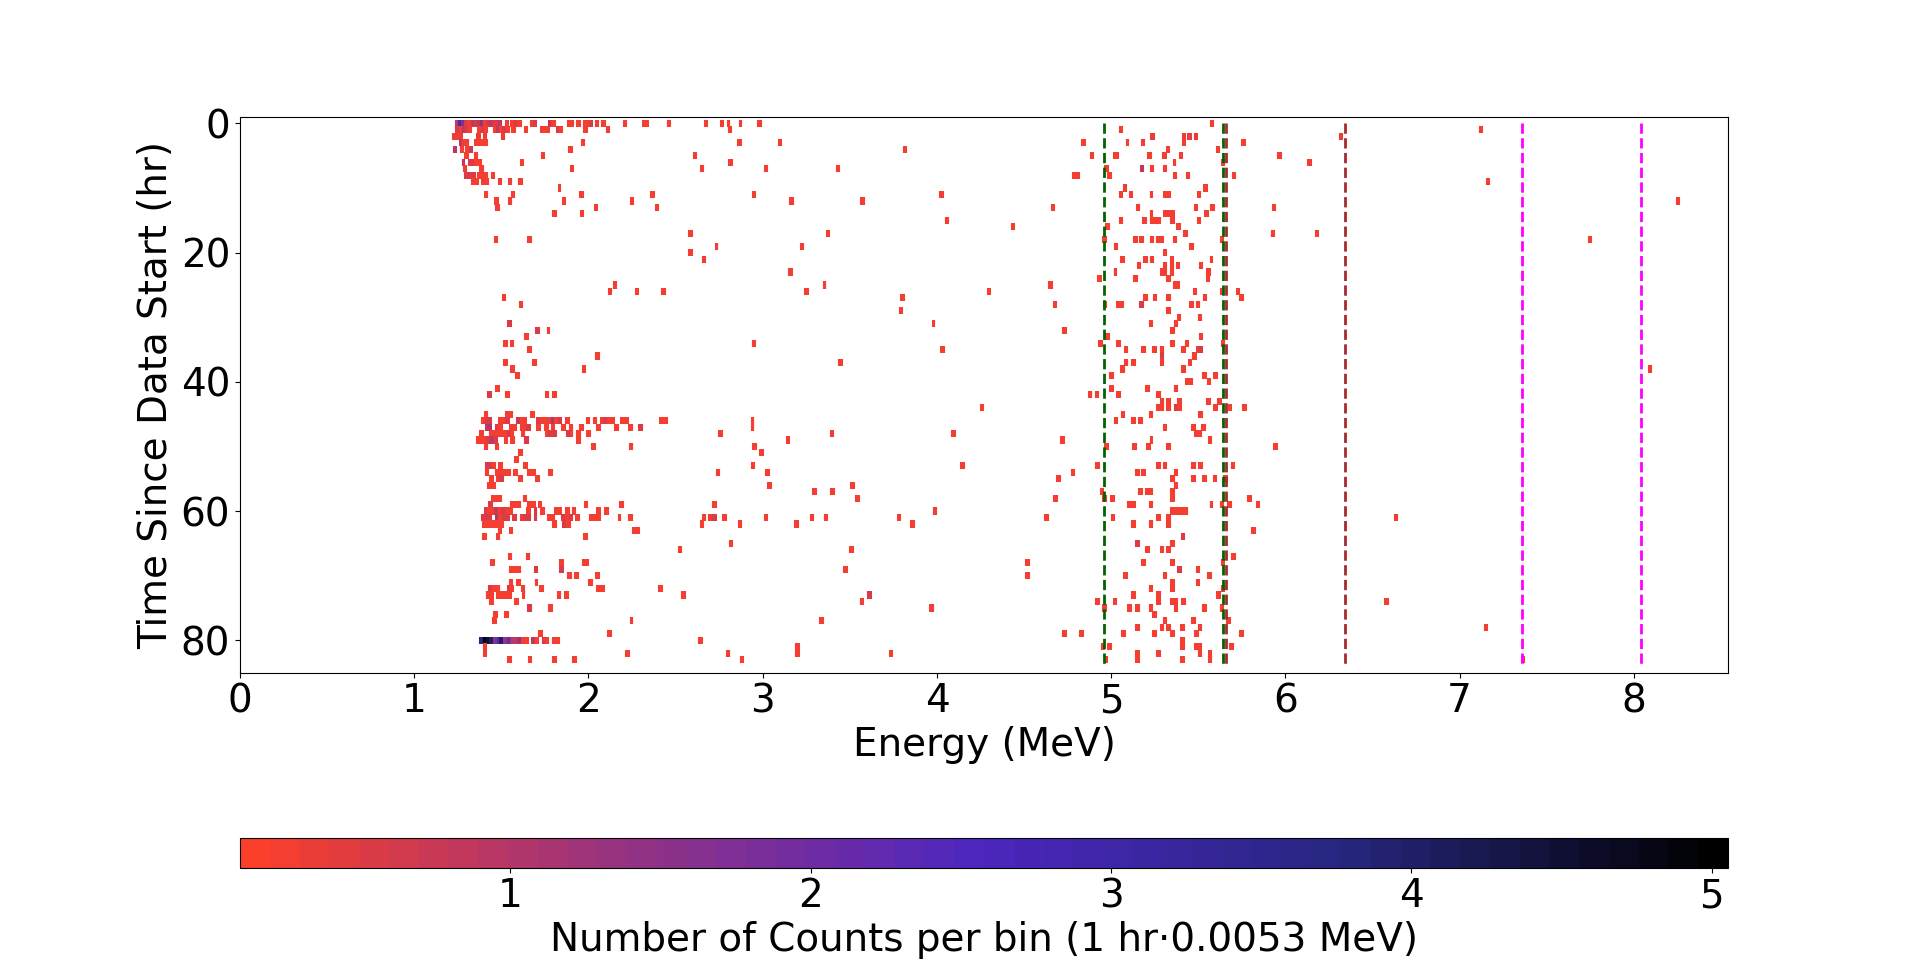
\includegraphics[width=0.9\textwidth]
            {assets/717/CD.png}
            \caption{Data has been corrected to center the 5.3 MeV $^{210}$Po peak at MCA channel 1000}
        \end{center}
    \end{figure}
\end{frame}

\begin{frame}{Counts vs. Energy, Run 717}
    \begin{figure}
        \begin{center}
            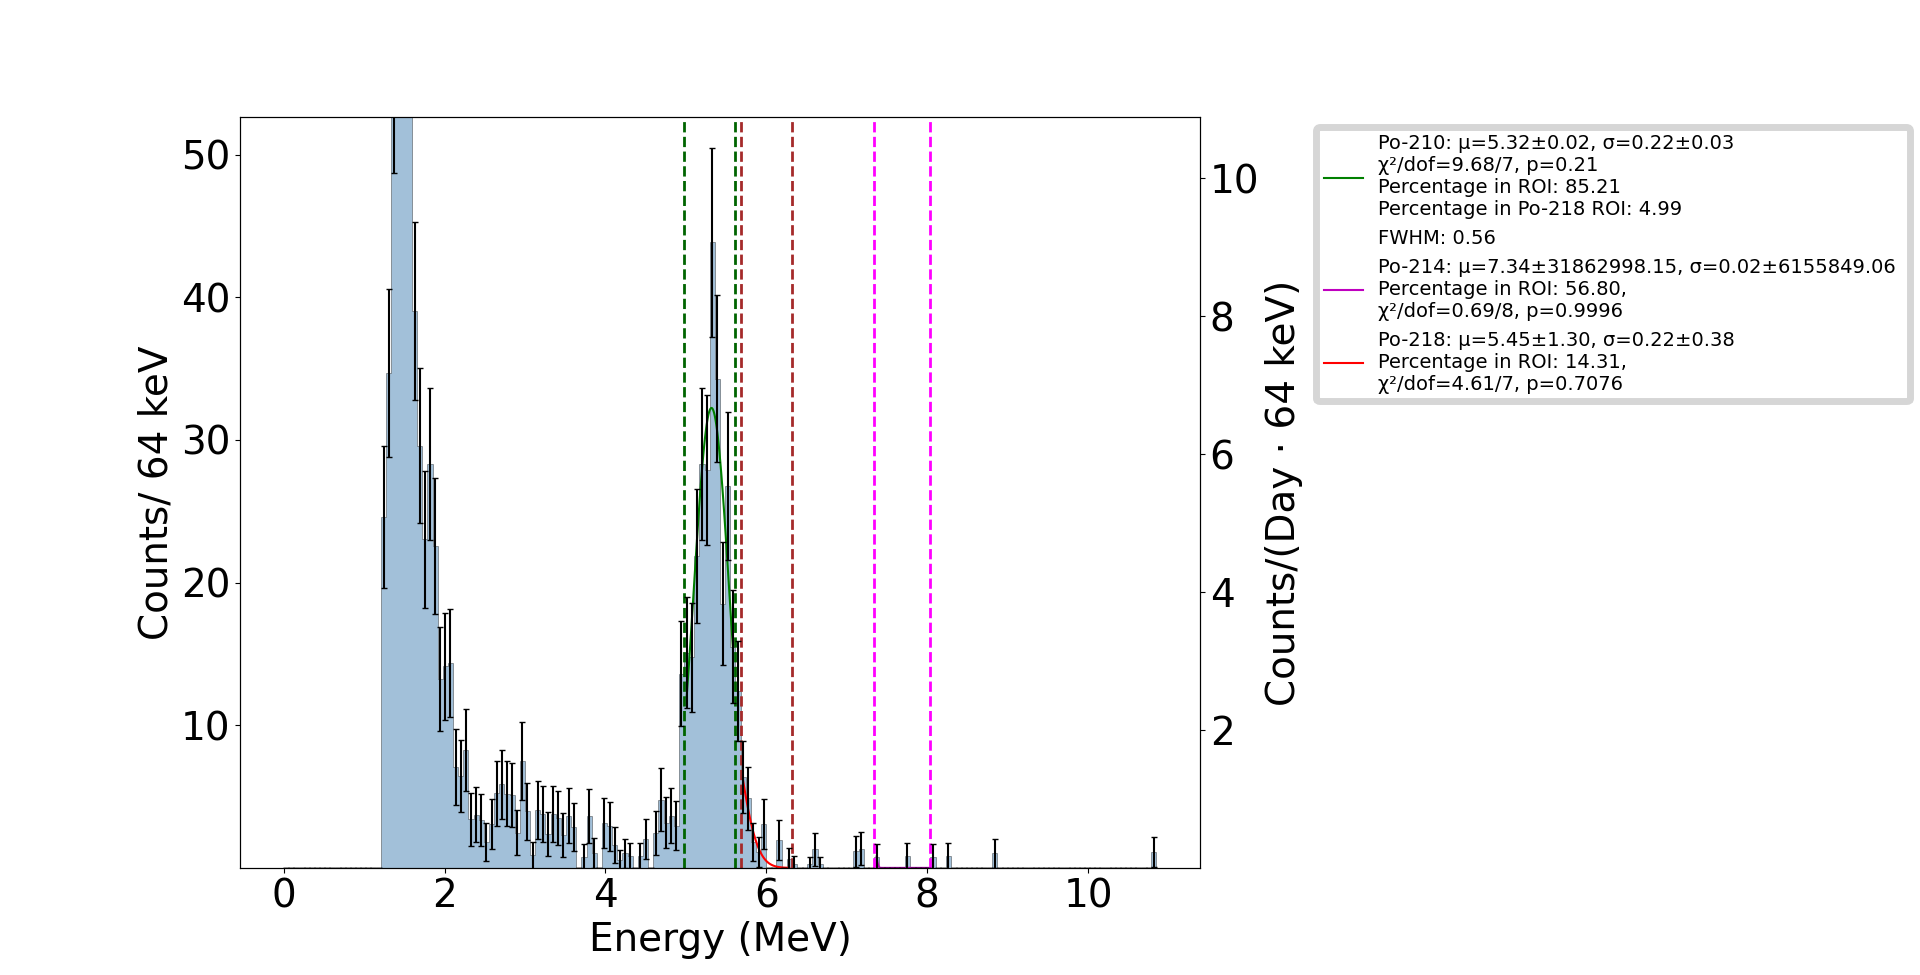
\includegraphics[width=0.9\textwidth]
            {assets/717/CvE.png}
            \caption{$^{210}$Po peak has poor resolution and bleeds into $^{218}$Po ROI}
        \end{center}
    \end{figure}
\end{frame}

\begin{frame}{Combined NLL, Run 717}
    \begin{figure}
        \begin{center}
            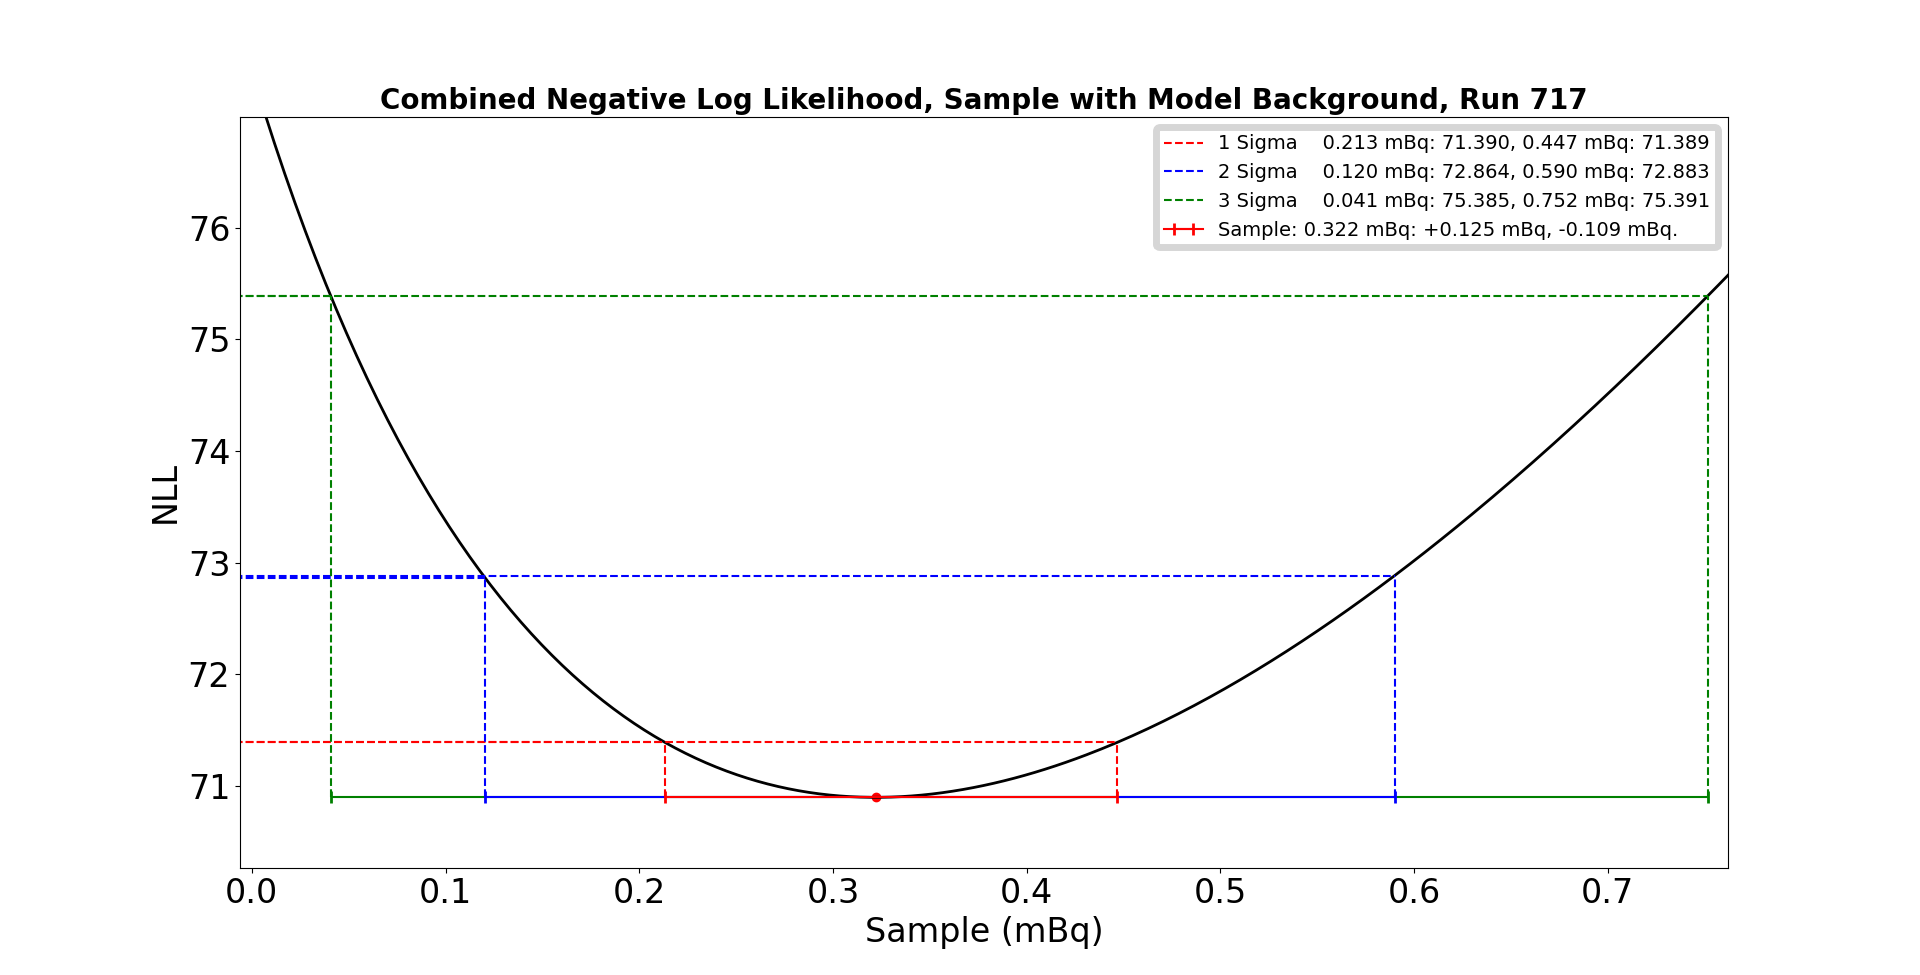
\includegraphics[width=0.9\textwidth]
            {assets/717/comNLL.png}
            \caption{This rate is not used because of the resolution problems discussed earlier}
        \end{center}
    \end{figure}
\end{frame}

\begin{frame}{$^{218}$Po NLL, Run 717}
    \begin{figure}
        \begin{center}
            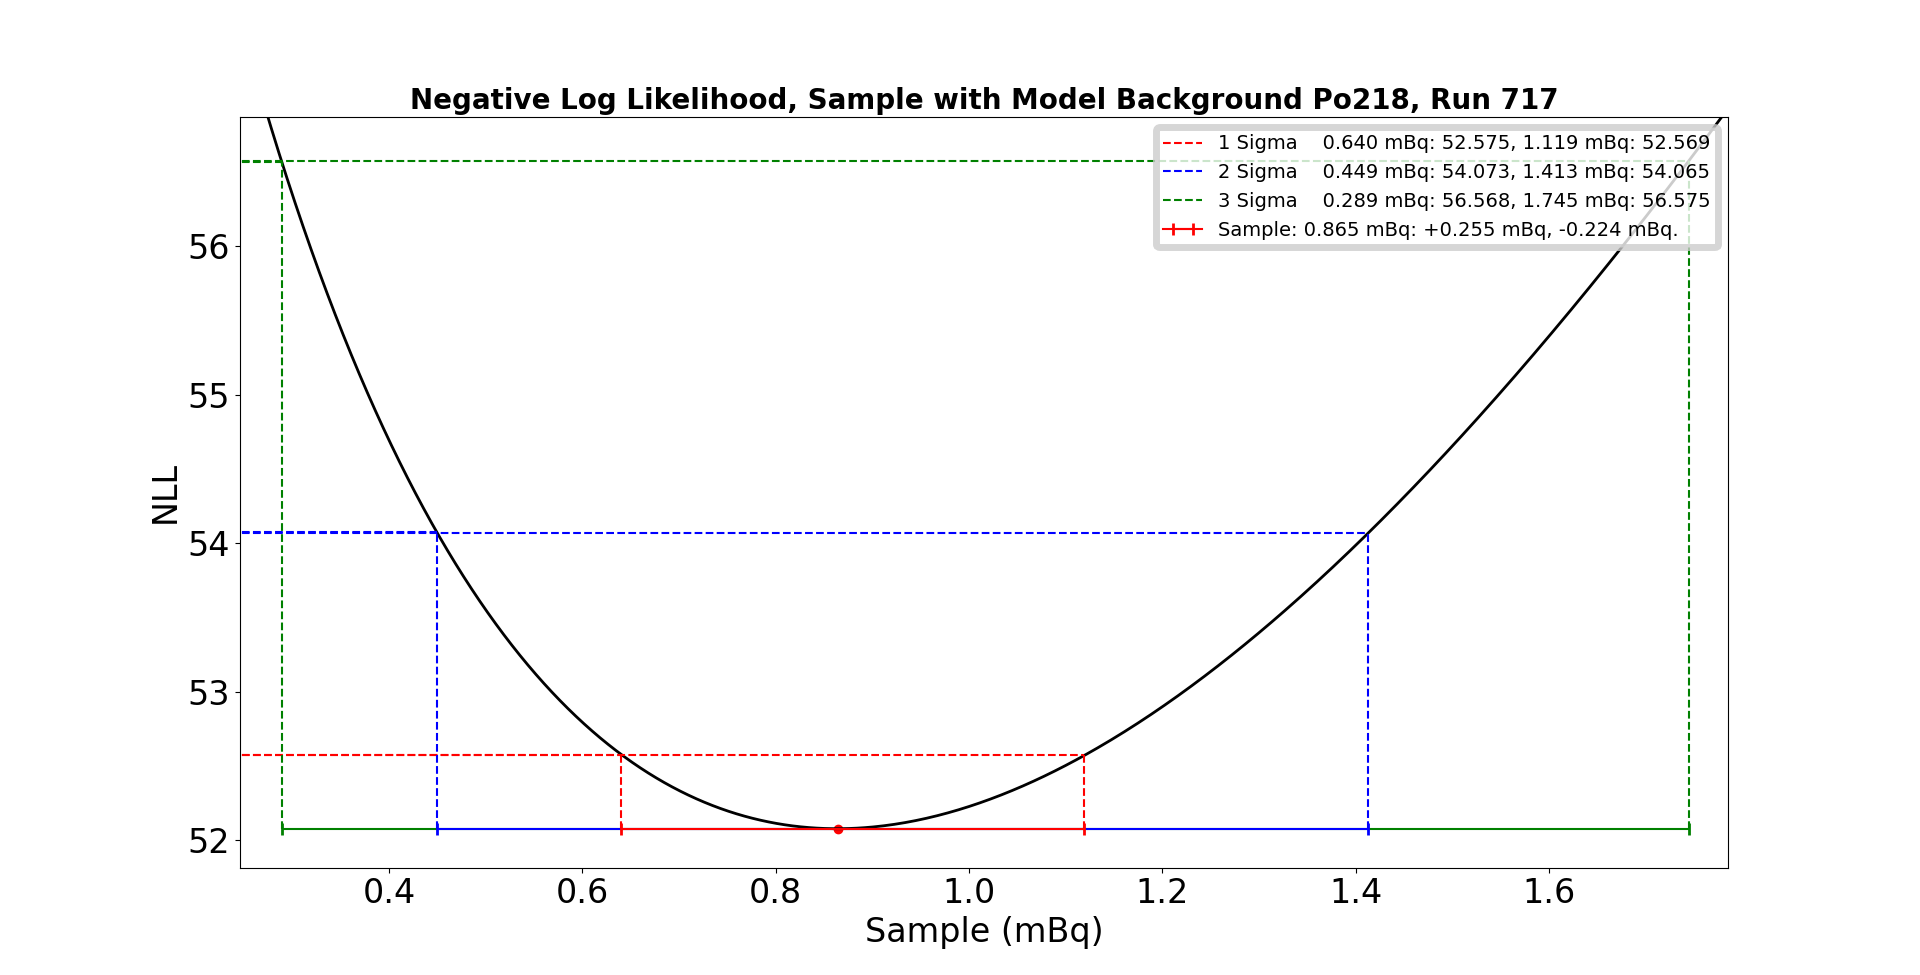
\includegraphics[width=0.9\textwidth]
            {assets/717/NLL218.png}
            \caption{This rate is artificially high because of spillage from the $^{210}$Po ROI}
        \end{center}
    \end{figure}
\end{frame}

\begin{frame}{$^{214}$Po NLL, Run 717}
    \begin{figure}
        \begin{center}
            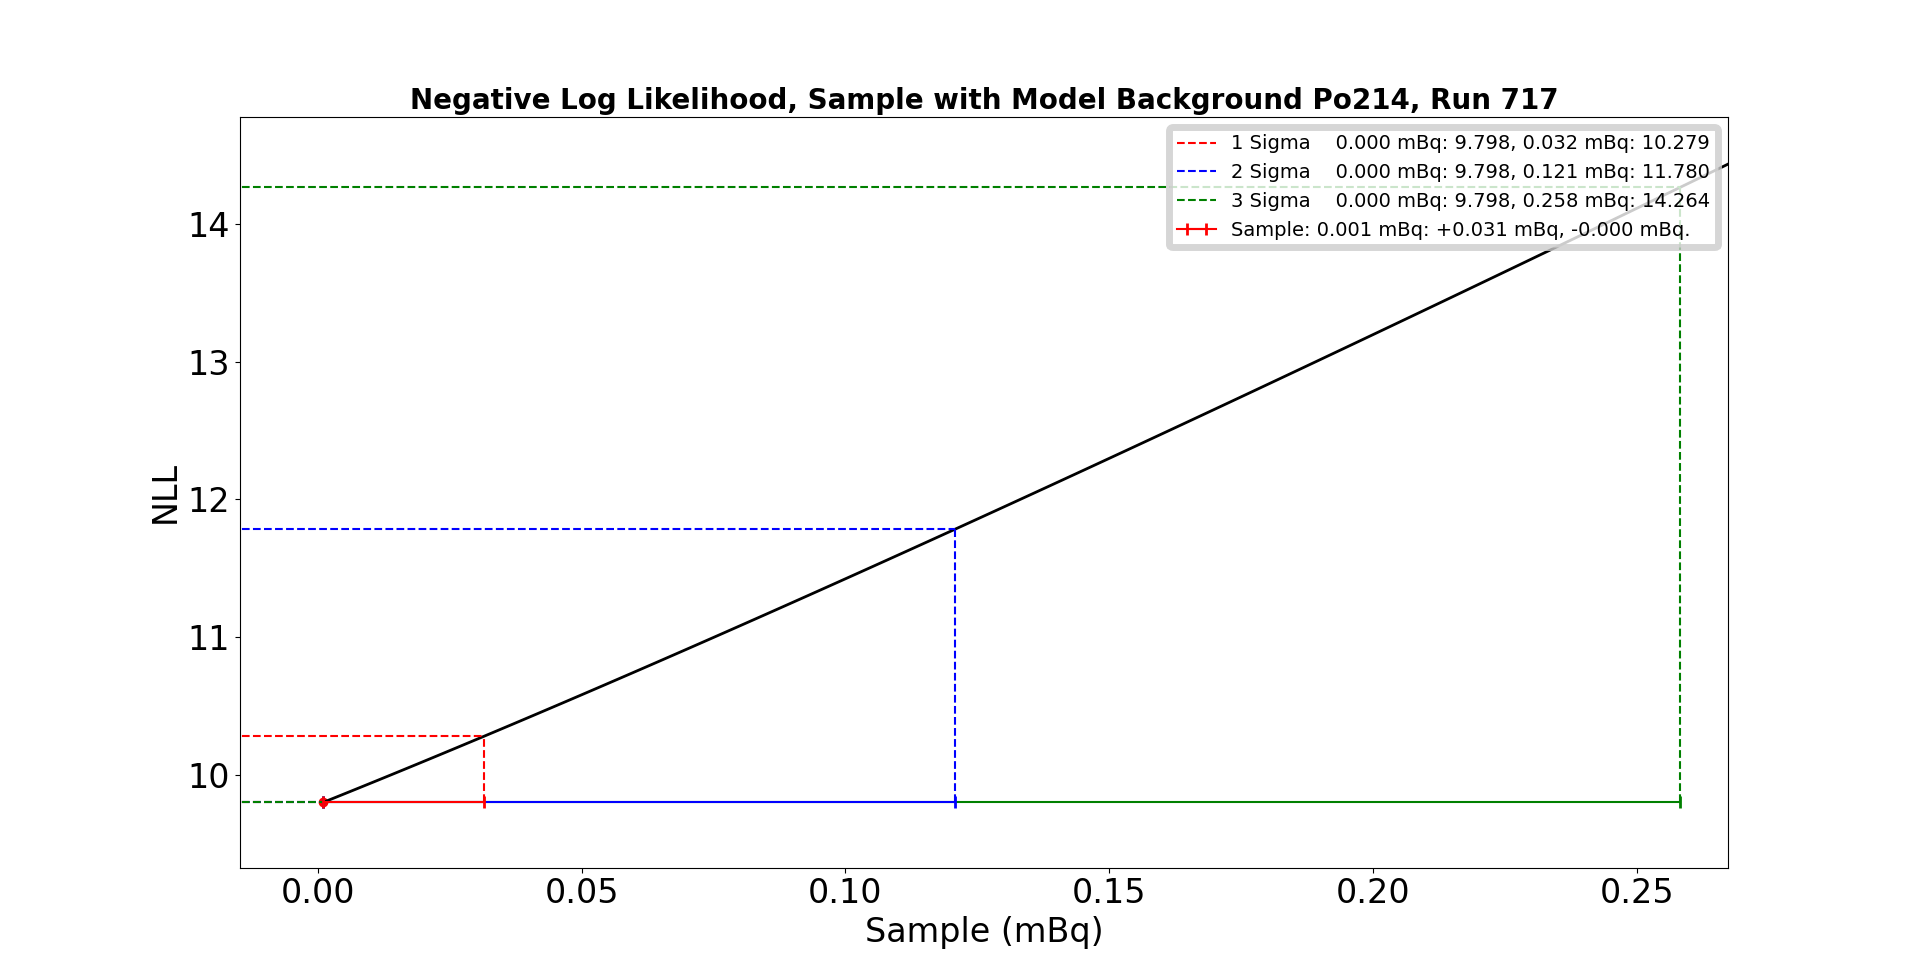
\includegraphics[width=0.9\textwidth]
            {assets/717/NLL214.png}
            \caption{This is the rate that was used to determine the emanation rate of Run 717}
        \end{center}
    \end{figure}
\end{frame}

\begin{frame}{Live Time Efficiency}
    \begin{figure}
        \begin{center}
            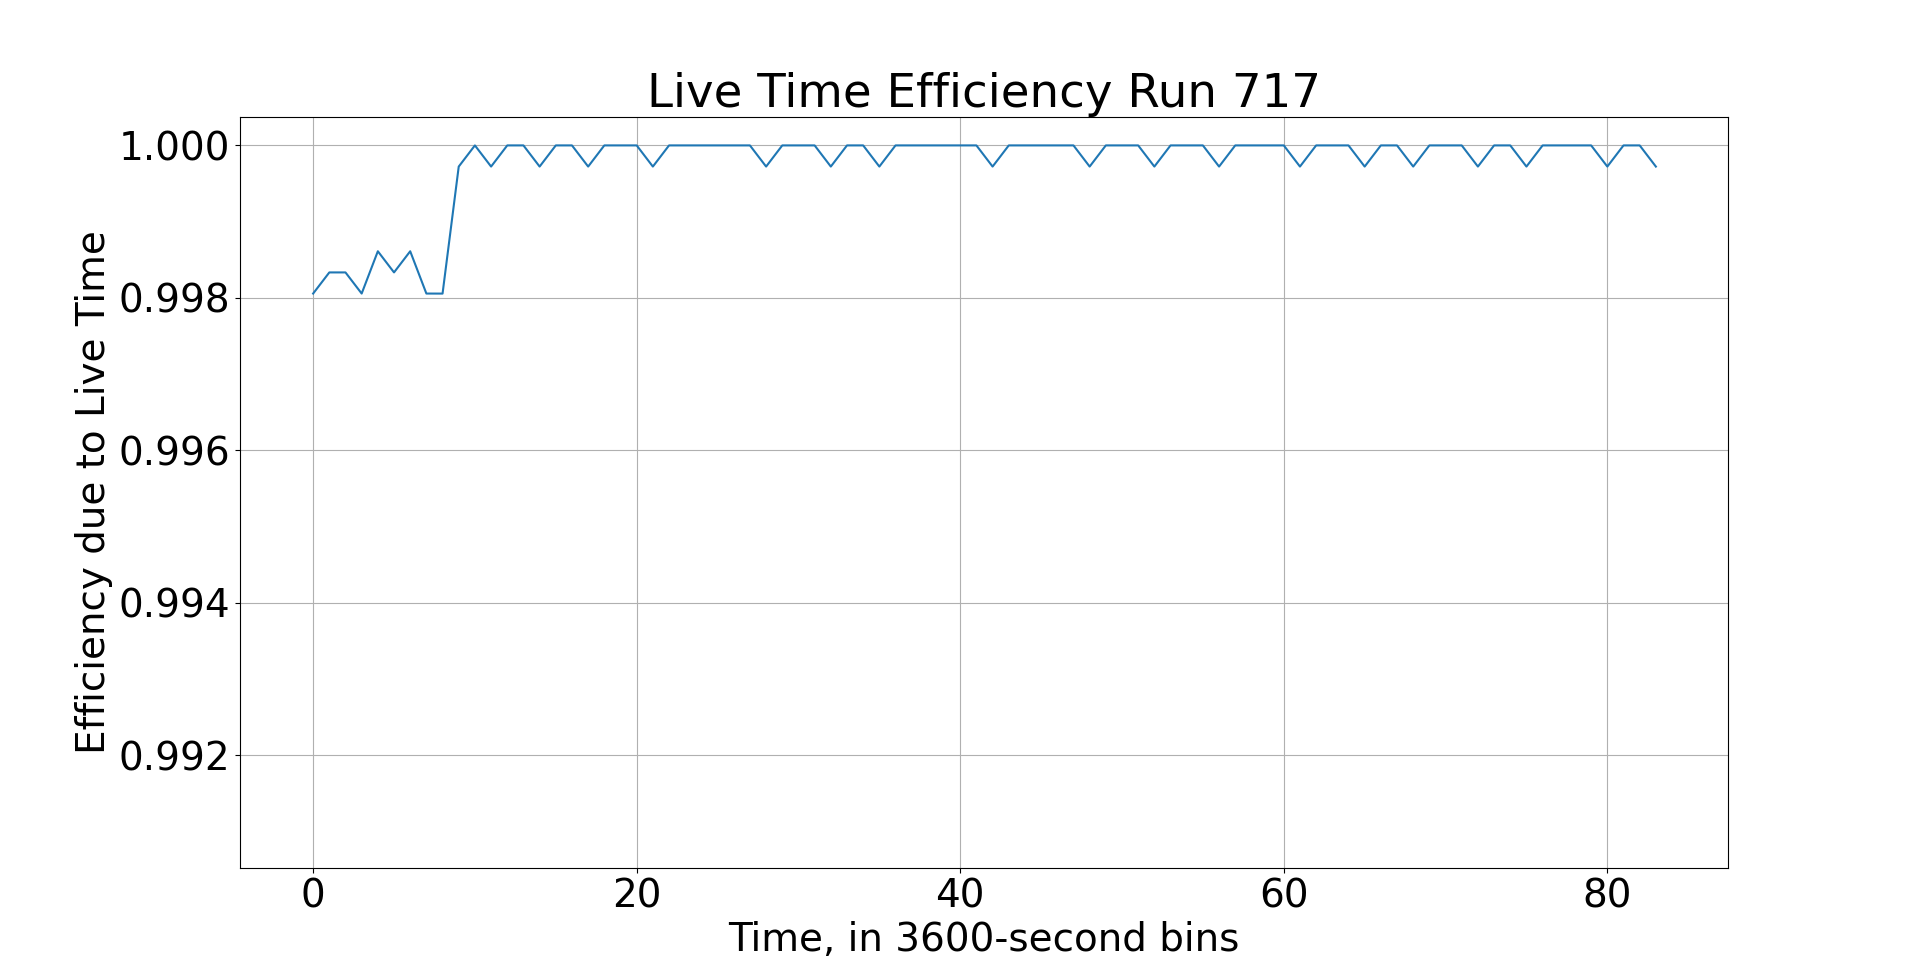
\includegraphics[width=0.9\textwidth]
            {assets/717/LTE.png}
            \caption{Detector had relatively little dead time}
        \end{center}
    \end{figure}
\end{frame}

\begin{frame}{Notes on Run 717 Analysis}
    A large portion of the data had to be discarded due to high levels of noise that interfered
    with gain correction and rate finding.
    The run also exhibited low gain, with the $^{210}$Po peak resting somewhere around MCA channel
    250, rather than the standard 1000.
    The low gain caused further issues with data resolution, which caused the $^{218}$Po rate calculated
    to include spill-over from $^{210}$Po events.
    Because of this, the $^{214}$Po rate was exclusively used to determine the emanation rate for this run.

    \hyperlink{RvT_717}{\beamerbutton{Back to Rate vs Time Run 717}}
\end{frame}

\begin{frame}{Run 720 Backup Slides}
\label{720_Backup}
    The following slides contain additional data and information regarding Run 720.
\end{frame}

\begin{frame}{Raw Data, Run 720}
    \begin{figure}
        \begin{center}
            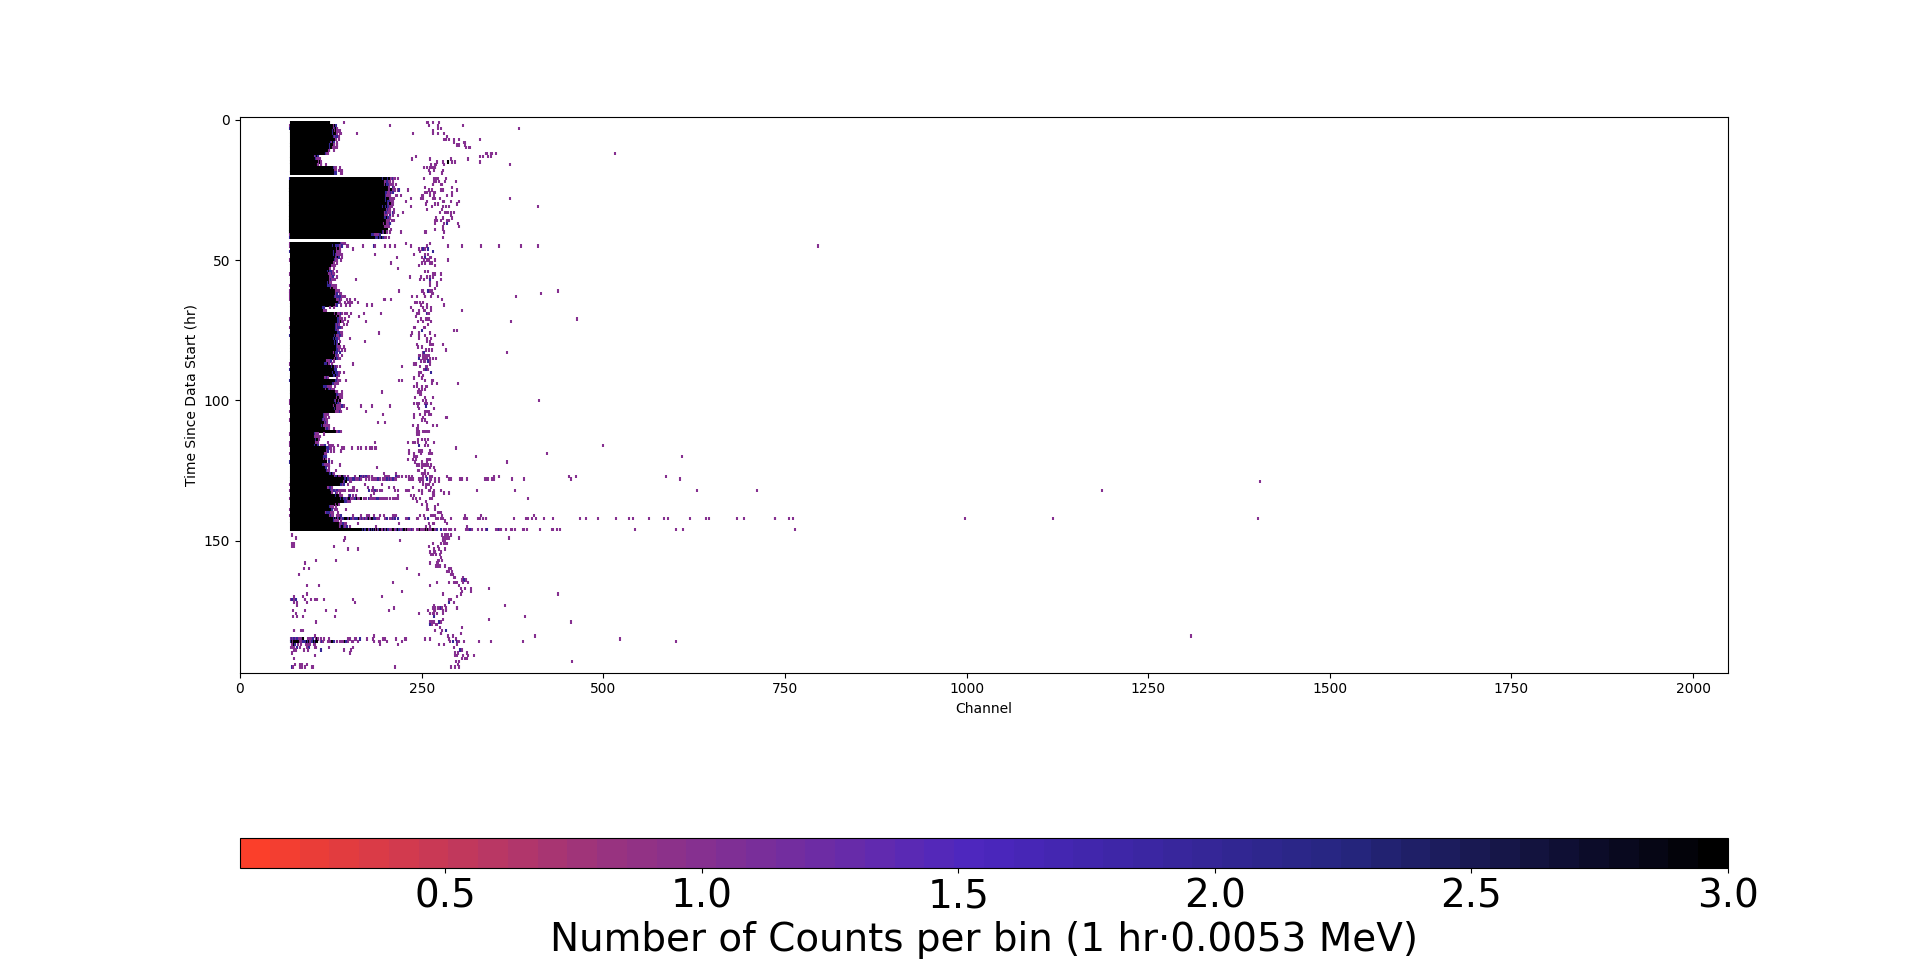
\includegraphics[width=0.9\textwidth]
            {assets/720/RD.png}
            \caption{Run 720 exhibited both gain shift and areas of problematic noise}
        \end{center}
    \end{figure}
\end{frame}

\begin{frame}{Raw Data after Removing Bad Intervals, Run 720}
    \begin{figure}
        \begin{center}
            \includegraphics[width=0.9\textwidth]
            {assets/720/RDP.png}
            \caption{Gain is extremely low, resulting in poor data resolution}
        \end{center}
    \end{figure}
\end{frame}

\begin{frame}{Gain-Corrected Data, Run 720}
    \begin{figure}
        \begin{center}
            \includegraphics[width=0.9\textwidth]
            {assets/720/CD.png}
            \caption{Data has been corrected to center the 5.3 MeV $^{210}$Po peak at MCA channel 1000}
        \end{center}
    \end{figure}
\end{frame}

\begin{frame}{Counts vs. Energy, Run 720}
    \begin{figure}
        \begin{center}
            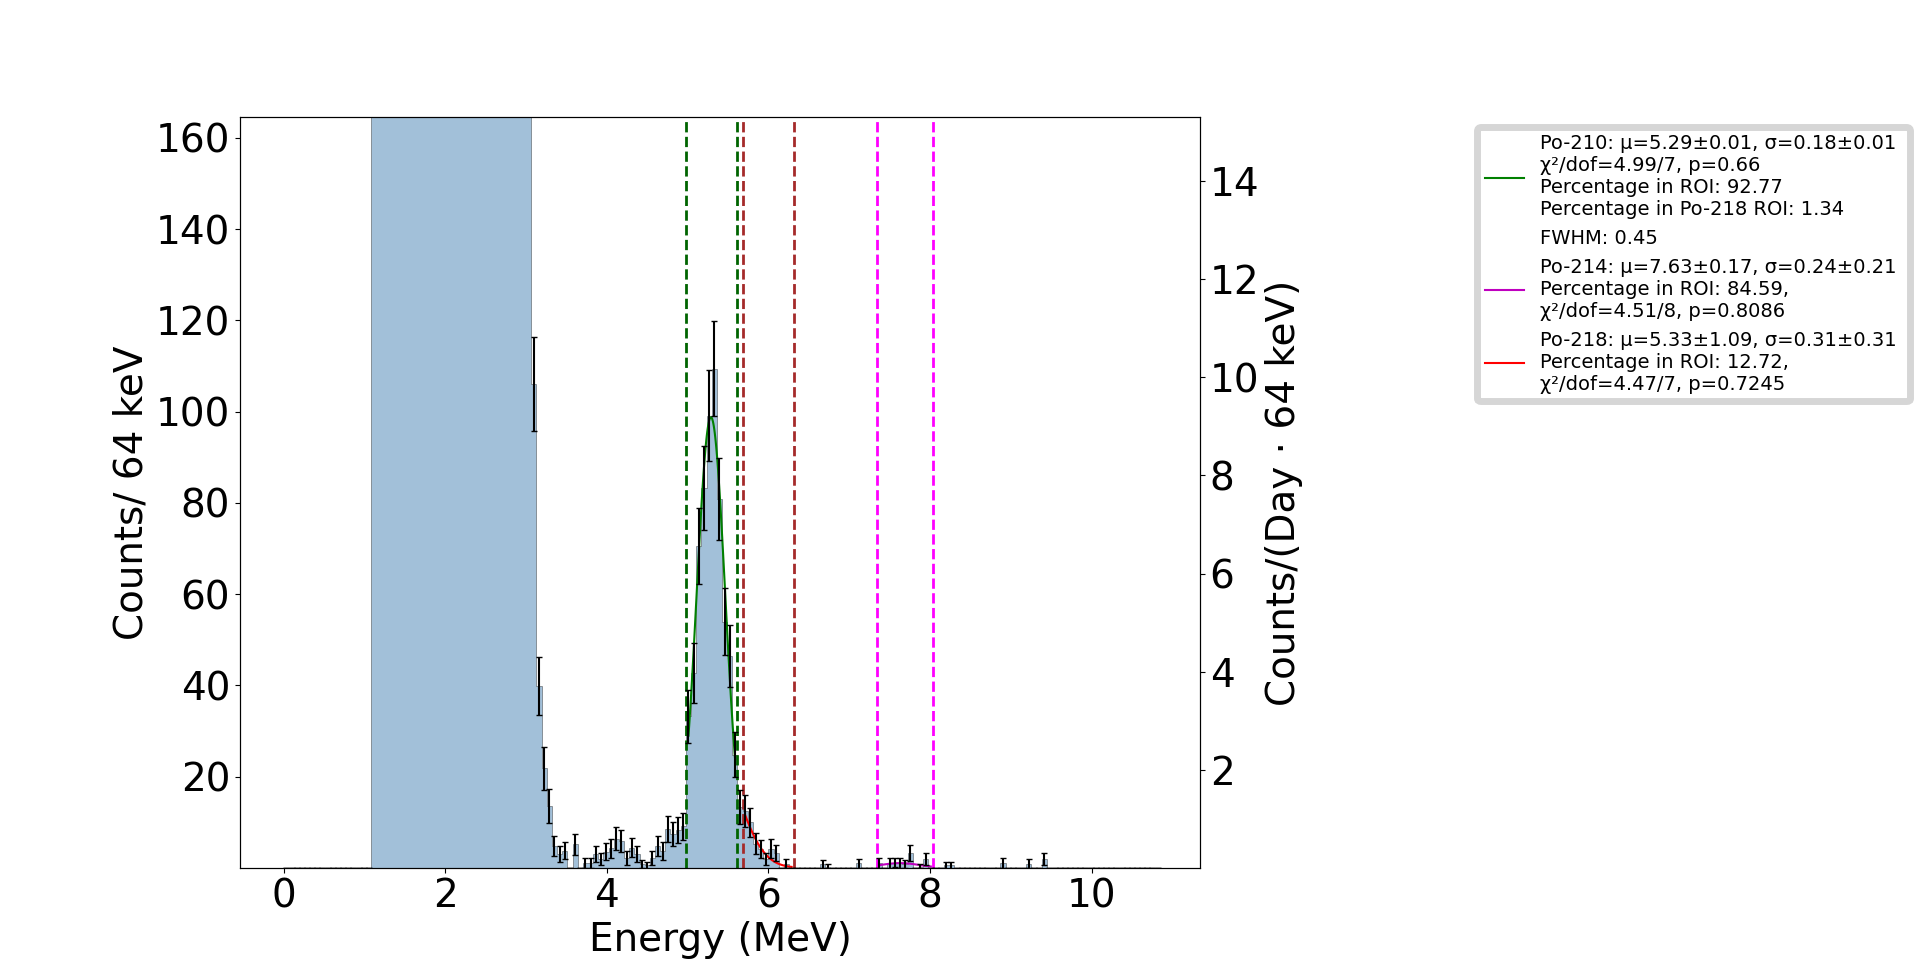
\includegraphics[width=0.9\textwidth]
            {assets/720/CvE.png}
            \caption{$^{210}$Po peak has poor resolution and bleeds into $^{218}$Po ROI}
        \end{center}
    \end{figure}
\end{frame}

\begin{frame}{Combined NLL, Run 720}
    \begin{figure}
        \begin{center}
            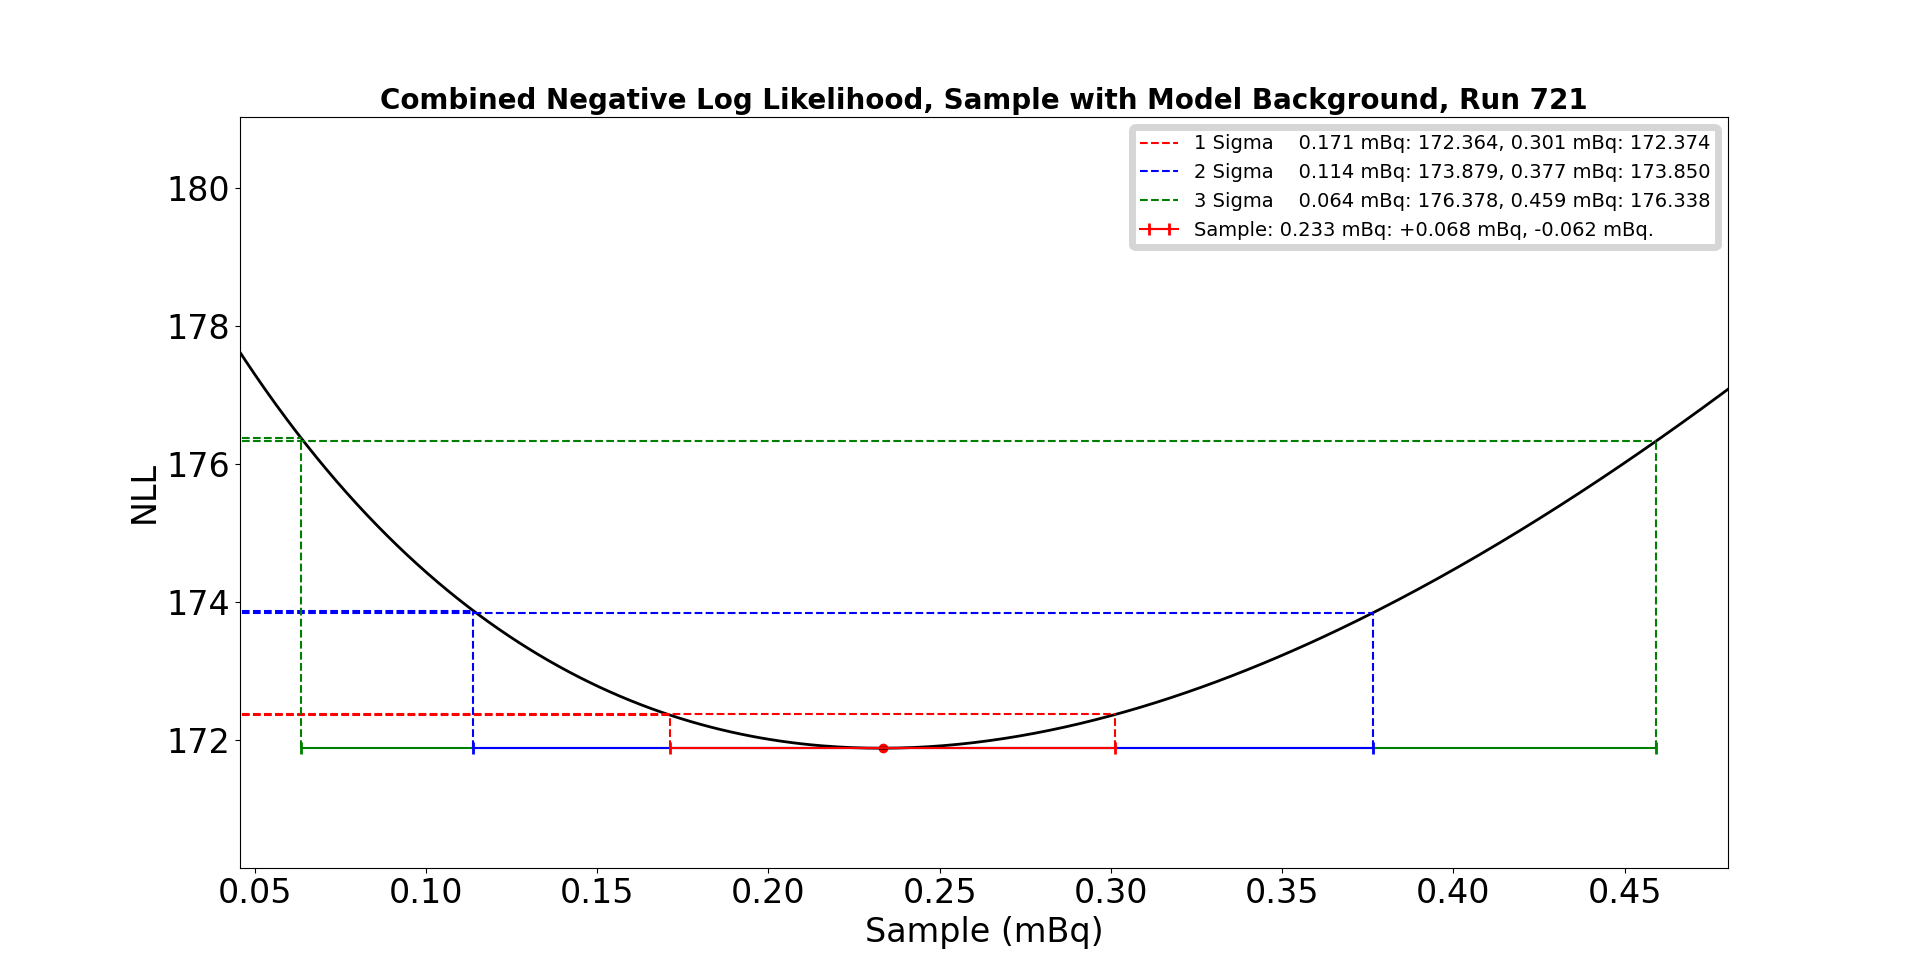
\includegraphics[width=0.9\textwidth]
            {assets/720/comNLL.png}
            \caption{This rate is not used because of the resolution problems discussed earlier}
        \end{center}
    \end{figure}
\end{frame}

\begin{frame}{$^{218}$Po NLL, Run 720}
    \begin{figure}
        \begin{center}
            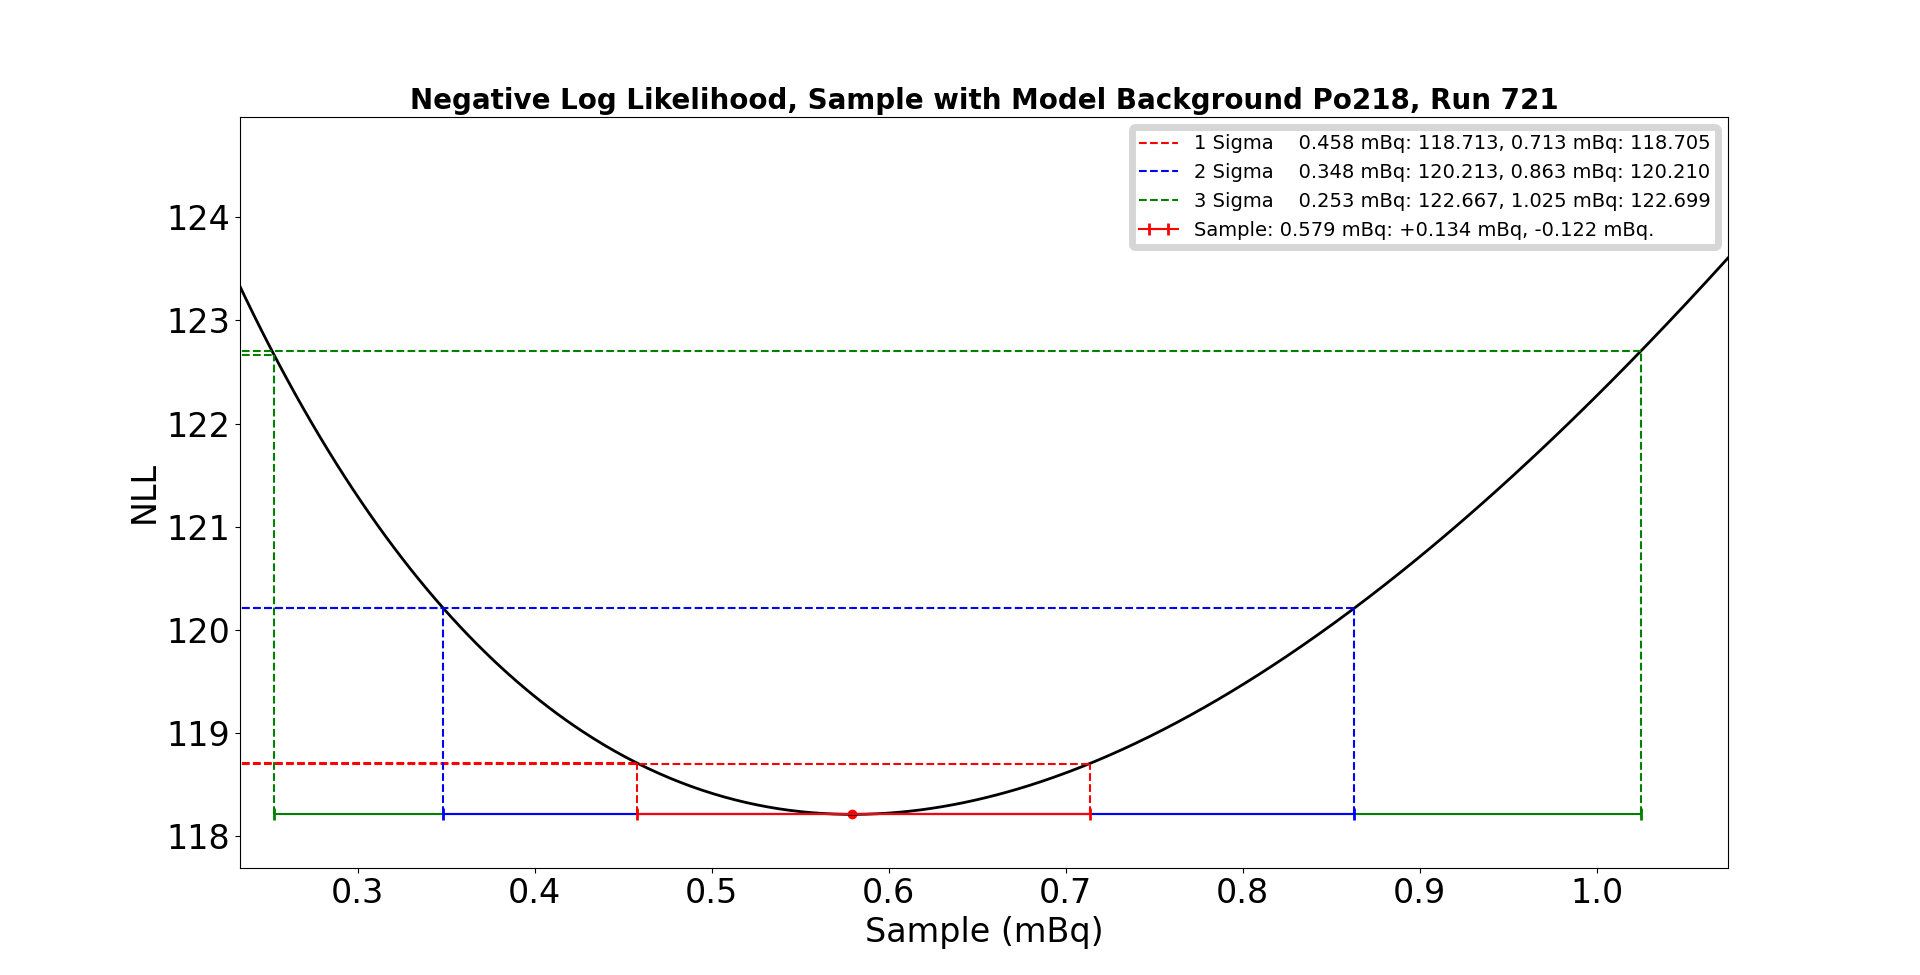
\includegraphics[width=0.9\textwidth]
            {assets/720/NLL218.png}
            \caption{This rate is artificially high because of spillage from the $^{210}$Po ROI}
        \end{center}
    \end{figure}
\end{frame}

\begin{frame}{$^{214}$Po NLL, Run 720}
    \begin{figure}
        \begin{center}
            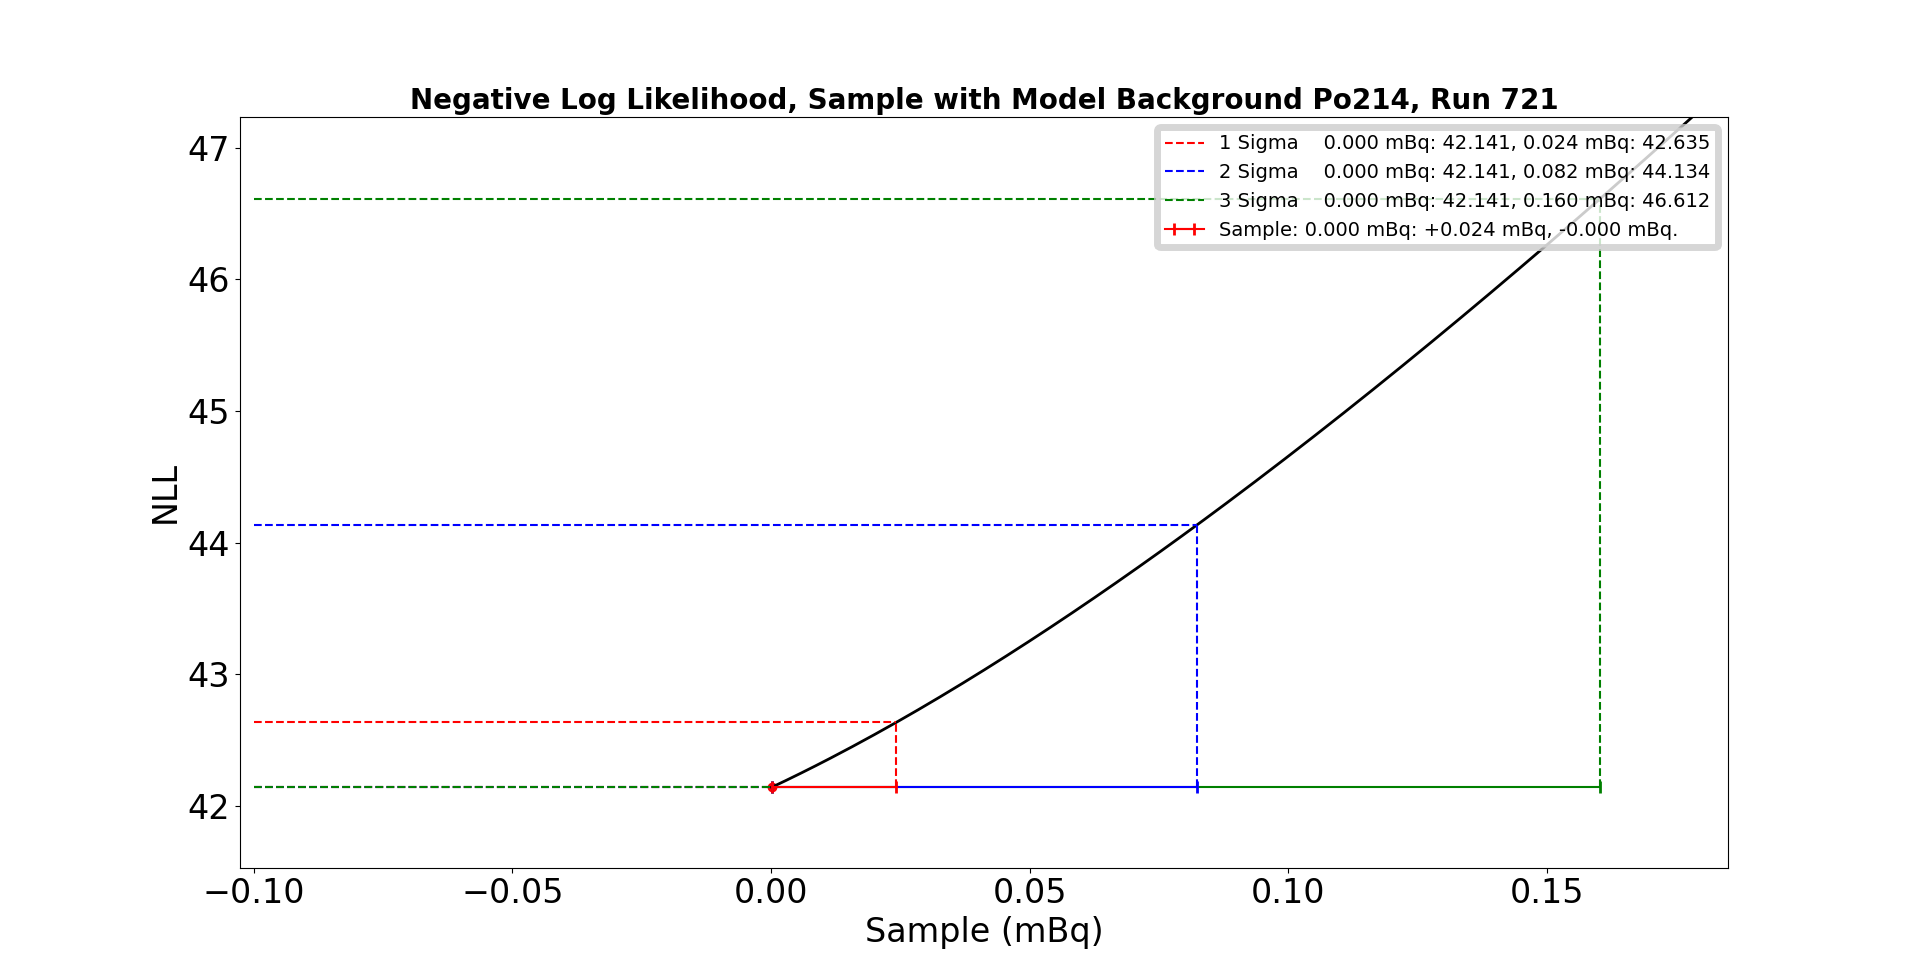
\includegraphics[width=0.9\textwidth]
            {assets/720/NLL214.png}
            \caption{This is the rate that was used to determine the emanation rate of Run 720}
        \end{center}
    \end{figure}
\end{frame}

\begin{frame}{Live Time Efficiency}
    \begin{figure}
        \begin{center}
            \includegraphics[width=0.9\textwidth]
            {assets/720/LTE.png}
            \caption{Detector had relatively little dead time}
        \end{center}
    \end{figure}
\end{frame}

\begin{frame}{Notes on Run 721 Analysis}
    Run 721 exhibits low gain that appears to vary periodically.
    Unfortunately, there is no environmental data to compare the shifts to.
    Several bins had to be cut due to high noise.
    The low resolution exhibited by Run 721 gives way to $^{210}$Po events spilling over
    into the $^{218}$Po ROI.
    Because of this, the $^{214}$Po rate alone was used to determine the emanation rate
    for run 721.
    Overall, Run 721 appears to be consistent with our backgrounds.

    \hyperlink{RvT_721}{\beamerbutton{Back to Rate vs Time Run 721}}
\end{frame}

\begin{frame}{Run 721 Backup Slides}
\label{721_Backup}
    The following slides contain additional data and information regarding Run 721.
\end{frame}

\begin{frame}{Raw Data, Run 721}
    \begin{figure}
        \begin{center}
            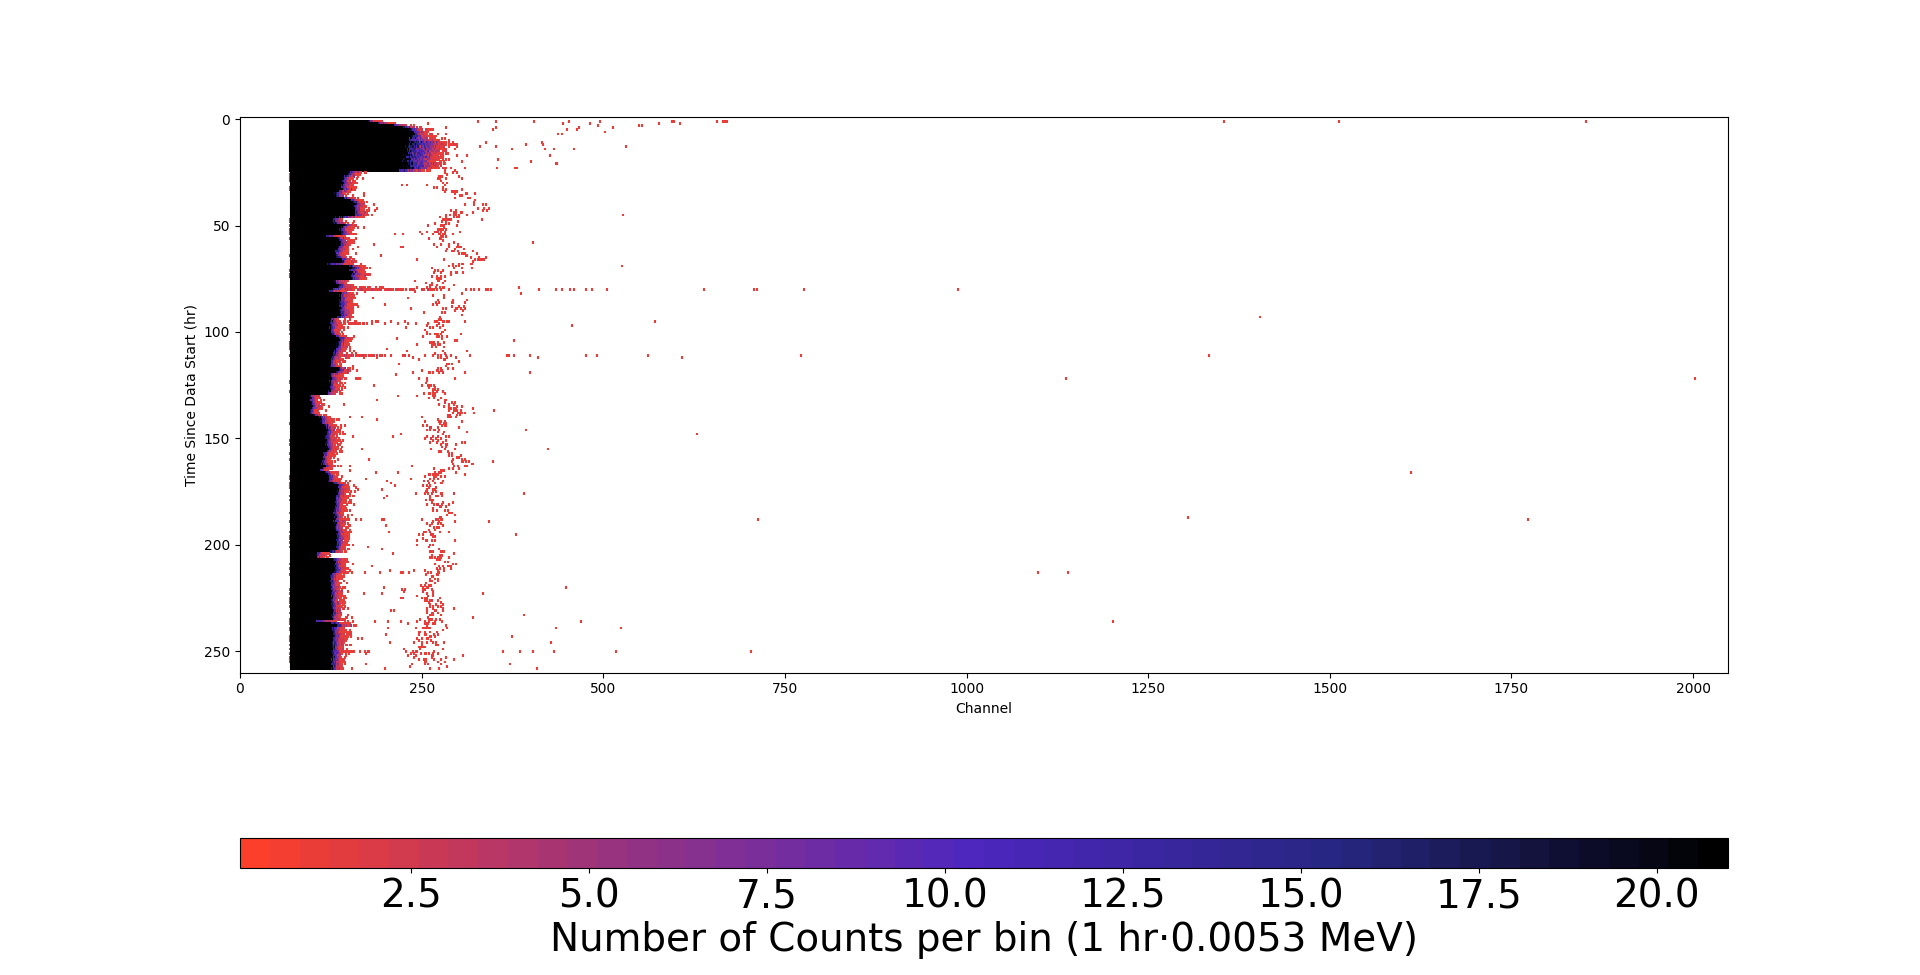
\includegraphics[width=0.9\textwidth]
            {assets/721/RD.png}
            \caption{Run 721 exhibited both gain shift and areas of problematic noise}
        \end{center}
    \end{figure}
\end{frame}

\begin{frame}{Raw Data after Removing Bad Intervals, Run 721}
    \begin{figure}
        \begin{center}
            \includegraphics[width=0.9\textwidth]
            {assets/721/RDP.png}
            \caption{Gain is extremely low, resulting in poor data resolution}
        \end{center}
    \end{figure}
\end{frame}

\begin{frame}{Gain-Corrected Data, Run 721}
    \begin{figure}
        \begin{center}
            \includegraphics[width=0.9\textwidth]
            {assets/721/CD.png}
            \caption{Data has been corrected to center the 5.3 MeV $^{210}$Po peak at MCA channel 1000}
        \end{center}
    \end{figure}
\end{frame}

\begin{frame}{Counts vs. Energy, Run 721}
    \begin{figure}
        \begin{center}
            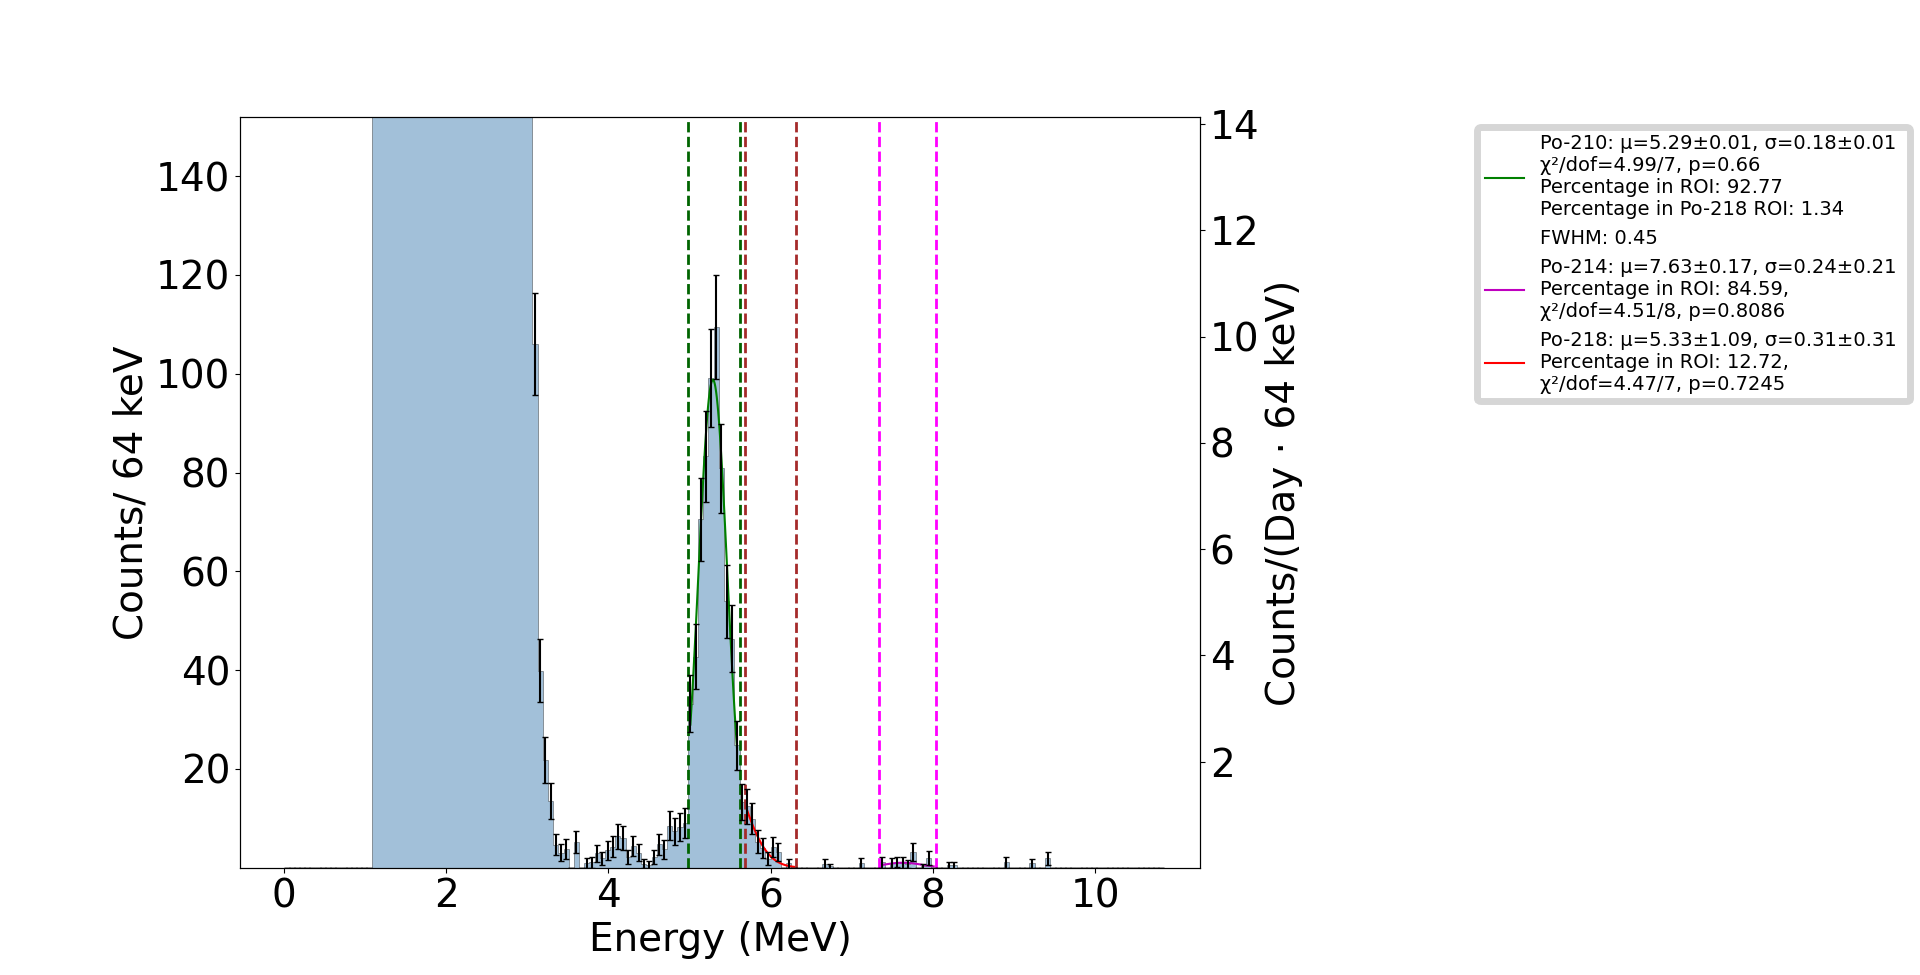
\includegraphics[width=0.9\textwidth]
            {assets/721/CvE.png}
            \caption{$^{210}$Po peak has poor resolution and bleeds into $^{218}$Po ROI}
        \end{center}
    \end{figure}
\end{frame}

\begin{frame}{Combined NLL, Run 721}
    \begin{figure}
        \begin{center}
            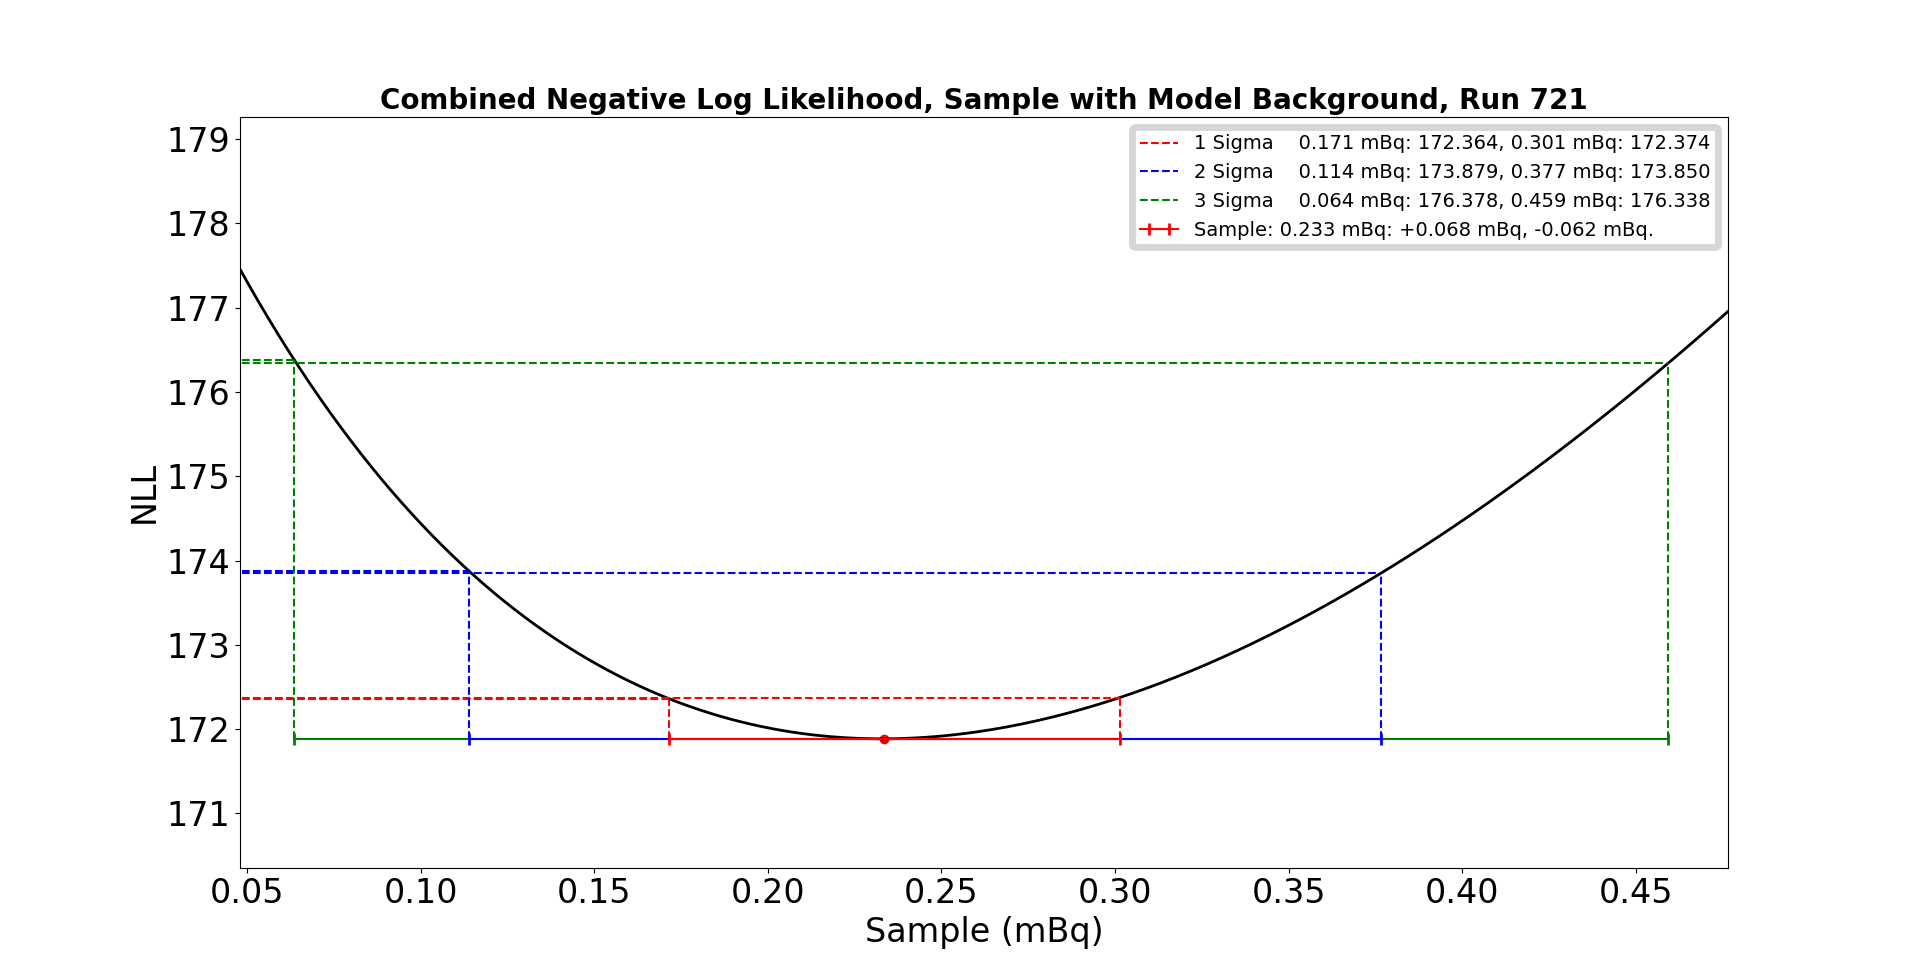
\includegraphics[width=0.9\textwidth]
            {assets/721/comNLL.png}
            \caption{This rate is not used because of the resolution problems discussed earlier}
        \end{center}
    \end{figure}
\end{frame}

\begin{frame}{$^{218}$Po NLL, Run 721}
    \begin{figure}
        \begin{center}
            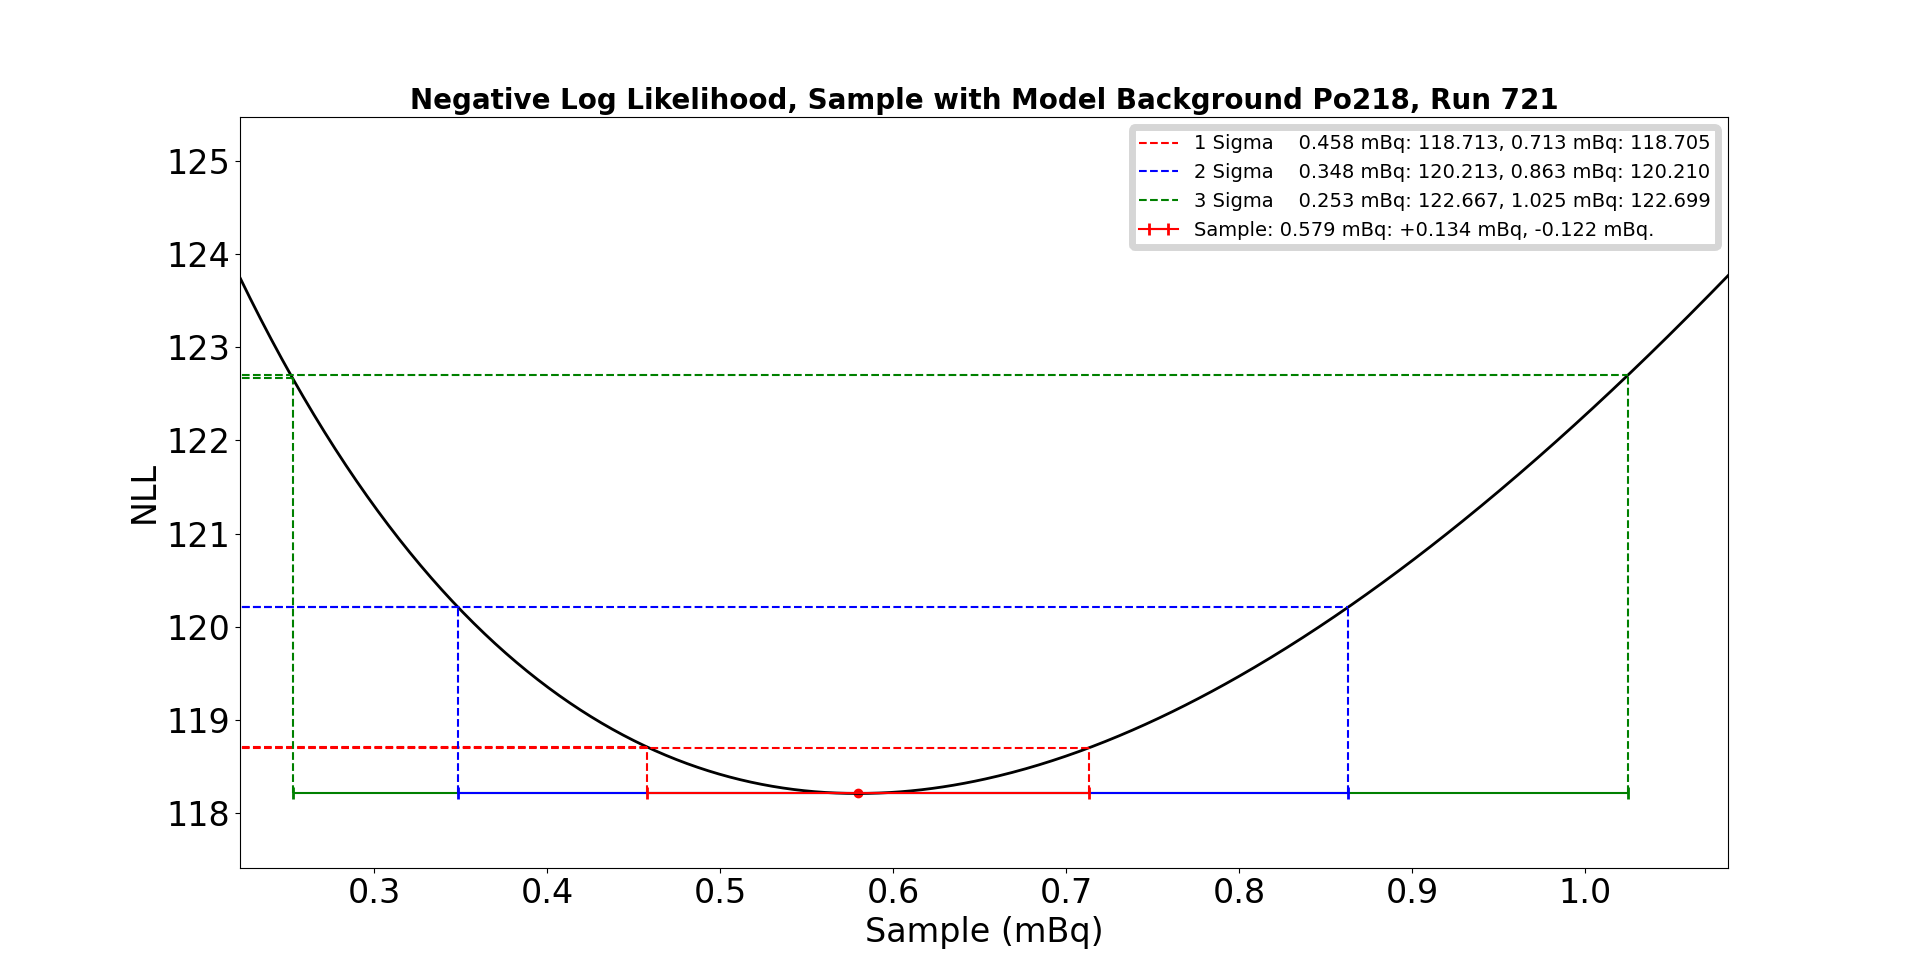
\includegraphics[width=0.9\textwidth]
            {assets/721/NLL218.png}
            \caption{This rate is artificially high because of spillage from the $^{210}$Po ROI}
        \end{center}
    \end{figure}
\end{frame}

\begin{frame}{$^{214}$Po NLL, Run 721}
    \begin{figure}
        \begin{center}
            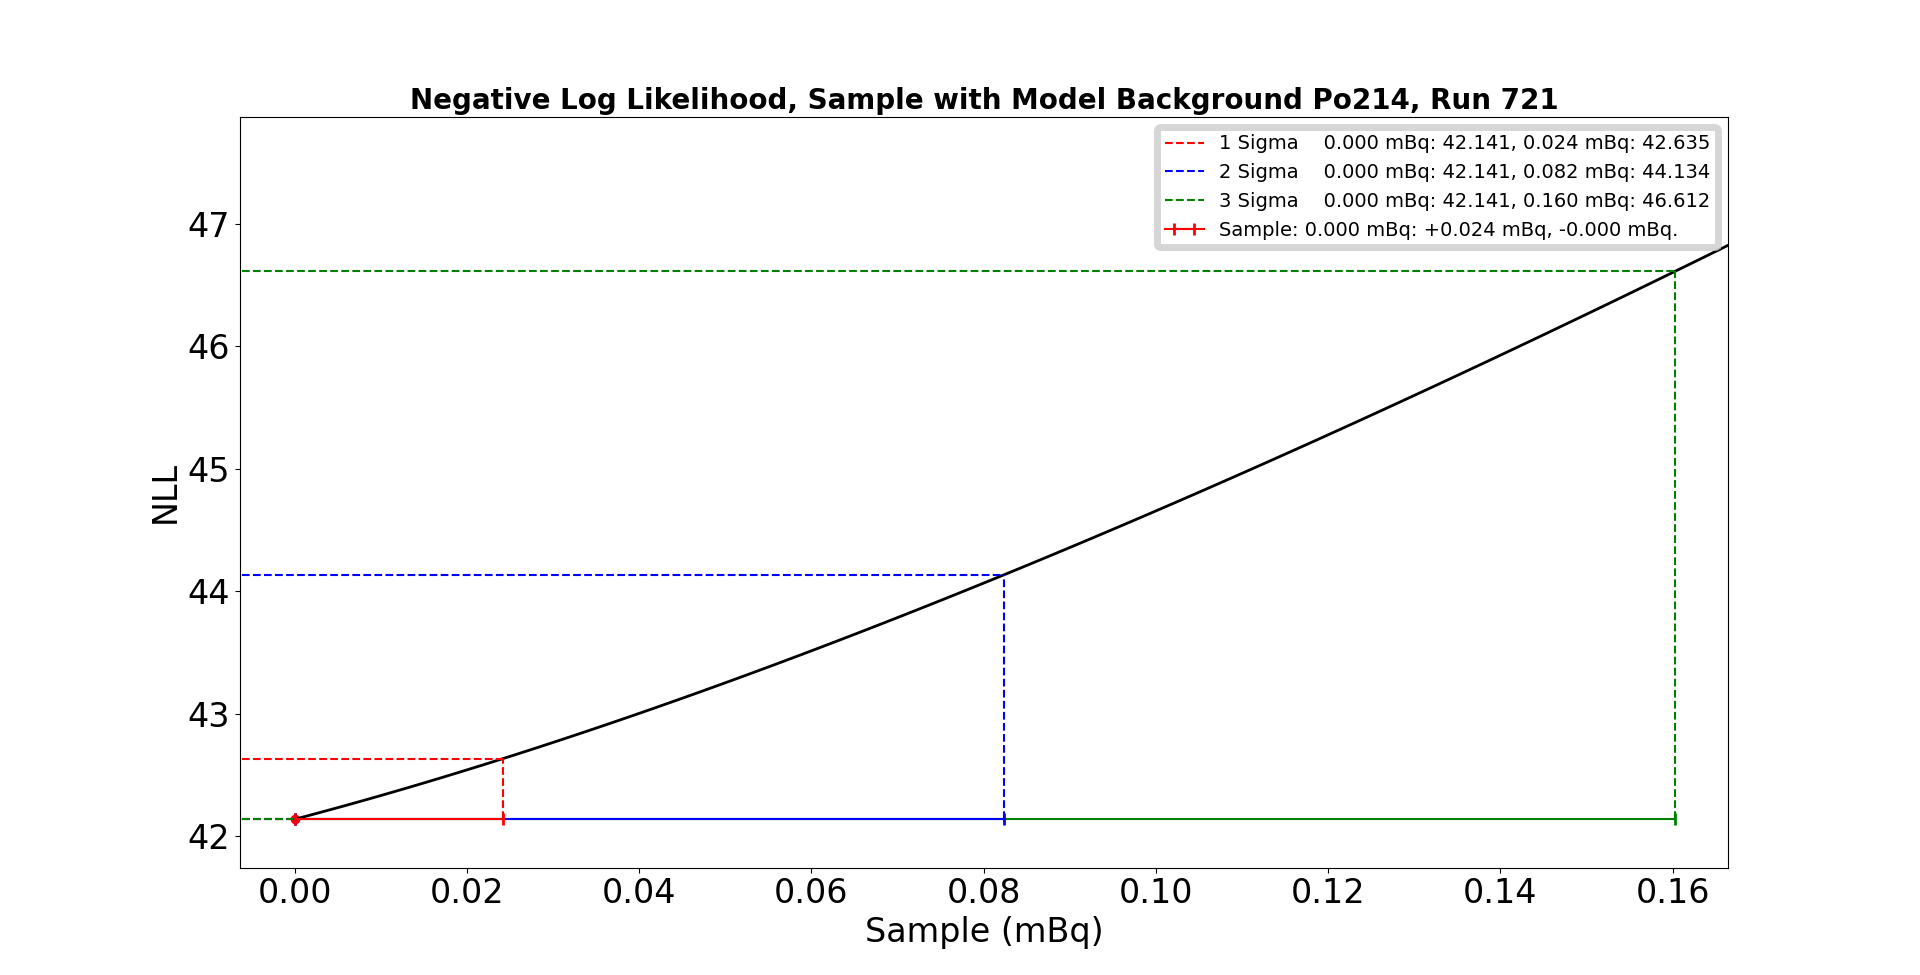
\includegraphics[width=0.9\textwidth]
            {assets/721/NLL214.png}
            \caption{This is the rate that was used to determine the emanation rate of Run 721}
        \end{center}
    \end{figure}
\end{frame}

\begin{frame}{Live Time Efficiency}
    \begin{figure}
        \begin{center}
            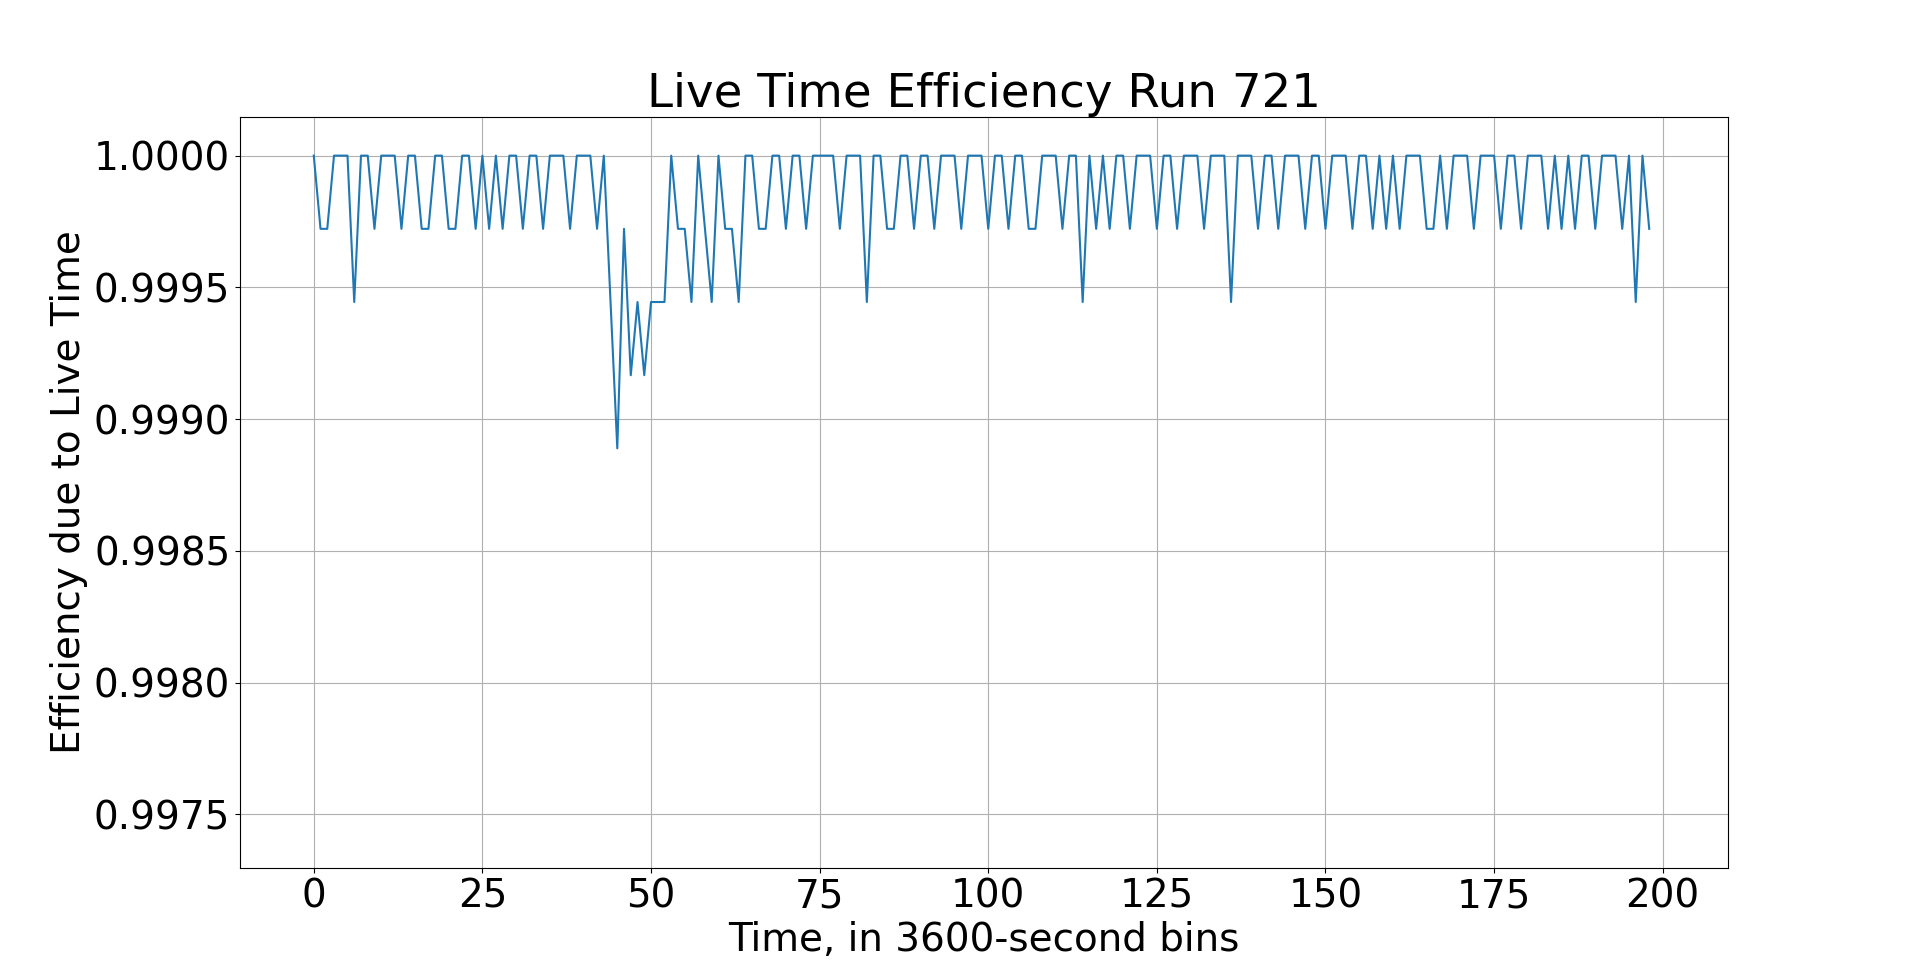
\includegraphics[width=0.9\textwidth]
            {assets/721/LTE.png}
            \caption{Detector had relatively little dead time}
        \end{center}
    \end{figure}
\end{frame}

\begin{frame}{Notes on Run 721 Analysis}
    Run 721 exhibits low gain that appears to vary periodically.
    Unfortunately, there is no environmental data to compare the shifts to.
    Several bins had to be cut due to high noise.
    The low resolution exhibited by Run 721 gives way to $^{210}$Po events spilling over
    into the $^{218}$Po ROI.
    Because of this, the $^{214}$Po rate alone was used to determine the emanation rate
    for run 721.
    Overall, Run 721 appears to be consistent with our backgrounds.

    \hyperlink{RvT_721}{\beamerbutton{Back to Rate vs Time Run 721}}
\end{frame}

\begin{frame}{Run 722 Backup Slides}
\label{722_Backup}
    The following slides contain additional data and information regarding Run 722.
\end{frame}

\begin{frame}{Raw Data, Run 722}
    \begin{figure}
        \begin{center}
            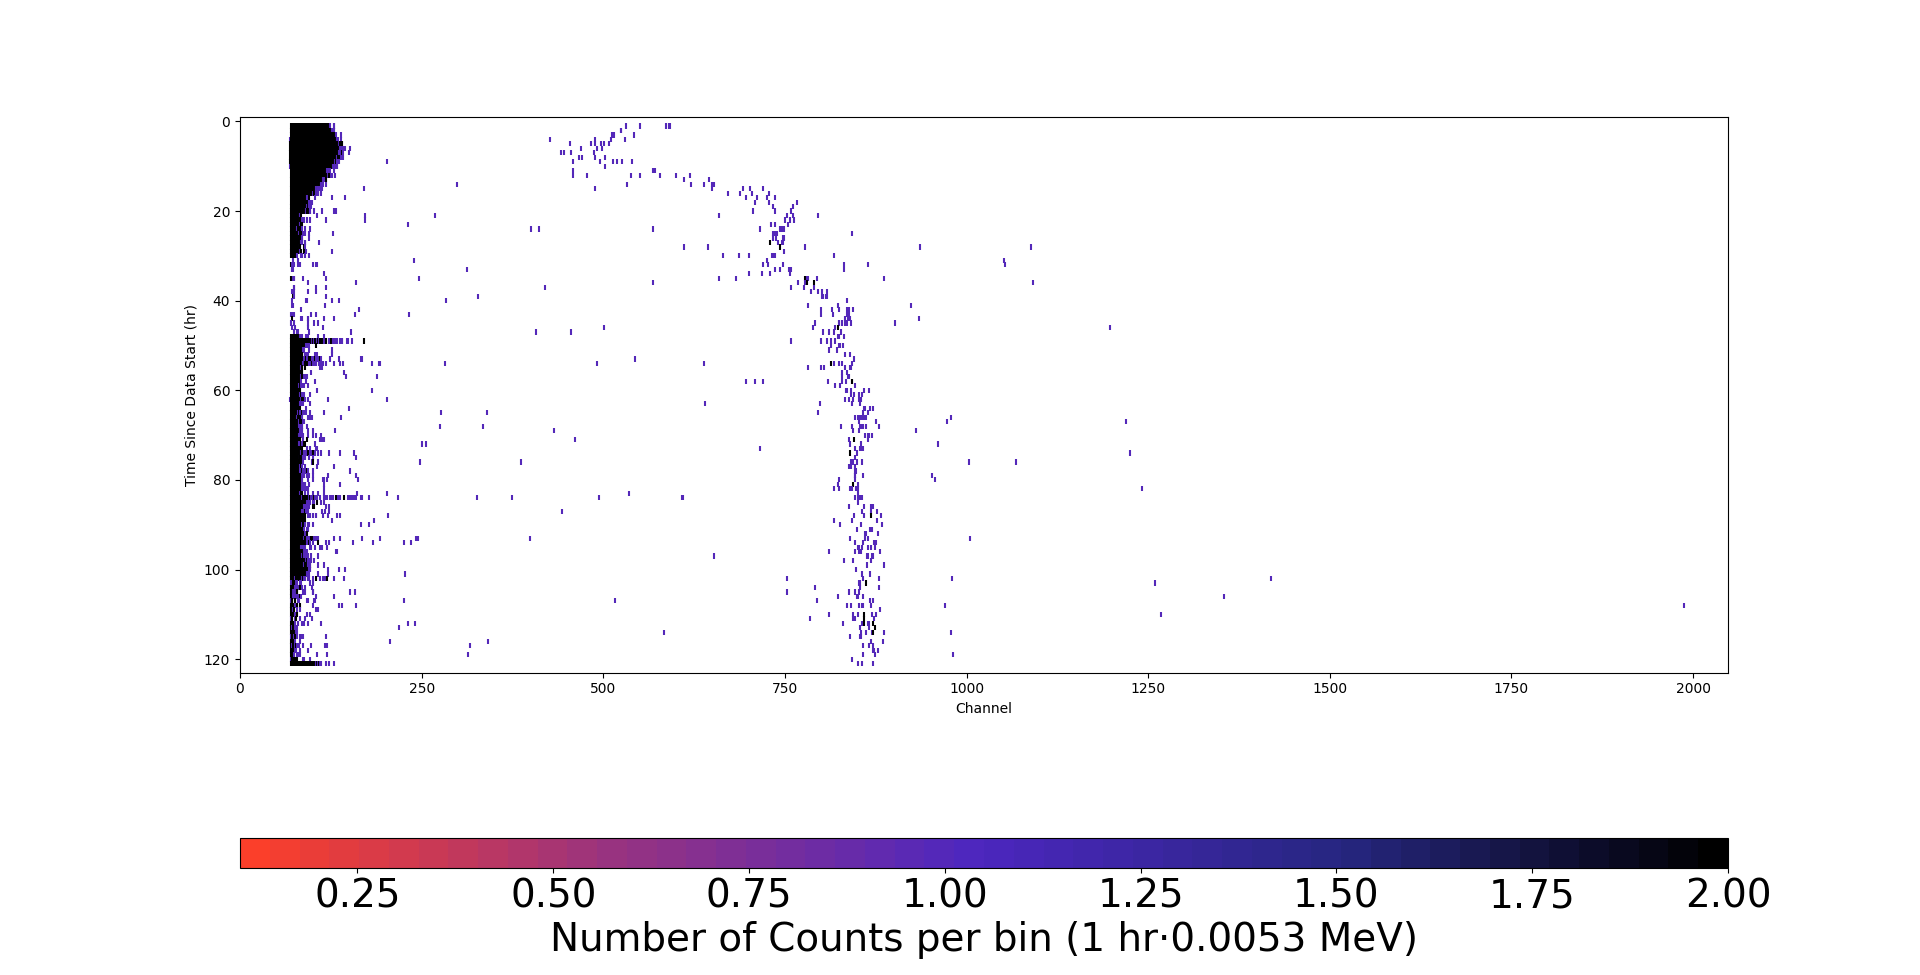
\includegraphics[width=0.9\textwidth]
            {assets/722/RD.png}
            \caption{Run 722 exhibited such extreme gain shift that hours had to be removed to enable gain correction}
        \end{center}
    \end{figure}
\end{frame}

\begin{frame}{Raw Data after Removing Bad Intervals, Run 722}
    \begin{figure}
        \begin{center}
            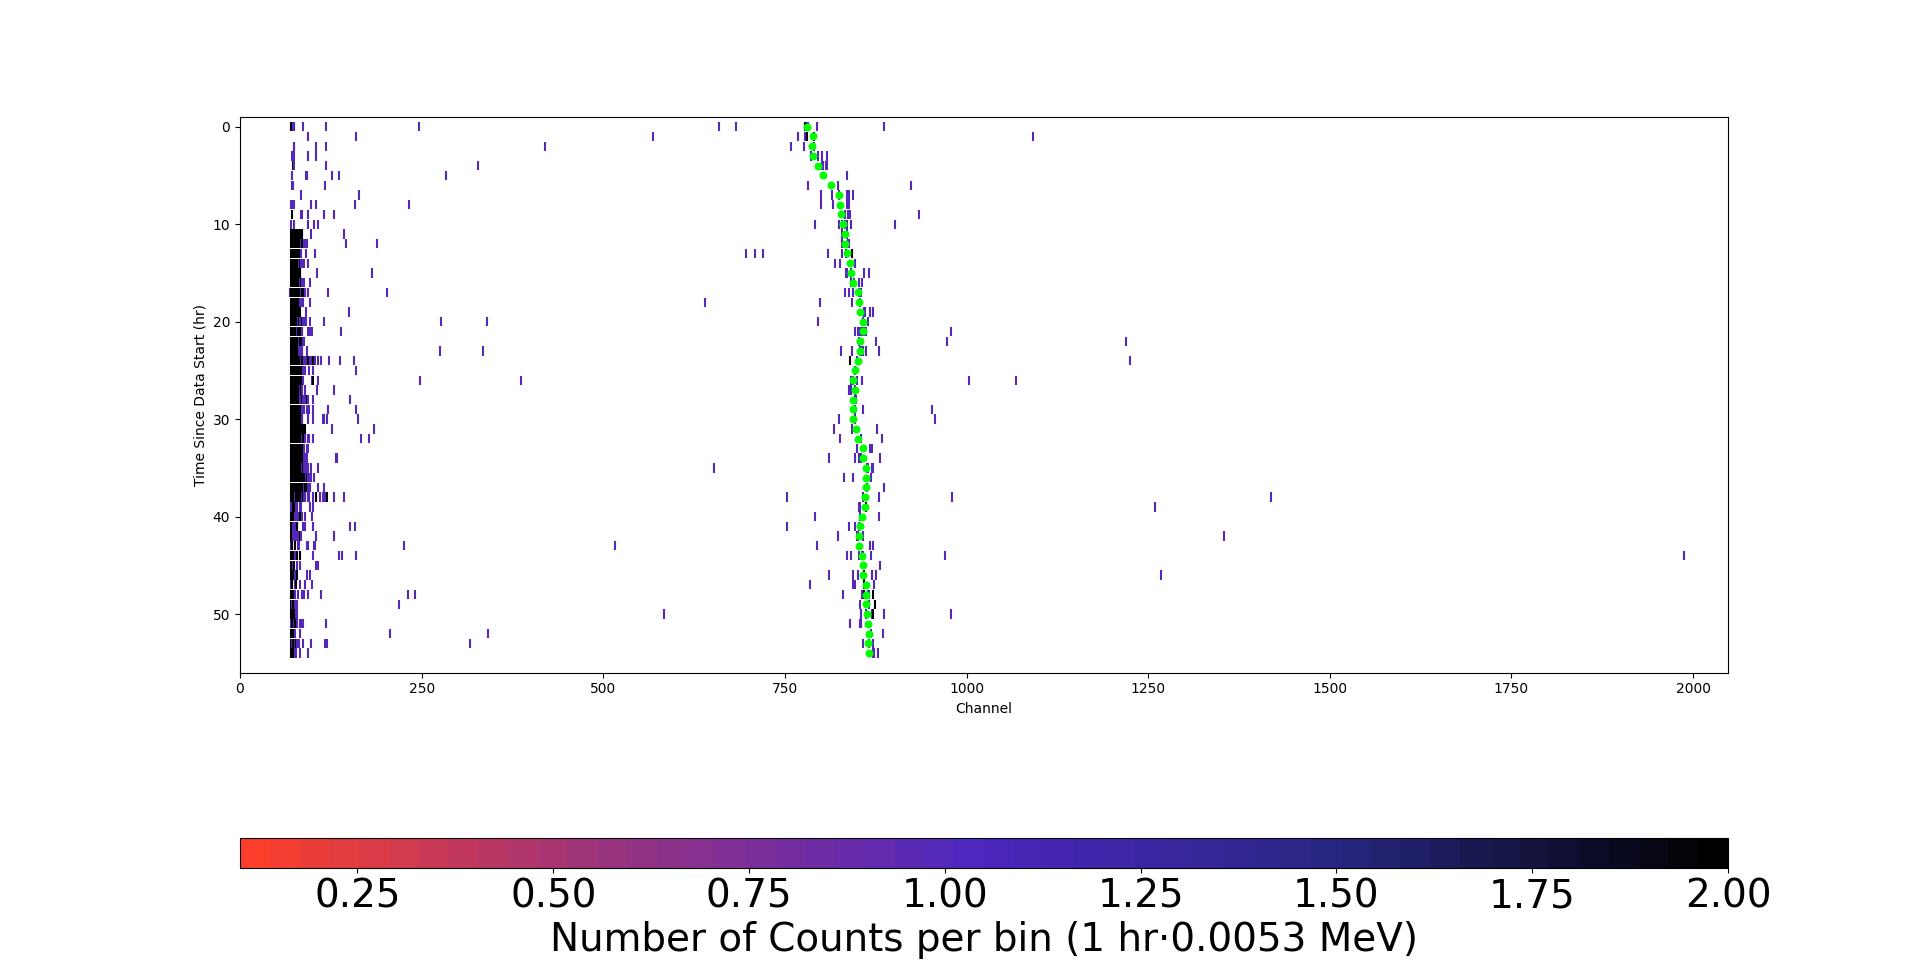
\includegraphics[width=0.9\textwidth]
            {assets/722/RDP.png}
            \caption{Data exhibits less extreme gain shifts and is able to be gain corrected}
        \end{center}
    \end{figure}
\end{frame}

\begin{frame}{Gain-Corrected Data, Run 722}
    \begin{figure}
        \begin{center}
            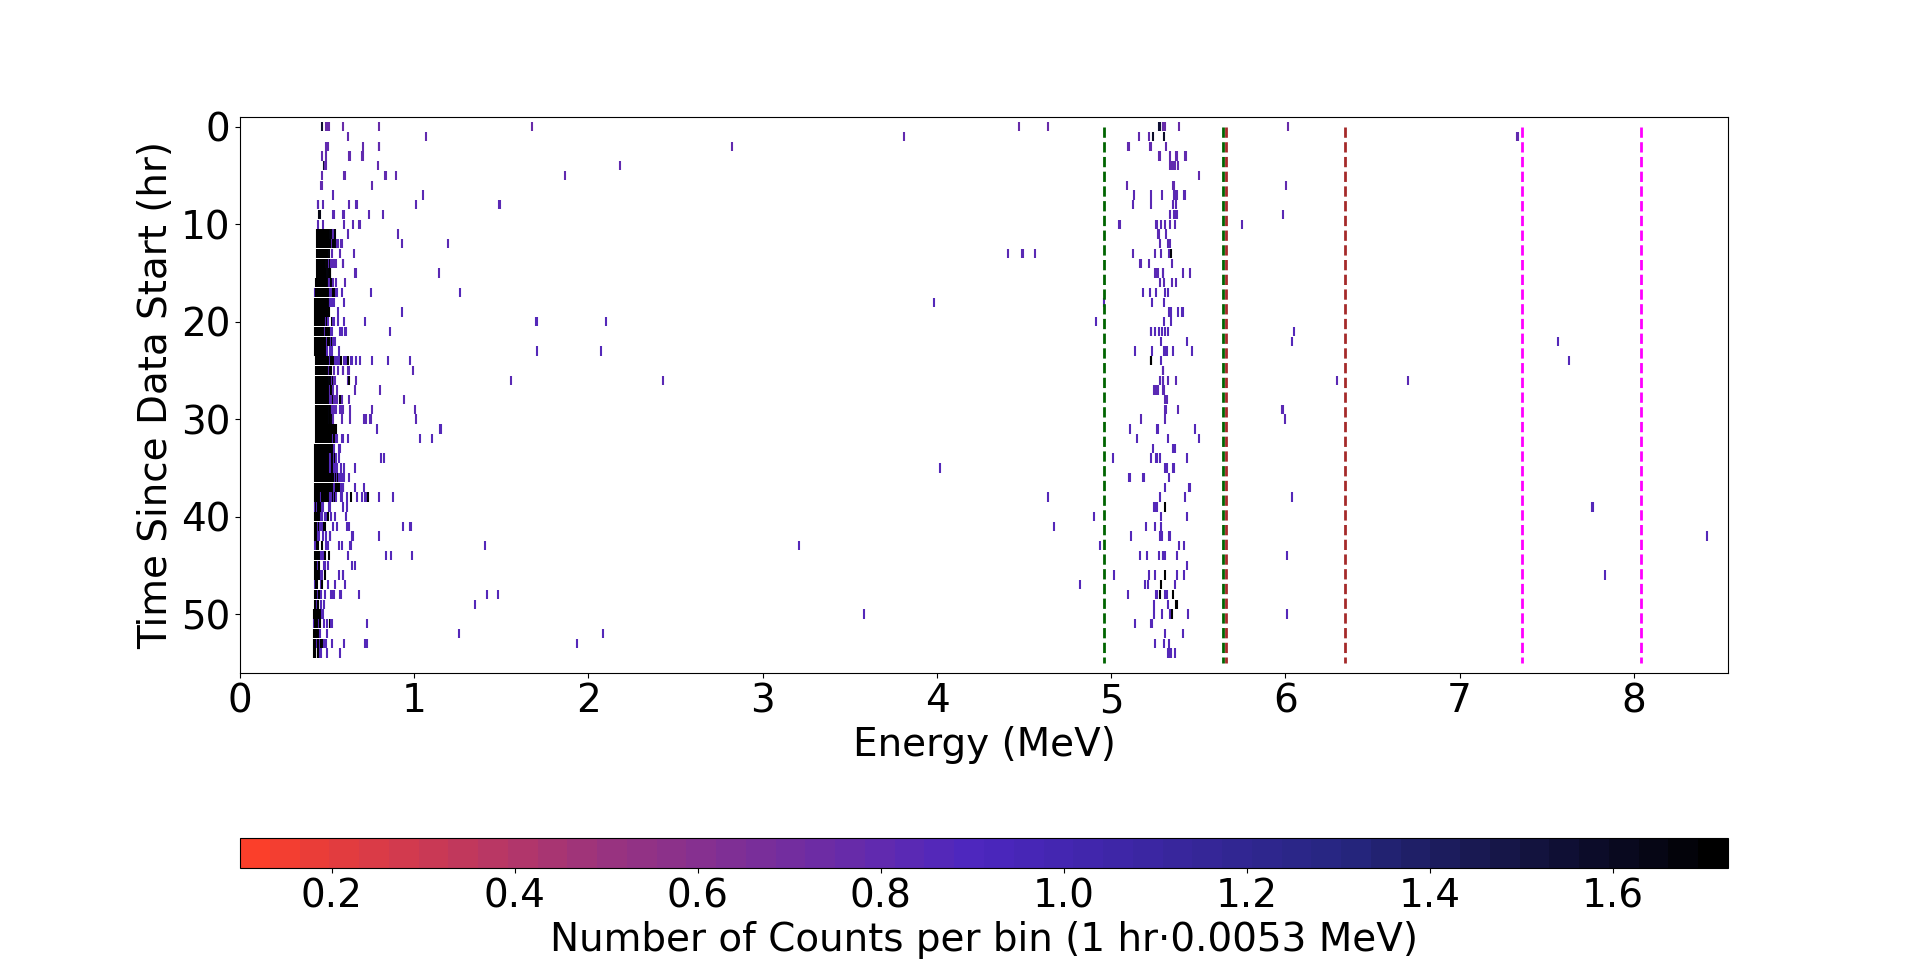
\includegraphics[width=0.9\textwidth]
            {assets/722/CD.png}
            \caption{Data exibits relatively good resolution and no spillage is apparent}
        \end{center}
    \end{figure}
\end{frame}

\begin{frame}{Counts vs. Energy, Run 722}
    \begin{figure}
        \begin{center}
            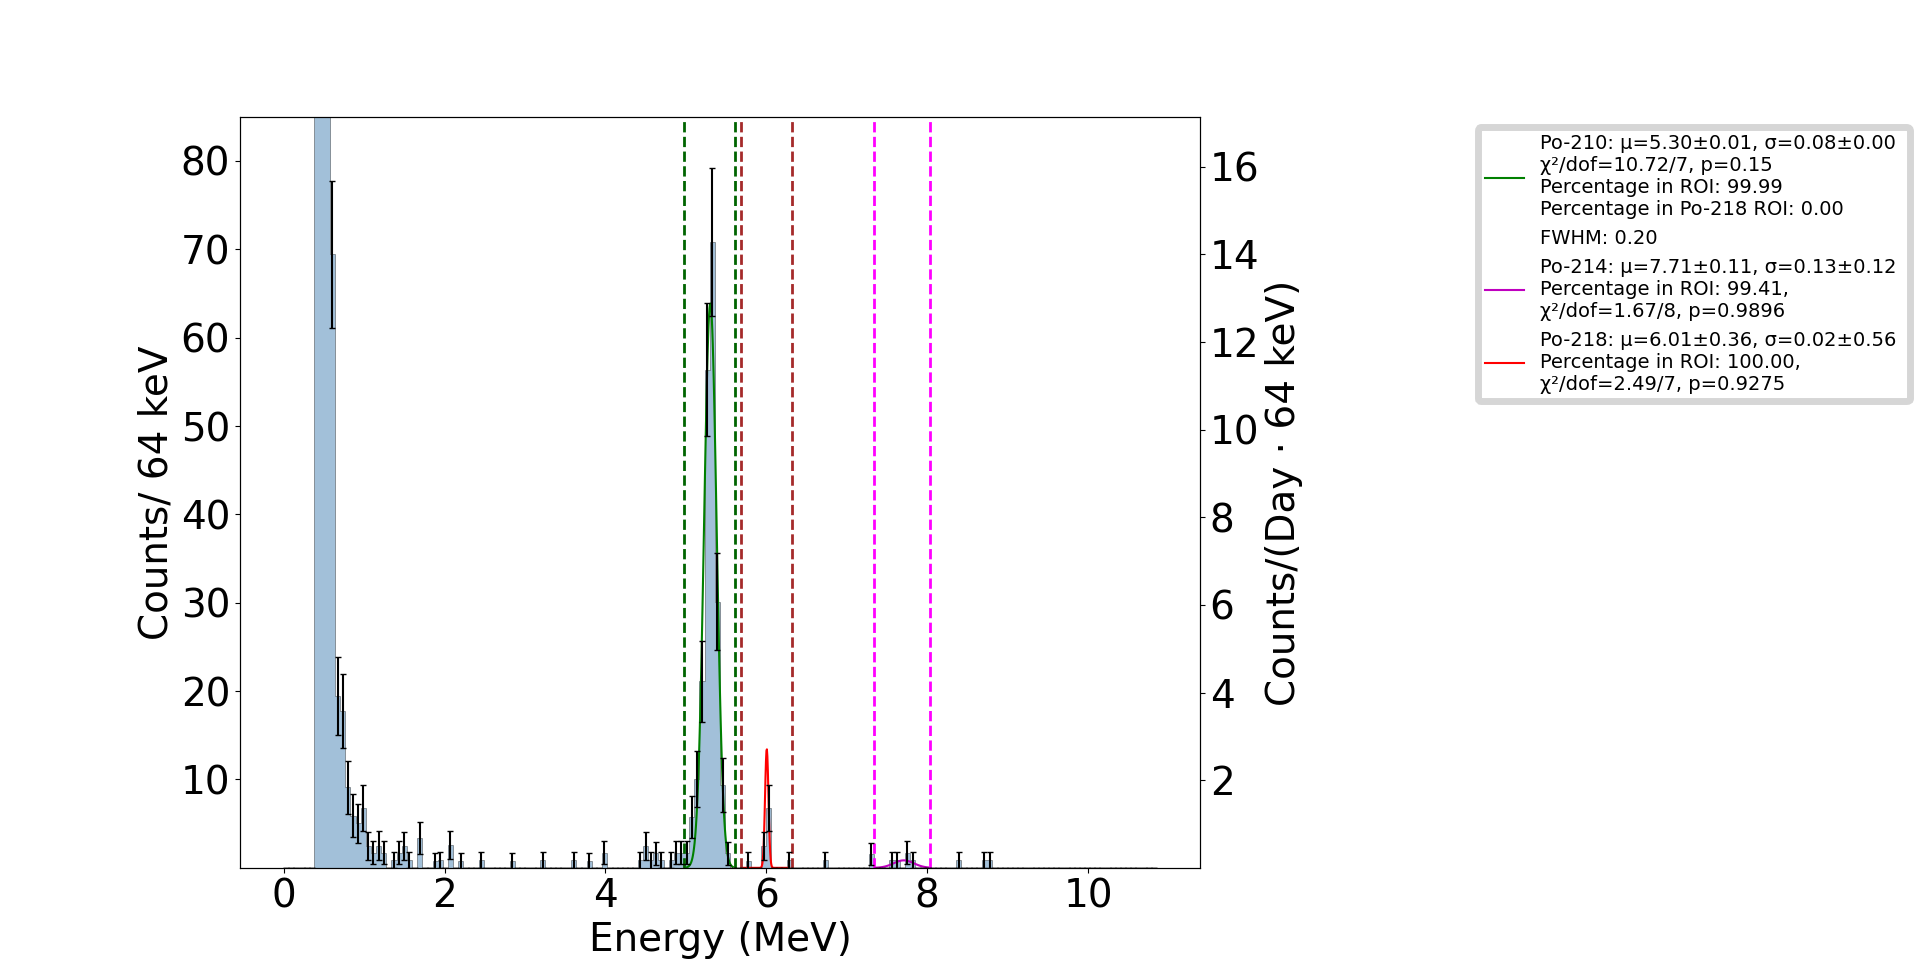
\includegraphics[width=0.9\textwidth]
            {assets/722/CvE.png}
            \caption{Each peak exhibits good resolution}
        \end{center}
    \end{figure}
\end{frame}

\begin{frame}{Combined NLL, Run 722}
    \begin{figure}
        \begin{center}
            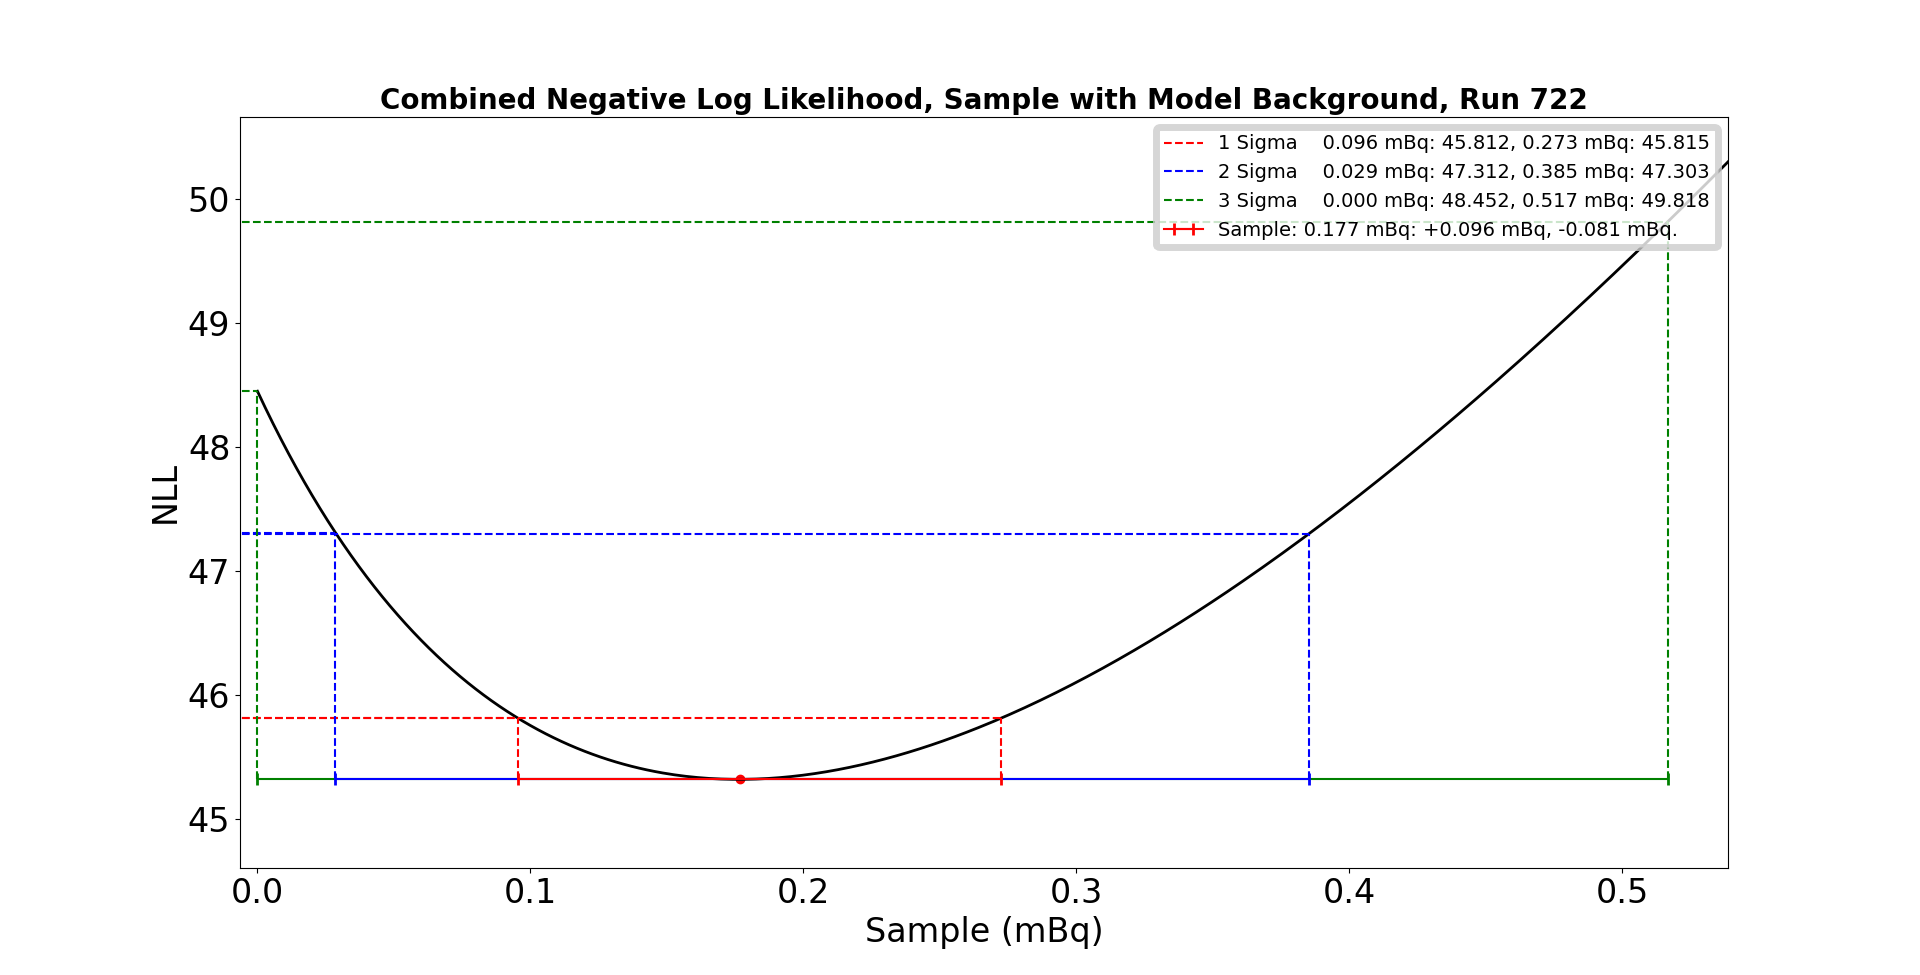
\includegraphics[width=0.9\textwidth]
            {assets/722/comNLL.png}
            \caption{This rate is used for the emanation rate for Run 722}
        \end{center}
    \end{figure}
\end{frame}

\begin{frame}{$^{218}$Po NLL, Run 722}
    \begin{figure}
        \begin{center}
            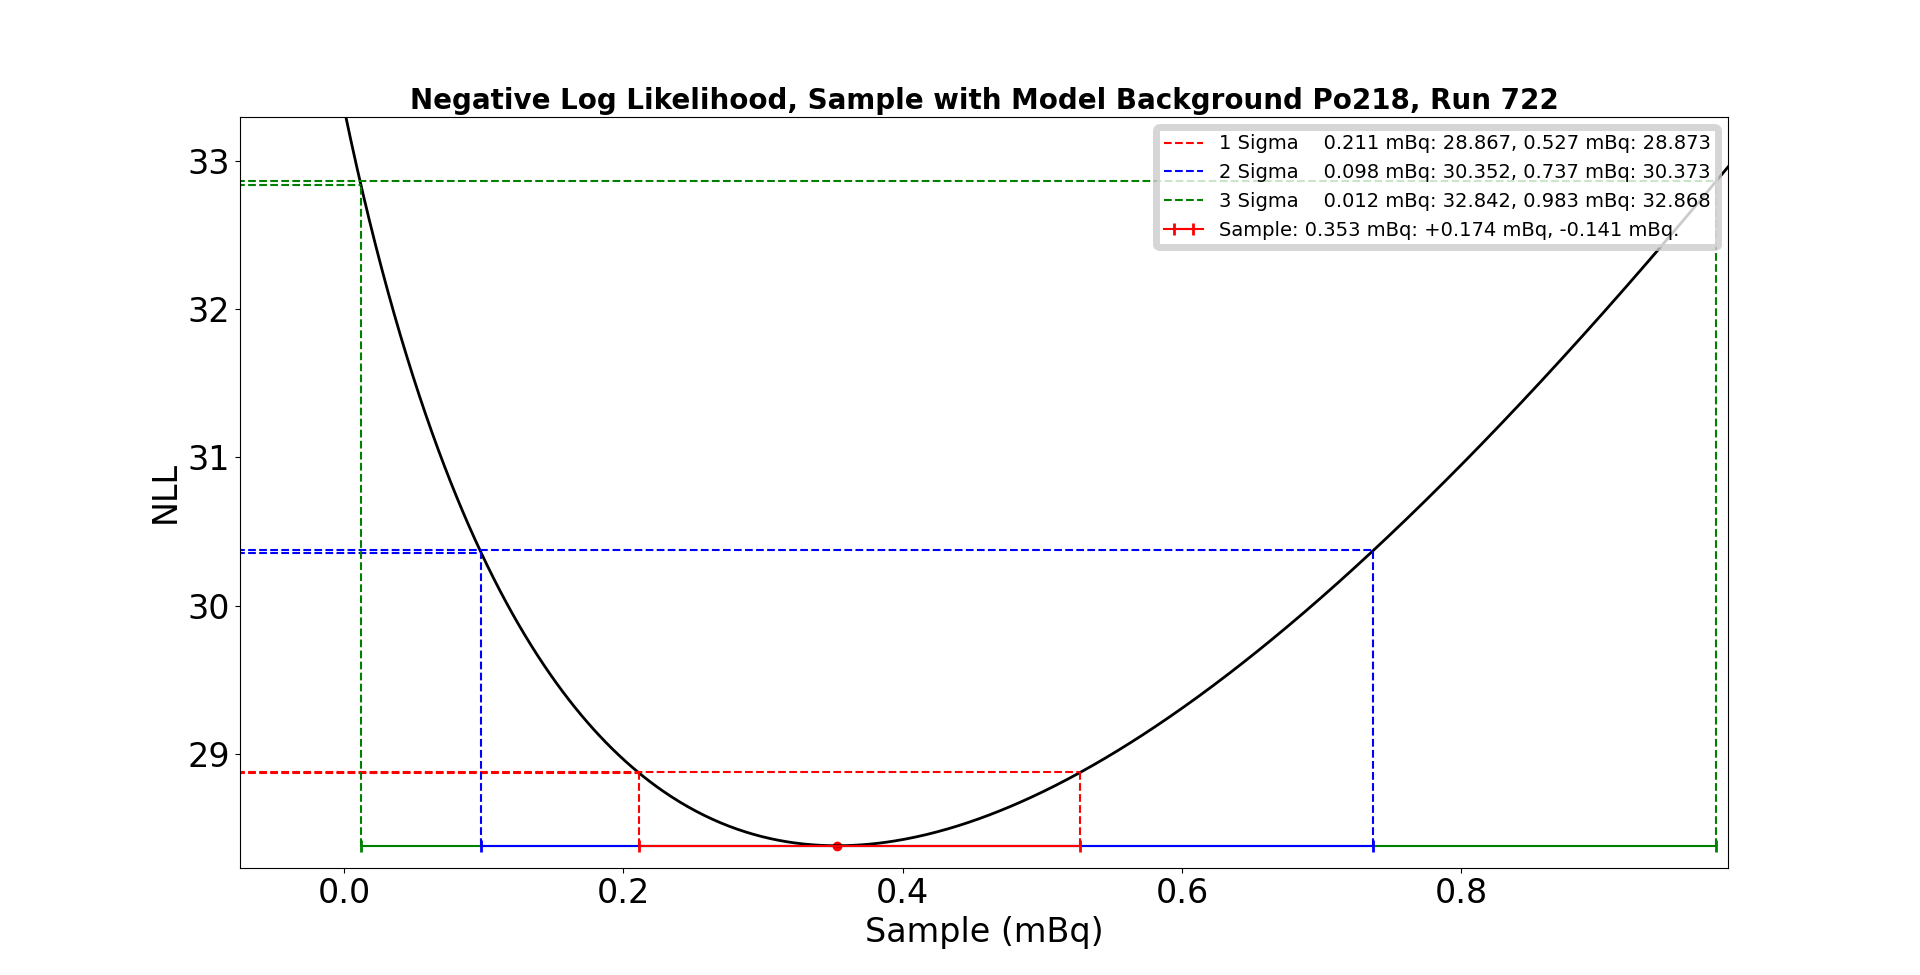
\includegraphics[width=0.9\textwidth]
            {assets/722/NLL218.png}
            \caption{This rate is used to determine the combined rate}
        \end{center}
    \end{figure}
\end{frame}

\begin{frame}{$^{214}$Po NLL, Run 722}
    \begin{figure}
        \begin{center}
            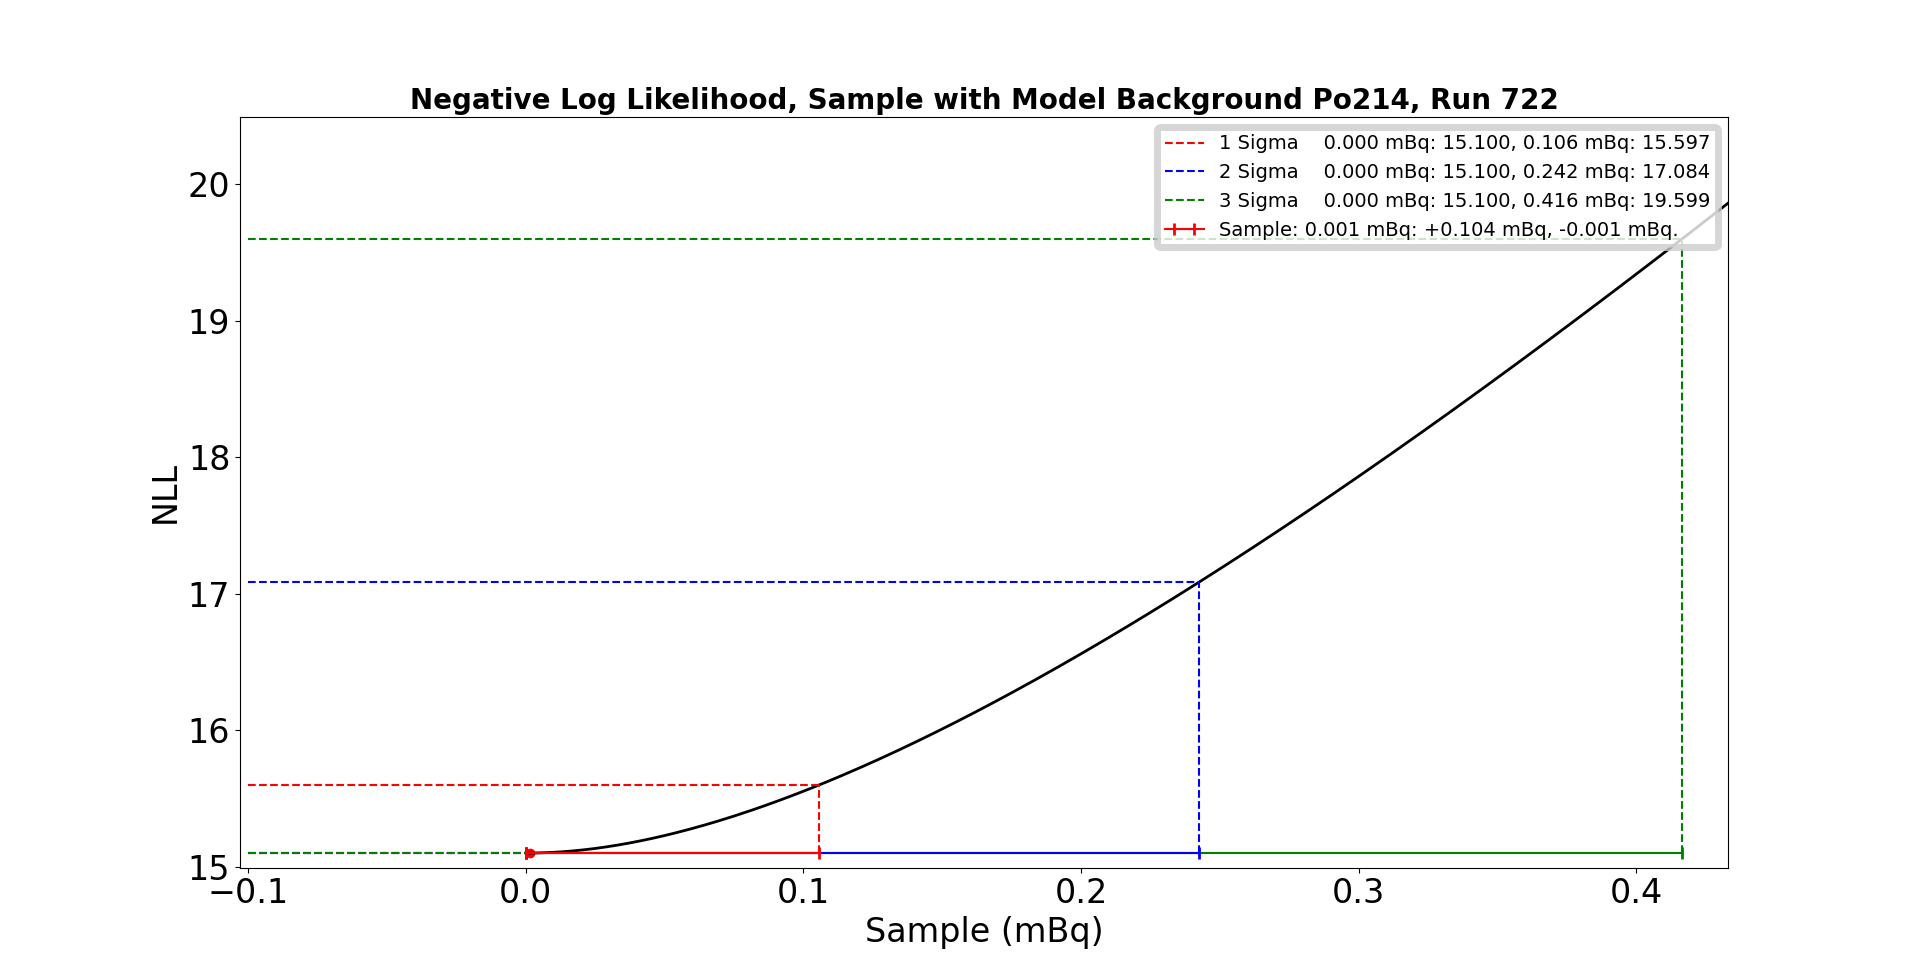
\includegraphics[width=0.9\textwidth]
            {assets/722/NLL214.png}
            \caption{This rate is used to determine the combined rate}
        \end{center}
    \end{figure}
\end{frame}

\begin{frame}{Live Time Efficiency}
    \begin{figure}
        \begin{center}
            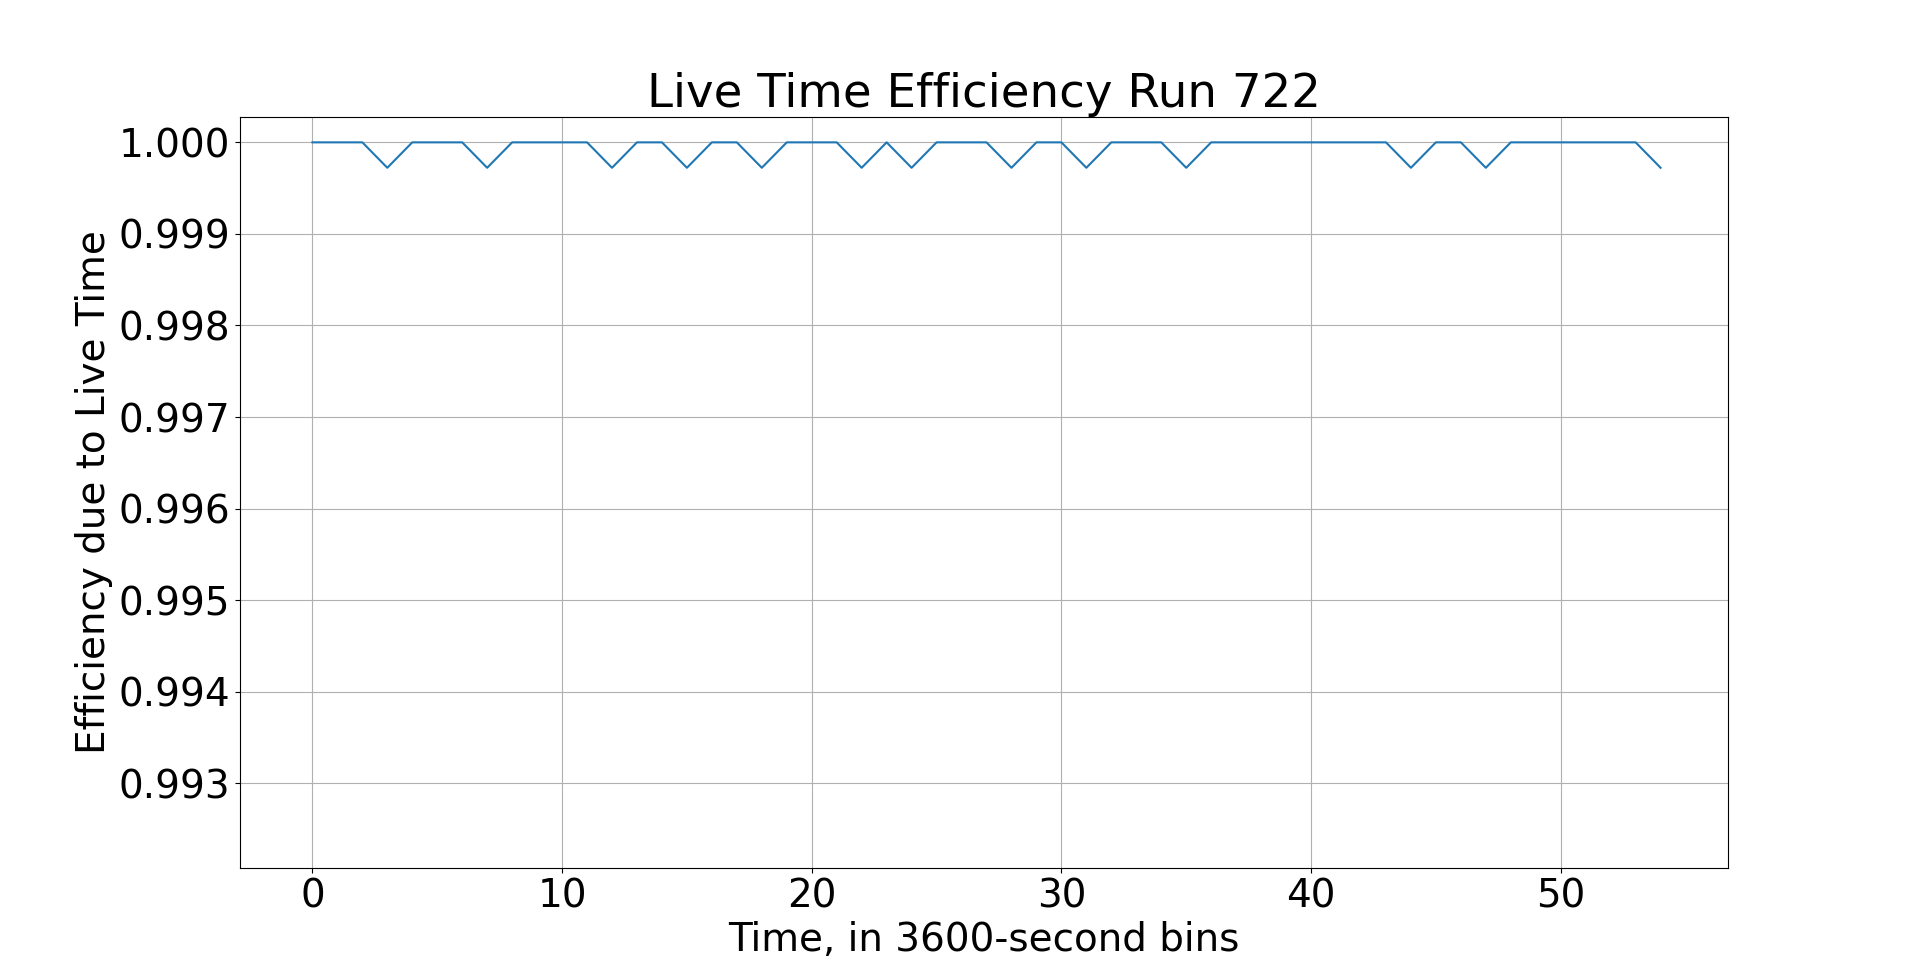
\includegraphics[width=0.9\textwidth]
            {assets/722/LTE.png}
            \caption{Detector had relatively little dead time}
        \end{center}
    \end{figure}
\end{frame}

\begin{frame}{Notes on Run 722 Analysis}
    Run 722 exhibits such extreme shifts in gain that peak finding was impossible without removing 
    several hours of data.
    However, there is better resolution and the combined rate was able to be utilized for this run.


    \hyperlink{RvT_722}{\beamerbutton{Back to Rate vs Time Run 722}}
\end{frame}

\begin{frame}{Run 730 Backup Slides}
\label{730_Backup}
    The following slides contain additional data and information regarding Run 730.
\end{frame}

\begin{frame}{Raw Data, Run 730}
    \begin{figure}
        \begin{center}
            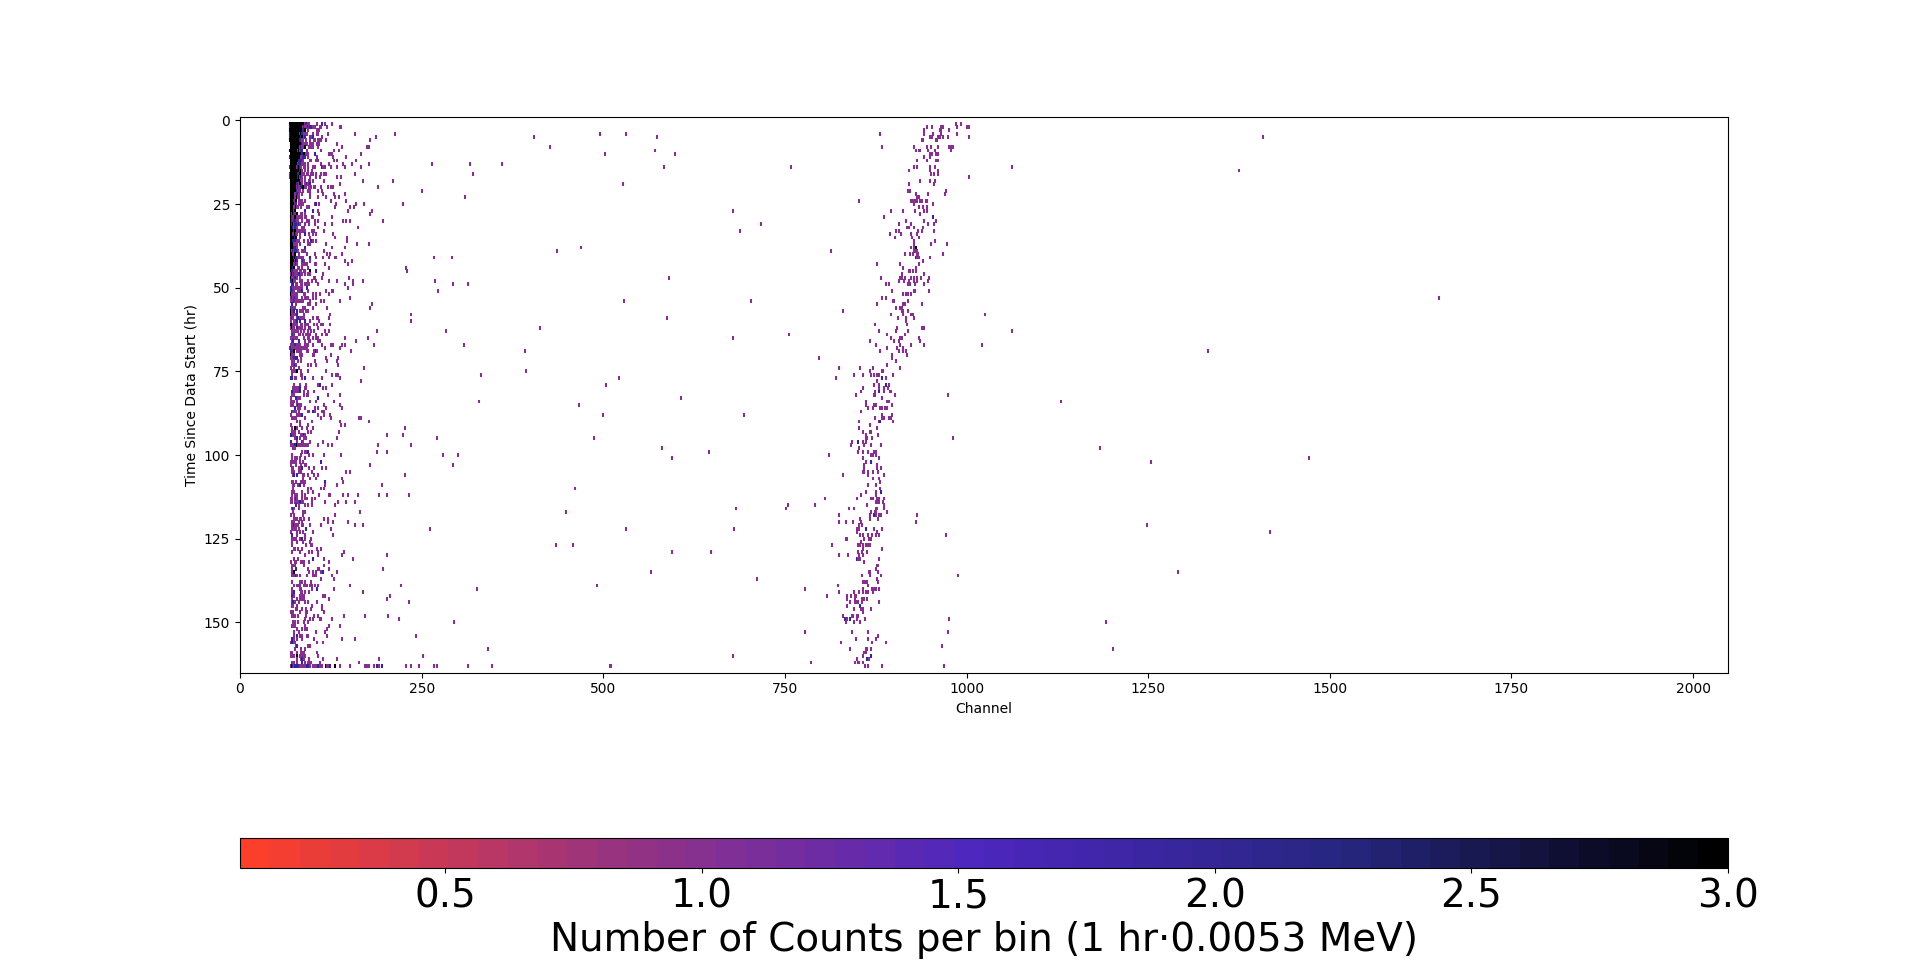
\includegraphics[width=0.9\textwidth]
            {assets/730/RD.png}
            \caption{Run 730 exhibited such extreme gain shift that hours had to be removed to enable gain correction}
        \end{center}
    \end{figure}
\end{frame}

\begin{frame}{Raw Data after Removing Bad Intervals, Run 730}
    \begin{figure}
        \begin{center}
            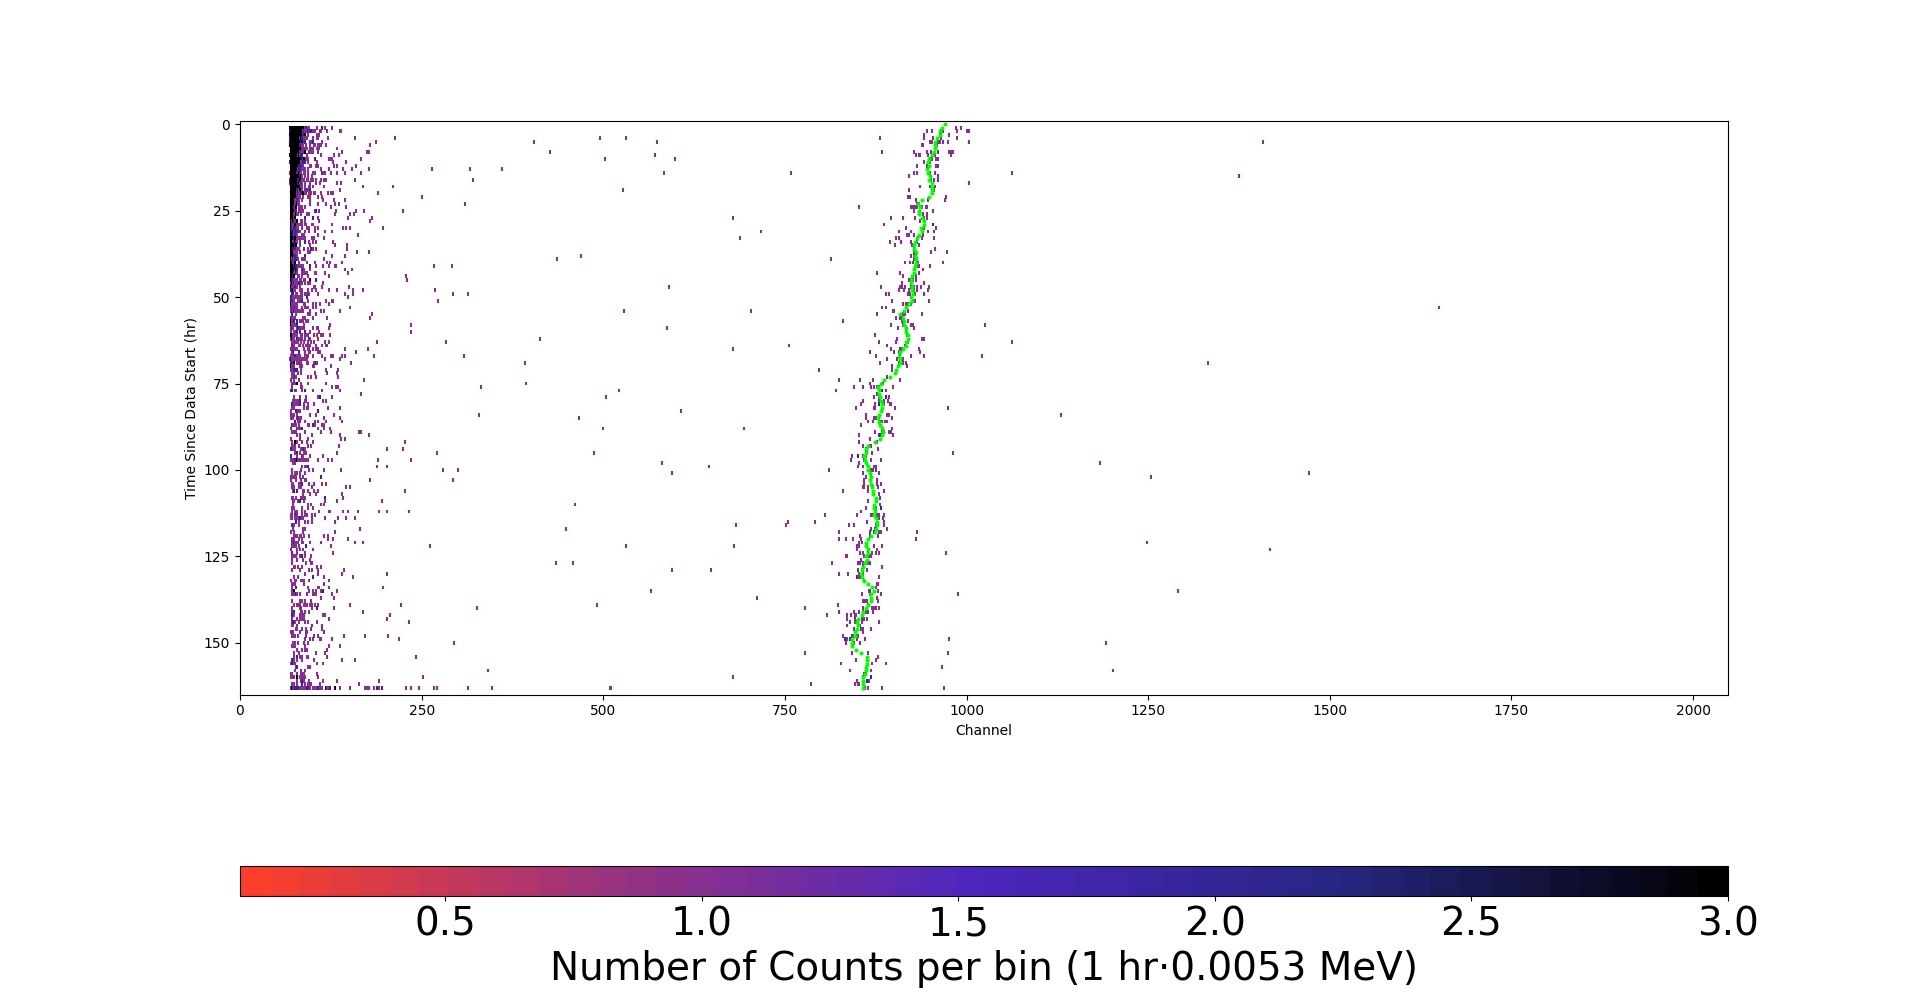
\includegraphics[width=0.9\textwidth]
            {assets/730/RDP.png}
            \caption{Data exhibits less extreme gain shifts and is able to be gain corrected}
        \end{center}
    \end{figure}
\end{frame}

\begin{frame}{Gain-Corrected Data, Run 730}
    \begin{figure}
        \begin{center}
            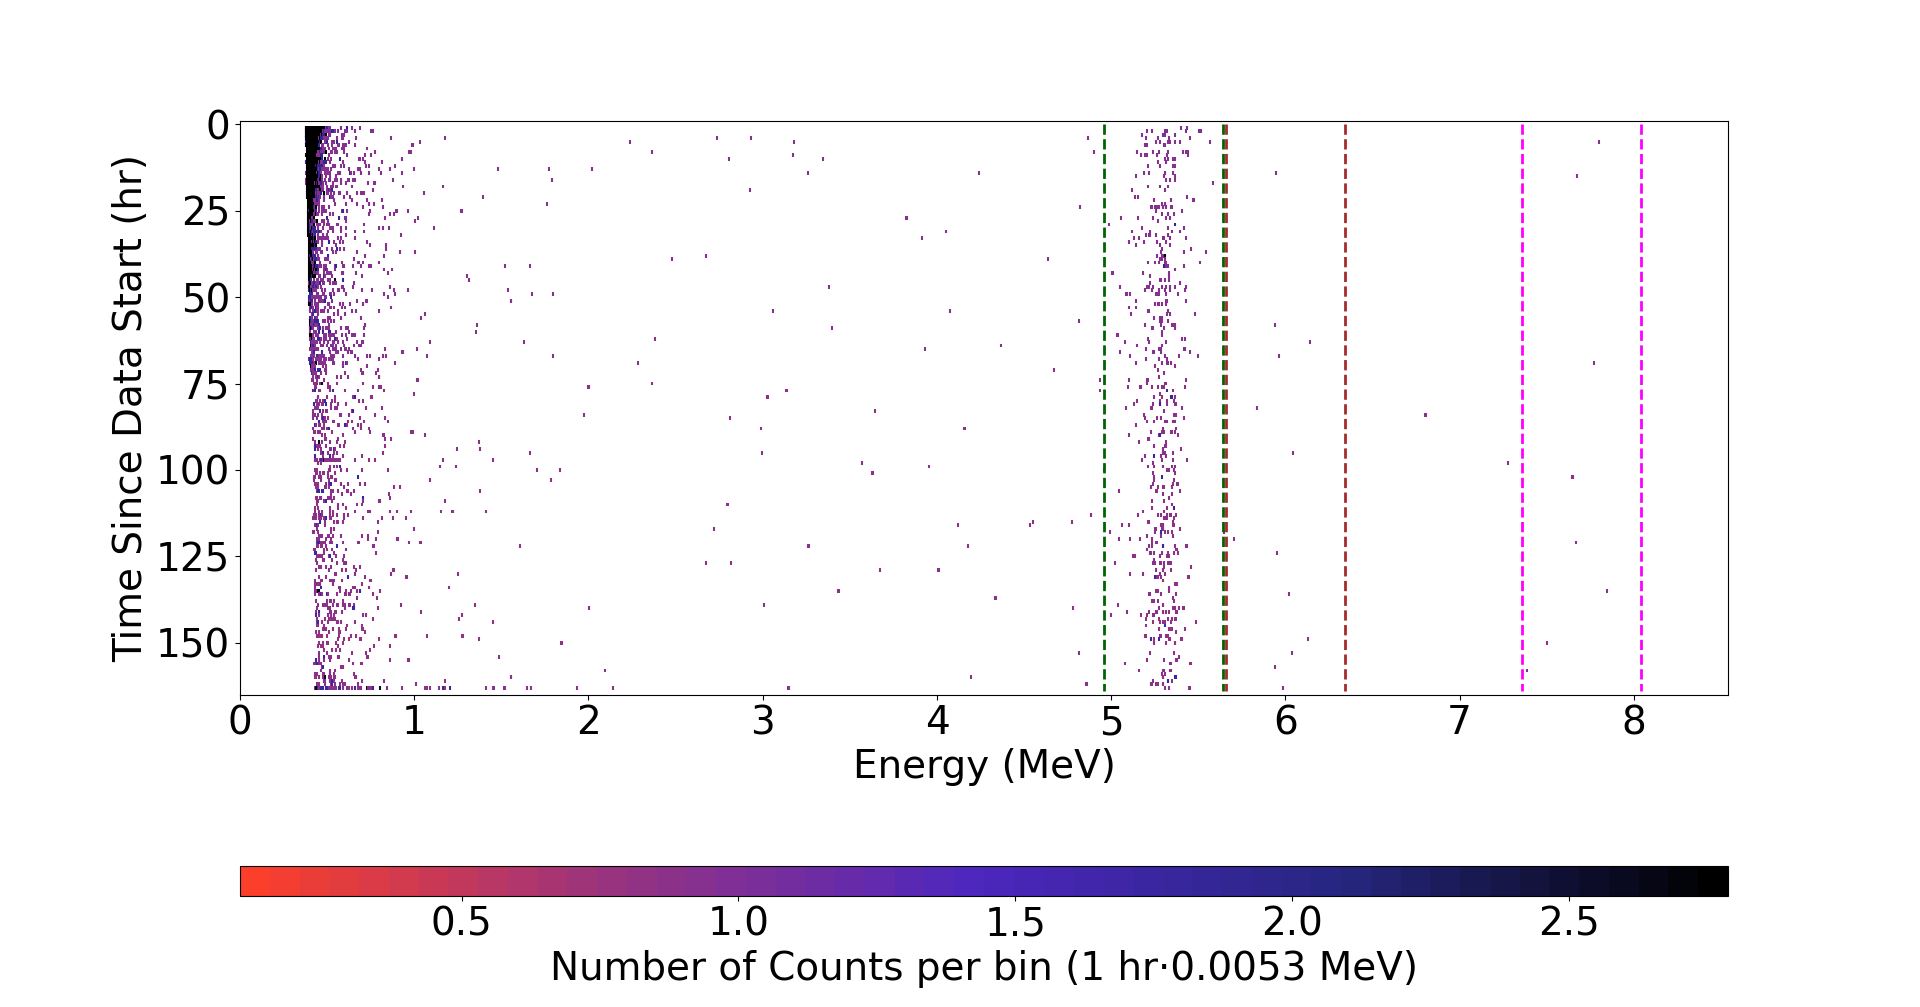
\includegraphics[width=0.9\textwidth]
            {assets/730/CD.png}
            \caption{Data exibits relatively good resolution and no spillage is apparent}
        \end{center}
    \end{figure}
\end{frame}

\begin{frame}{Counts vs. Energy, Run 730}
    \begin{figure}
        \begin{center}
            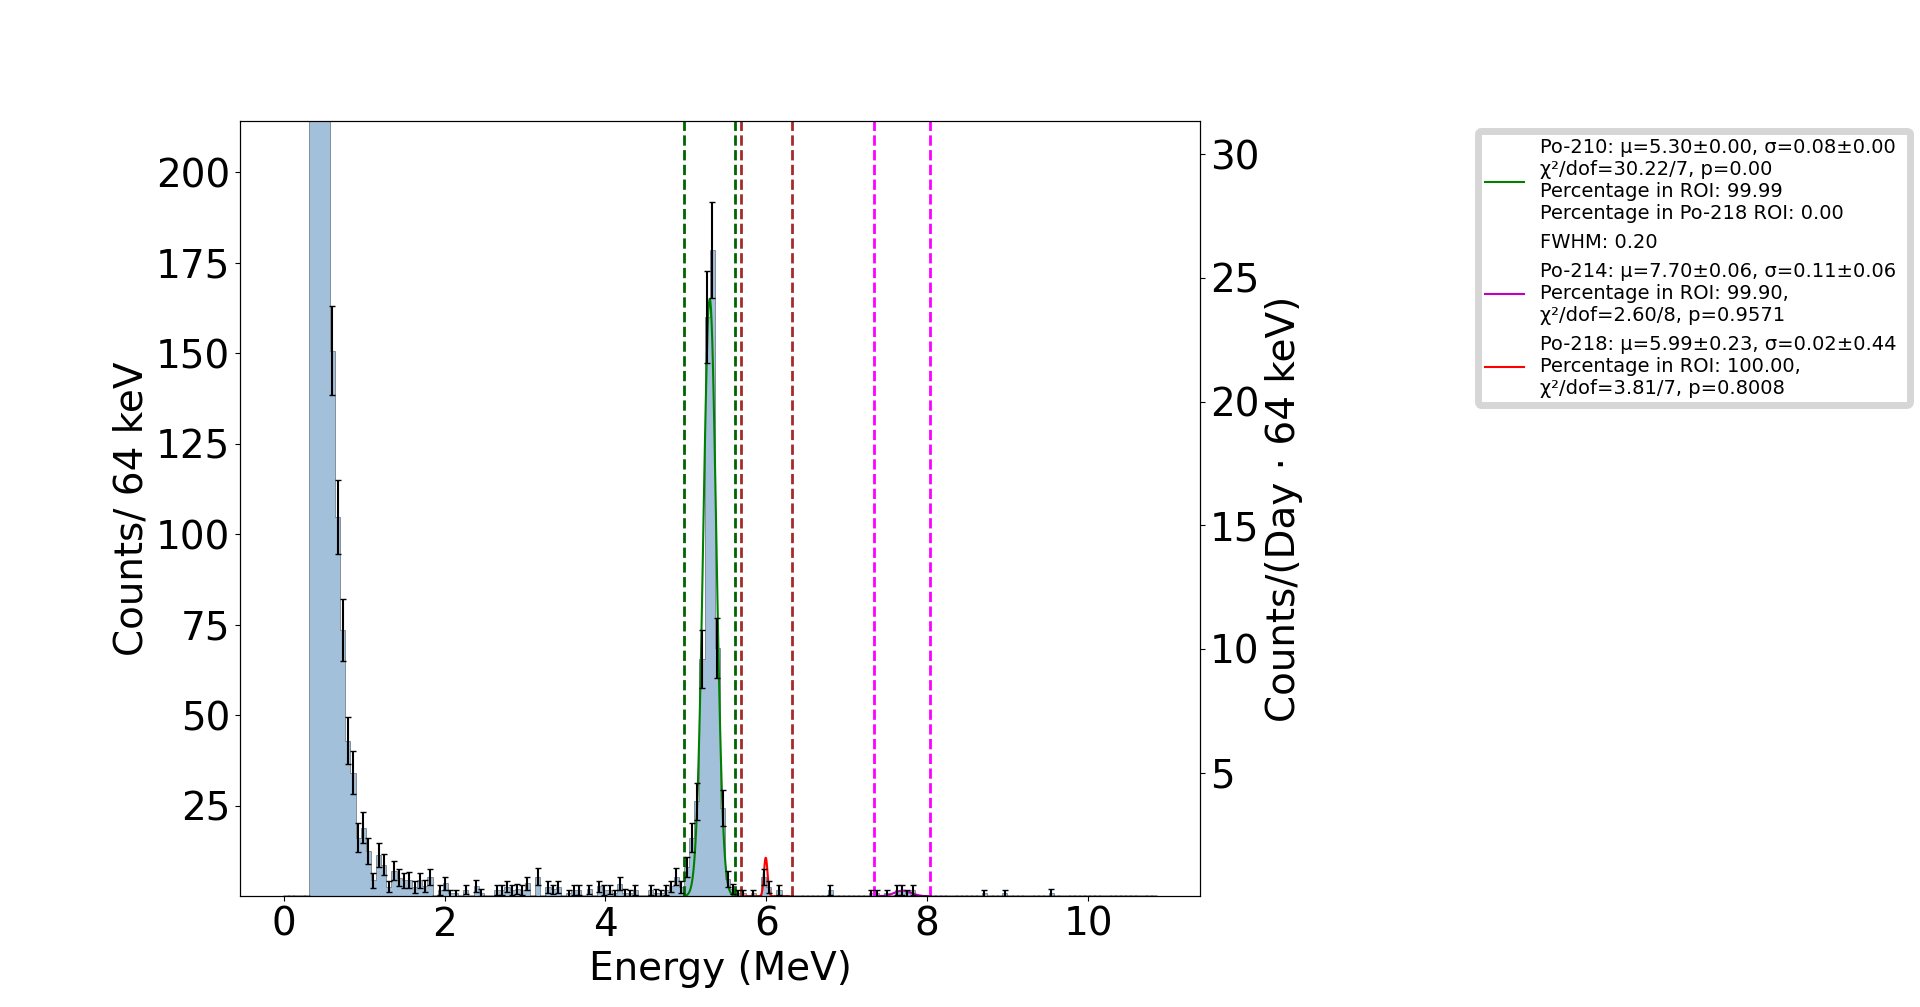
\includegraphics[width=0.9\textwidth]
            {assets/730/CvE.png}
            \caption{Each peak exhibits good resolution}
        \end{center}
    \end{figure}
\end{frame}

\begin{frame}{Combined NLL, Run 730}
    \begin{figure}
        \begin{center}
            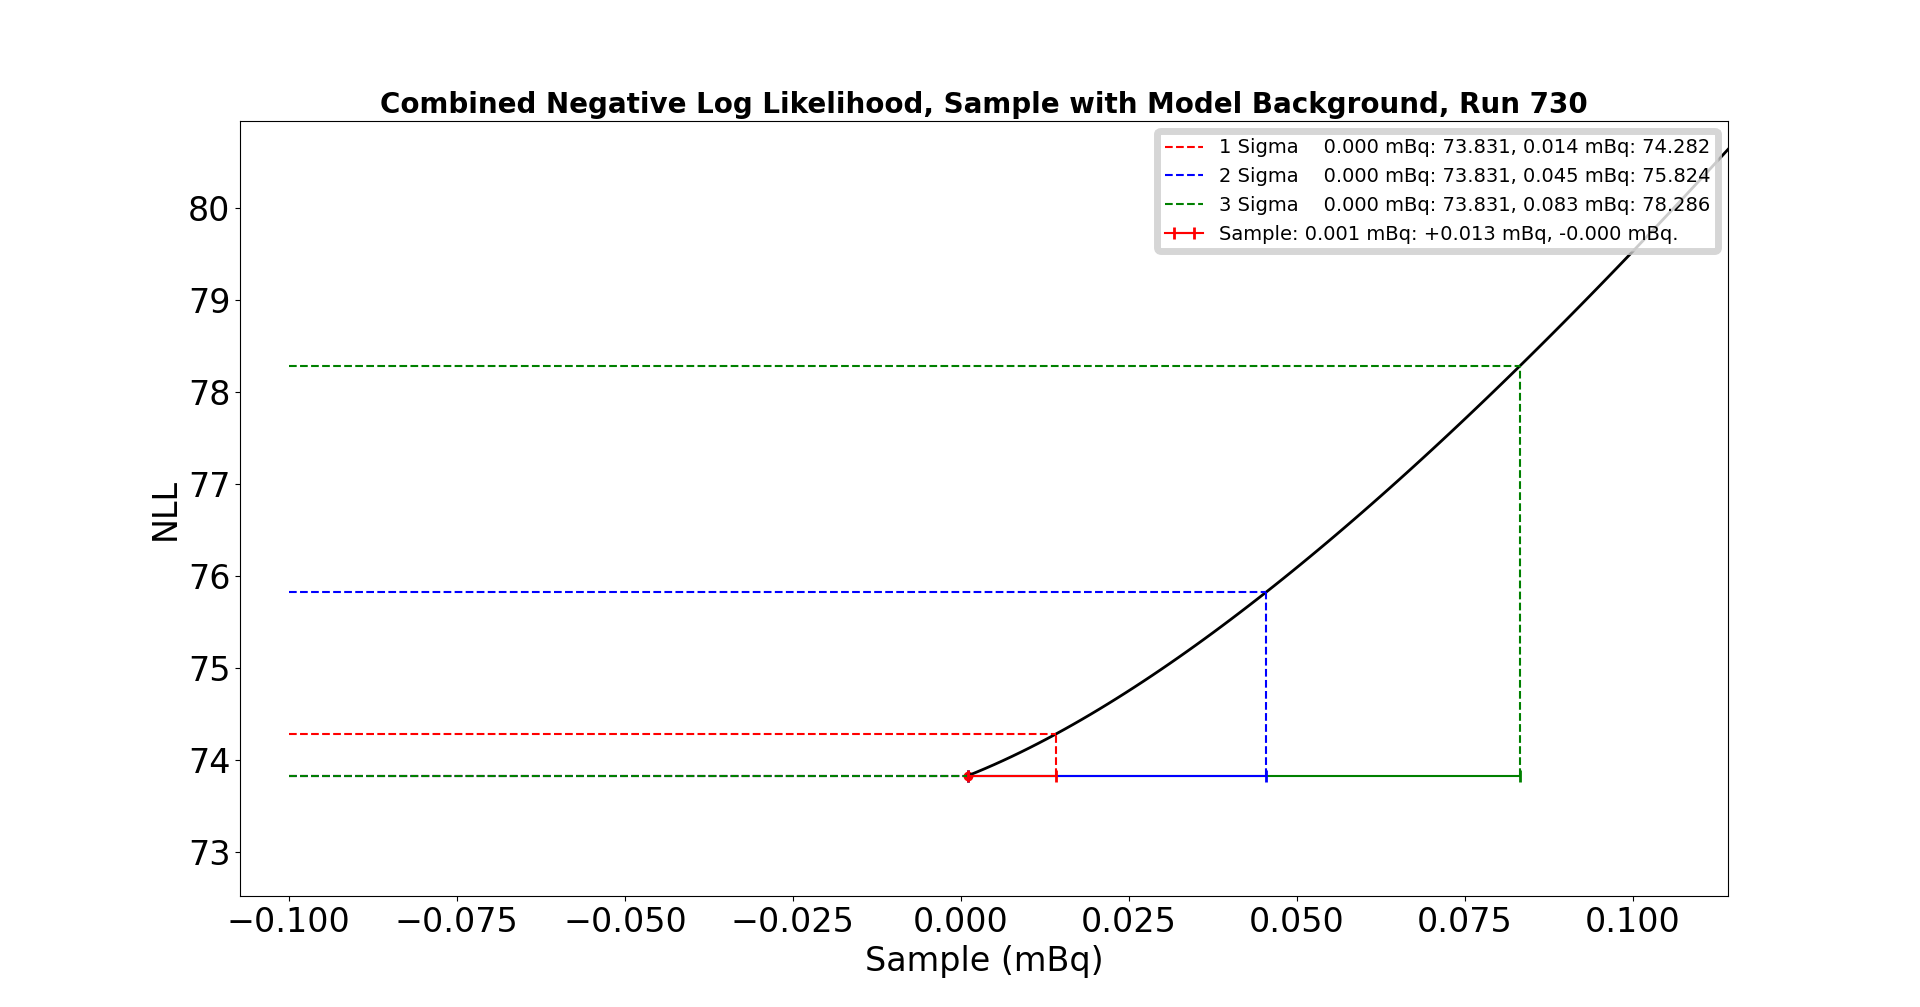
\includegraphics[width=0.9\textwidth]
            {assets/730/comNLL.png}
            \caption{This rate is used for the emanation rate for Run 730}
        \end{center}
    \end{figure}
\end{frame}

\begin{frame}{$^{218}$Po NLL, Run 730}
    \begin{figure}
        \begin{center}
            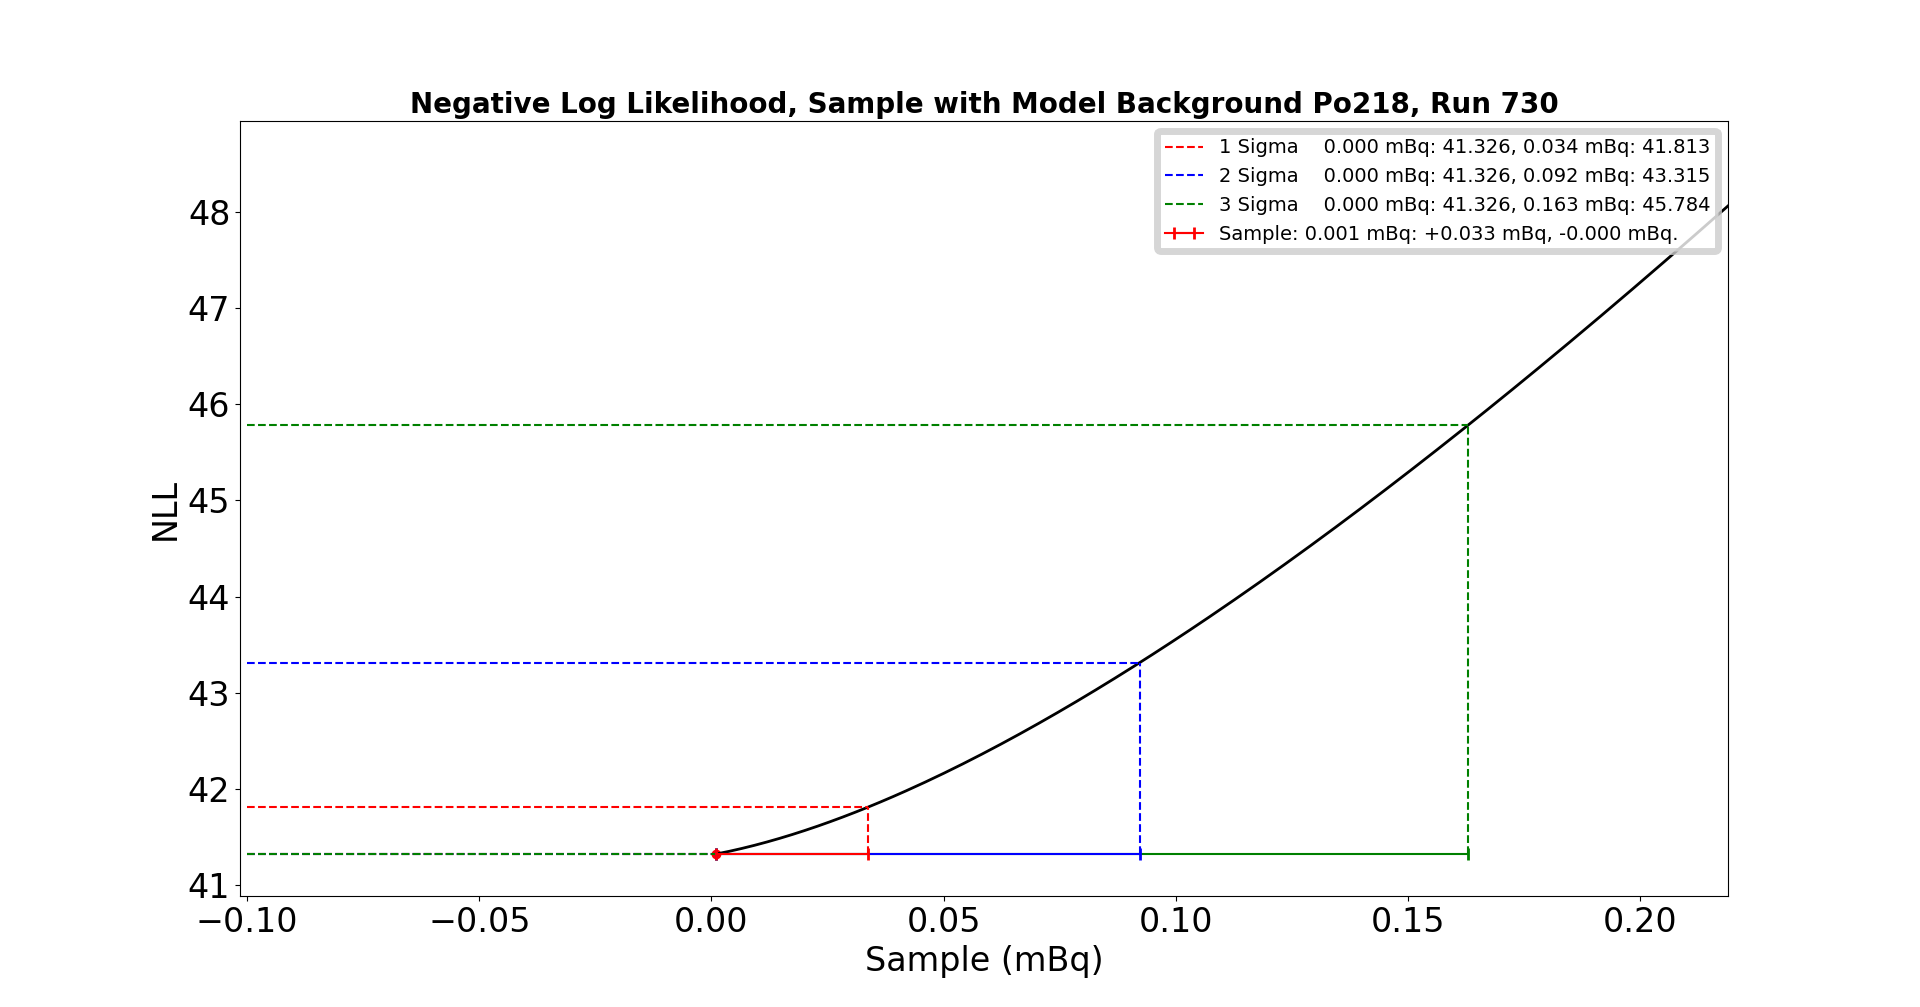
\includegraphics[width=0.9\textwidth]
            {assets/730/NLL218.png}
            \caption{This rate is used to determine the combined rate}
        \end{center}
    \end{figure}
\end{frame}

\begin{frame}{$^{214}$Po NLL, Run 730}
    \begin{figure}
        \begin{center}
            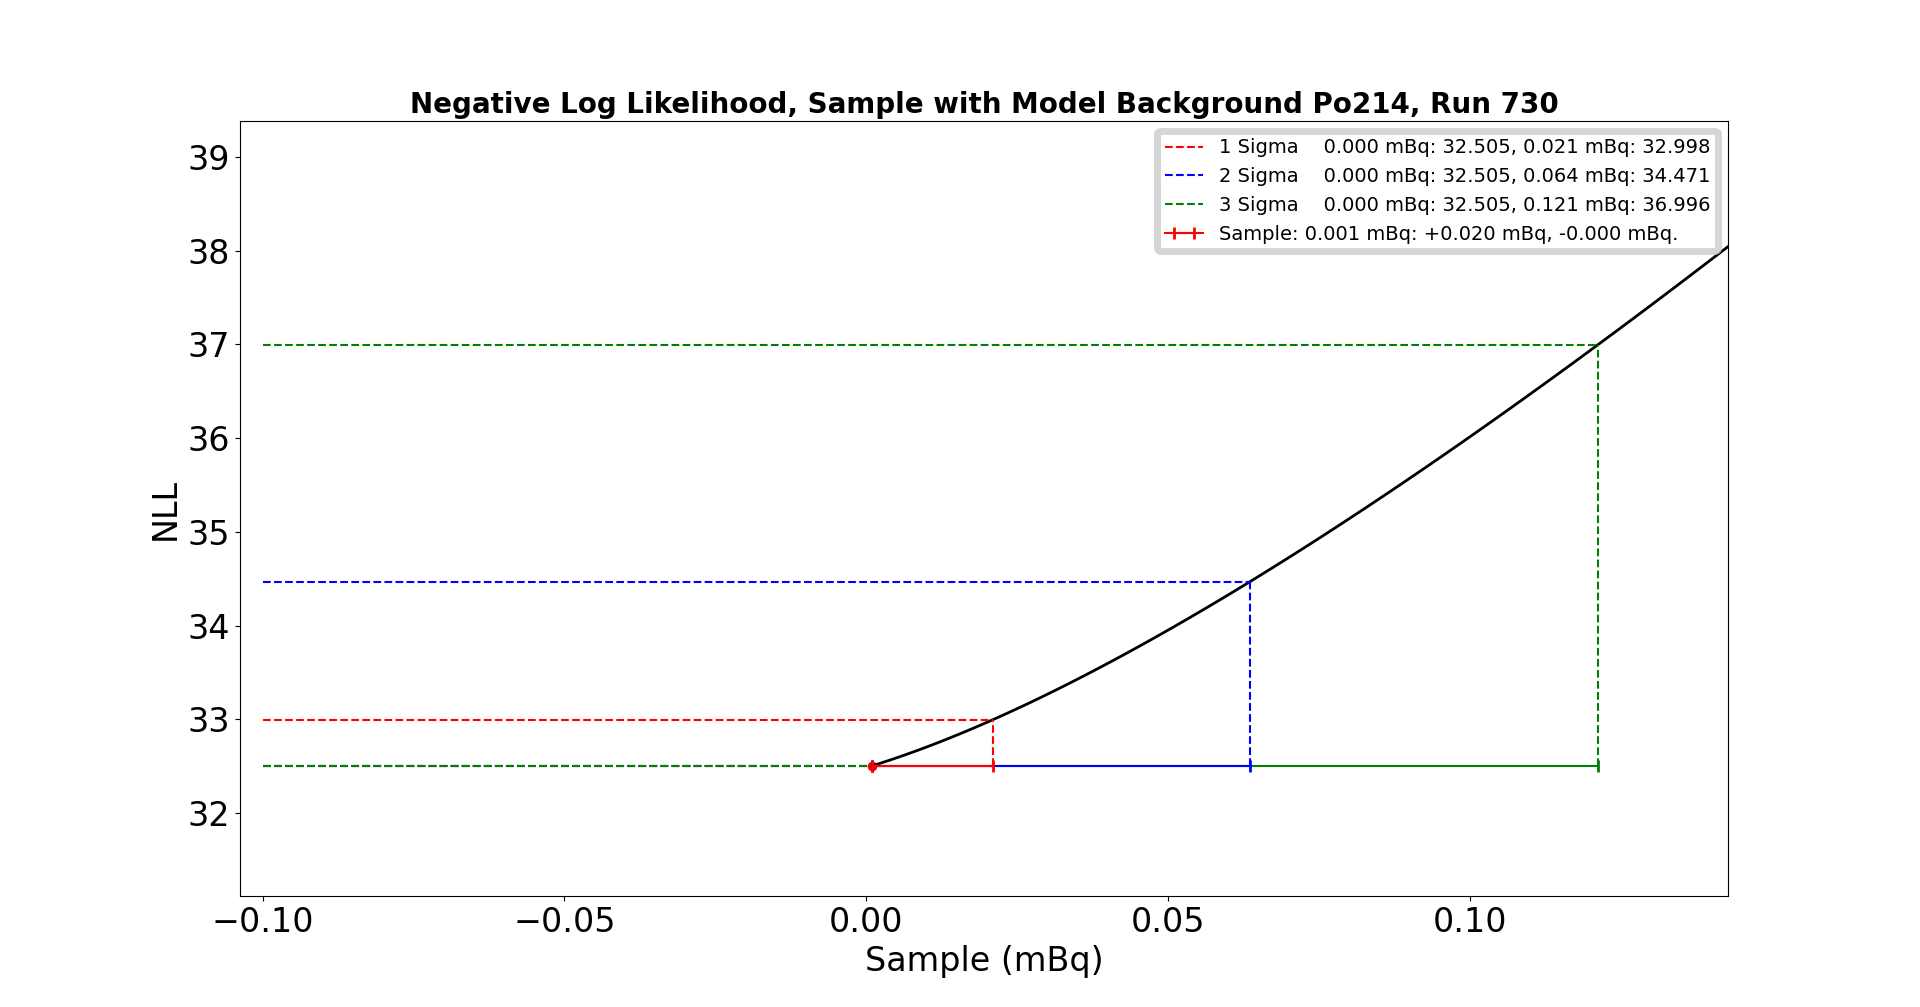
\includegraphics[width=0.9\textwidth]
            {assets/730/NLL214.png}
            \caption{This rate is used to determine the combined rate}
        \end{center}
    \end{figure}
\end{frame}

\begin{frame}{Live Time Efficiency}
    \begin{figure}
        \begin{center}
            \includegraphics[width=0.9\textwidth]
            {assets/730/LTE.png}
            \caption{Detector had relatively little dead time}
        \end{center}
    \end{figure}
\end{frame}

\begin{frame}{Notes on Run 730 Analysis}
    Run 730 exhibits such extreme shifts in gain that peak finding was impossible without removing 
    several hours of data.
    However, there is better resolution and the combined rate was able to be utilized for this run.


    \hyperlink{RvT_730}{\beamerbutton{Back to Rate vs Time Run 730}}
\end{frame}





\end{document}
